% !TEX program = xelatex
\documentclass[10pt,a4paper,oneside]{article}
\usepackage[utf8]{inputenc}
\usepackage{fontspec}
\usepackage{xeCJK}
\usepackage{geometry}
\usepackage{xcolor}
\usepackage{tikz}
\usepackage{graphicx}
\usepackage{tabularx}
\usepackage{booktabs}
\usepackage{array}
\usepackage{multicol}
\usepackage{enumitem}
\usepackage{microtype}
\usepackage{fancyhdr}
\usepackage{fontawesome5}
\usepackage{eso-pic}

\usetikzlibrary{shapes.geometric, arrows.meta, positioning, calc, backgrounds, shadows, fit}

% Set margins: 12mm left/right, 14mm top, 14mm bottom
\geometry{a4paper, top=14mm, bottom=14mm, left=12mm, right=12mm, headheight=0mm, headsep=0mm, footskip=0mm}

% CJK Font: Noto Sans CJK SC for Chinese Simplified
\setCJKmainfont{Noto Sans CJK SC}[
  BoldFont={Noto Sans CJK SC Bold},
]
\setCJKsansfont{Noto Sans CJK SC}[
  BoldFont={Noto Sans CJK SC Bold},
]
\setCJKmonofont{Noto Sans Mono CJK SC}

% Latin Font: DejaVu Sans for numbers, symbols, Latin text
\IfFontExistsTF{Segoe UI}{
  \setmainfont{Segoe UI}[
    BoldFont={Segoe UI Bold},
    ItalicFont={Segoe UI Italic},
    BoldItalicFont={Segoe UI Bold Italic}
  ]
}{
  \IfFontExistsTF{Arial}{
    \setmainfont{Arial}[
      BoldFont={Arial Bold},
      ItalicFont={Arial Italic},
      BoldItalicFont={Arial Bold Italic}
    ]
  }{
    \setmainfont{DejaVu Sans}[
      BoldFont={DejaVu Sans Bold},
      ItalicFont={DejaVu Sans Oblique},
      BoldItalicFont={DejaVu Sans Bold Oblique}
    ]
  }
}

% Color Palette - Luxury Corporate High-Tech
\definecolor{TTCDeepNavy}{RGB}{10, 25, 47}
\definecolor{TTCBlue}{RGB}{15, 60, 120}
\definecolor{TTCLightBlue}{RGB}{240, 246, 255}
\definecolor{TTCRed}{RGB}{214, 40, 40}
\definecolor{TTCCyan}{RGB}{0, 180, 216}
\definecolor{TTCGold}{RGB}{247, 127, 0}
\definecolor{TTCTextDark}{RGB}{30, 41, 59}
\definecolor{TTCTextMuted}{RGB}{100, 116, 139}
\definecolor{TTCBorder}{RGB}{203, 213, 225}

\newcolumntype{Y}{>{\centering\arraybackslash}X}
\newcolumntype{L}{>{\raggedright\arraybackslash}X}
\newcolumntype{R}{>{\raggedleft\arraybackslash}X}

\setlength{\parindent}{0pt}
\setlength{\parskip}{0pt}
\linespread{1.05}
\pagestyle{empty}

% Header & Footer Macros — Chinese Version
\newcommand{\pageheaderbar}[2]{%
  \begin{tikzpicture}[remember picture, overlay]
    \fill[TTCDeepNavy] (current page.north west) rectangle ([yshift=-10mm]current page.north east);
    \fill[TTCRed] ([yshift=-10mm]current page.north west) rectangle ([yshift=-11mm]current page.north east);
    \node[anchor=west, text=white, font=\fontsize{7.5}{9}\selectfont\bfseries] at ([xshift=12mm, yshift=-5mm]current page.north west) {
      \faBuilding\quad 新成功建筑科技股份公司 \textbullet\ TTC JSC
    };
    \node[anchor=east, text=TTCCyan, font=\fontsize{7.5}{9}\selectfont\bfseries] at ([xshift=-12mm, yshift=-5mm]current page.north east) {
      #1
    };
  \end{tikzpicture}%
}

\newcommand{\pagefooterbar}[1]{%
  \begin{tikzpicture}[remember picture, overlay]
    \fill[TTCDeepNavy] (current page.south west) rectangle ([yshift=8mm]current page.south east);
    \fill[TTCCyan] ([yshift=8mm]current page.south west) rectangle ([yshift=8.8mm]current page.south east);
    \node[anchor=west, text=white, font=\fontsize{6.8}{8}\selectfont] at ([xshift=12mm, yshift=4mm]current page.south west) {
      \faPhone*\ +84 976 447 766 \quad\textbullet\quad \faEnvelope\ info@tanthanhcongjsc.com \quad\textbullet\quad \faGlobe\ https://tanthanhcongjsc.com
    };
    \node[anchor=east, text=white, font=\fontsize{7}{8}\selectfont\bfseries] at ([xshift=-12mm, yshift=4mm]current page.south east) {
      #1
    };
  \end{tikzpicture}%
}

% Header/footer anchored directly to shipout; use for dense TikZ case-study pages.
\newcommand{\casepagebars}[2]{%
  \AddToShipoutPictureFG*{%
    \AtPageUpperLeft{%
      \begin{tikzpicture}[x=1mm,y=1mm]
        \path[use as bounding box] (0,0) rectangle (0,0);
        \fill[TTCDeepNavy] (0,0) rectangle (210,-10);
        \fill[TTCRed] (0,-10) rectangle (210,-11);
        \node[anchor=west,text=white,font=\fontsize{7.5}{9}\selectfont\bfseries] at (12,-5)
          {\faBuilding\quad 新成功建筑科技股份公司 \textbullet\ TTC JSC};
        \node[anchor=east,text=TTCCyan,font=\fontsize{7.5}{9}\selectfont\bfseries] at (198,-5)
          {#1};
      \end{tikzpicture}%
    }%
    \AtPageLowerLeft{%
      \begin{tikzpicture}[x=1mm,y=1mm]
        \path[use as bounding box] (0,0) rectangle (0,0);
        \begin{scope}[opacity=.075]
          \draw[TTCBlue,line width=.55pt]
            (12,9) -- (12,15) -- (28,15) -- (35,22) -- (51,22) -- (58,15)
            -- (78,15) -- (84,28) -- (90,28) -- (90,15) -- (110,15)
            -- (119,23) -- (137,23) -- (146,15) -- (162,15)
            -- (169,20) -- (191,20) -- (198,14) -- (198,9);
          \draw[TTCBlue,line width=.35pt] (12,9) -- (198,9);
          \draw[TTCBlue,line width=.35pt] (35,22) -- (43,15) -- (51,22);
          \draw[TTCBlue,line width=.35pt] (119,23) -- (128,15) -- (137,23);
          \draw[TTCBlue,line width=.35pt] (84,15) -- (90,28);
          \draw[TTCBlue,line width=.35pt] (96,15) -- (96,31) -- (101,31) -- (101,15);
          \foreach \x in {18,24,64,70,116,152,158,176,184,192}{
            \draw[TTCBlue,line width=.25pt] (\x,10.5) -- (\x,14);
          }
        \end{scope}
        \fill[TTCDeepNavy] (0,0) rectangle (210,8);
        \fill[TTCCyan] (0,8) rectangle (210,8.8);
        \node[anchor=west,text=white,font=\fontsize{6.8}{8}\selectfont] at (12,4)
          {\faPhone*\ +84 976 447 766 \quad\textbullet\quad \faEnvelope\ info@tanthanhcongjsc.com \quad\textbullet\quad \faGlobe\ https://tanthanhcongjsc.com};
        \node[anchor=east,text=white,font=\fontsize{7}{8}\selectfont\bfseries] at (198,4)
          {#2};
      \end{tikzpicture}%
    }%
  }%
}

% Section Header Brand Macro
\newcommand{\secbrand}[2]{%
  \noindent\begin{tikzpicture}
    \fill[TTCRed] (0,0) rectangle (4mm,10mm);
    \node[anchor=west, align=left, inner sep=0pt] at (6mm, 5mm) {
      {\fontsize{13}{15}\selectfont\bfseries\color{TTCBlue} #1}\\[1.5pt]
      {\fontsize{7.2}{8.8}\selectfont\itshape\color{TTCTextMuted} #2}
    };
  \end{tikzpicture}\par\vspace{1.5mm}%
}

\begin{document}
% ============================================================
% TRANG 01: TRANG BÌA CHÍNH — COMPANY PROFILE 2026
% ============================================================
\thispagestyle{empty}
\begin{tikzpicture}[remember picture, overlay]
  % 1. Hero image
  \node[anchor=center, inner sep=0pt] at (current page.center) {
    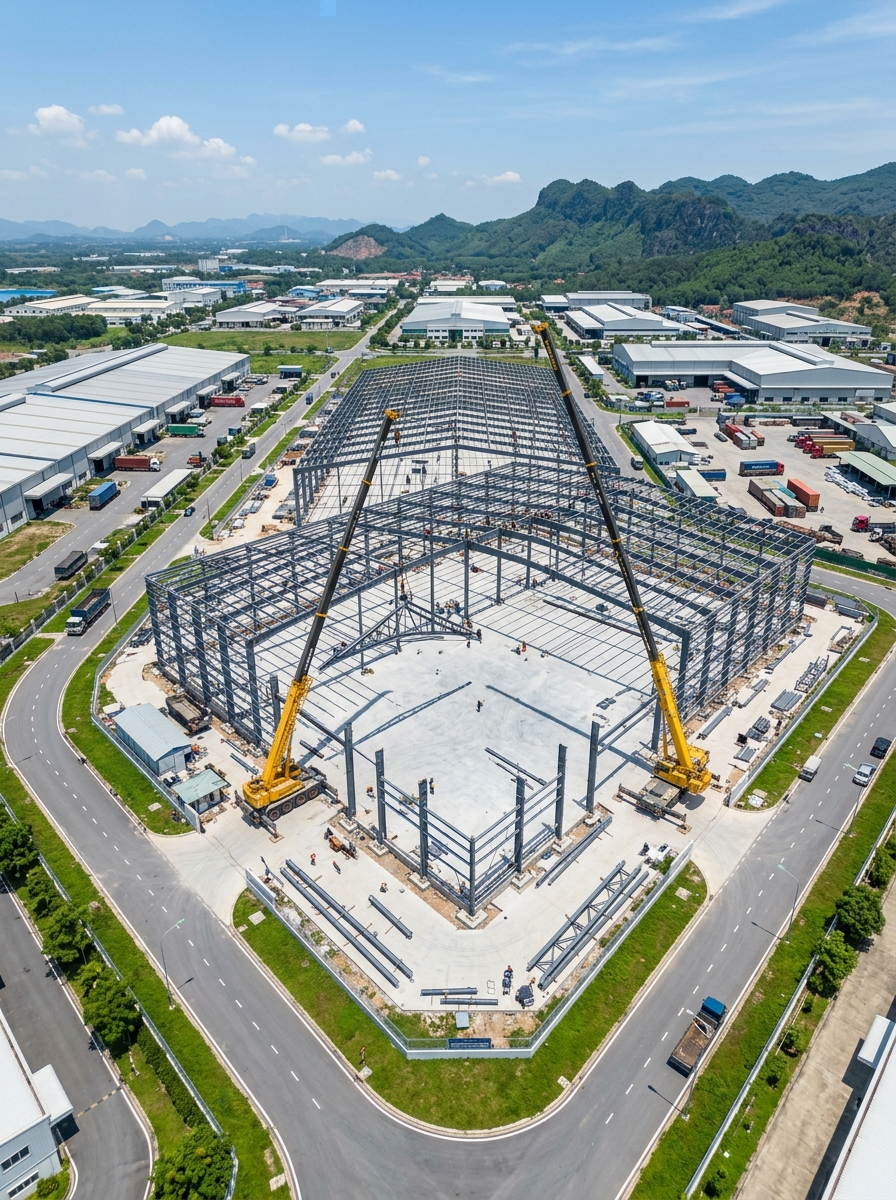
\includegraphics[height=\paperheight]{../../public/executive-cover-hero.jpg}
  };

  % 2. Gradient overlay
  \shade[
    left color=TTCDeepNavy!96!black,
    right color=transparent,
    opacity=0.70
  ] (current page.south west) rectangle (current page.north east);

  % 3. TTC recognition bar and logo lock-up
  \fill[TTCRed] (current page.north west) rectangle ++(\paperwidth, -2.2mm);
  \node[anchor=north west, fill=white, fill opacity=0.96, text opacity=1,
        rounded corners=1.5pt, inner xsep=5mm, inner ysep=3.8mm]
    at ([xshift=15mm,yshift=-13mm]current page.north west) {
      
\includegraphics[width=48mm]{../../public/logo-ttc-removebg-DNXrVdJp.png}
    };
  \node[anchor=north east, text=white, inner sep=0pt] at ([xshift=-15mm,yshift=-15mm]current page.north east) {
    {\fontsize{8}{10}\selectfont\bfseries COMPANY PROFILE \;|\; 2026}
  };

  % 4. Title block
  \node[anchor=west, align=left, text width=135mm, inner sep=0pt]
    at ([xshift=16mm,yshift=160mm]current page.south west) {
      {\fontsize{7.8}{9.6}\selectfont\bfseries\color{TTCRed} TAN THANH CONG TECHNOLOGY CONSTRUCTION JOINT STOCK COMPANY}\\[6mm]
      {\fontsize{42}{50}\selectfont\bfseries\color{white} 企业能力简介}\\[5mm]
      {\color{TTCRed}\rule{73mm}{2.8pt}}\\[5mm]
      {\fontsize{17}{20}\selectfont\bfseries\color{white} COMPANY PROFILE}\\[8mm]
      {\fontsize{15}{18}\selectfont\bfseries\color{white} 新一代工业 EPC 总承包商}\\[3mm]
      {\fontsize{9.5}{12}\selectfont\color{white!88!gray} Turnkey Industrial EPC General Contractor}
    };

  % 5. Proof points
  \node[anchor=south west, align=left, fill=TTCDeepNavy!92!black, fill opacity=0.84,
        text=white, text opacity=1, rounded corners=1.5pt, inner xsep=6mm, inner ysep=4mm]
    at ([xshift=15mm,yshift=31mm]current page.south west) {
      {\fontsize{12}{14}\selectfont\bfseries 150+ 工业项目 \qquad 建设部二级资质 \qquad ISO 9001 / 14001 / 45001}\\[1.2mm]
      {\fontsize{7}{8.5}\selectfont\color{white!82!gray}经现场验证的工业总承包综合实力}
    };

  % 6. Legal identity
  \node[anchor=south west, text=white, inner sep=0pt] at ([xshift=15mm,yshift=19mm]current page.south west) {
    {\fontsize{6.6}{8.2}\selectfont\bfseries 新成功建筑科技股份公司 \textbullet\ TAN THANH CONG TECH JSC}
  };

  % 7. Persistent contact footer
  \fill[TTCDeepNavy!97!black] (current page.south west) rectangle ++(\paperwidth, 11mm);
  \fill[TTCRed] ([yshift=11mm]current page.south west) rectangle ++(\paperwidth, 1.2mm);
  \node[anchor=south, text=white, inner sep=0pt] at ([yshift=3.4mm]current page.south) {
    {\fontsize{6.8}{8.2}\selectfont
      \faPhone\ +84 976 447 766 \quad\textbullet\quad
      \faEnvelope\ info@tanthanhcongjsc.com \quad\textbullet\quad
      \faGlobe\ tanthanhcongjsc.com \quad\textbullet\quad
      \faAward\ 越南建设部二级施工资质}
  };
\end{tikzpicture}
\mbox{}
\newpage

% ============================================================
% TRANG 02: MỤC LỤC ĐIỀU HƯỚNG & THÔNG TIN PHÁP NHÂN TÓM TẮT
% ============================================================
\pageheaderbar{总目录概览与法人信息}{第02页}
\pagefooterbar{第02页}

\begin{tikzpicture}[remember picture, overlay]
  \node[opacity=0.025, scale=4.2, font=\bfseries\sffamily, text=TTCBlue]
    at ([xshift=30mm,yshift=-8mm]current page.center) {TTC};
  \fill[TTCRed, opacity=0.05] ([xshift=12mm,yshift=18mm]current page.south west)
    rectangle ([xshift=18mm,yshift=248mm]current page.south west);
\end{tikzpicture}

\begin{minipage}[t][246mm]{\textwidth}
\secbrand{总目录概览}{Executive Contents — 06 Core Sections}

{\fontsize{9.2}{11.5}\selectfont\color{TTCTextMuted}
本报告按06大核心板块编排，便于业主快速查阅；各专题详见对应页面。}\\[3mm]

\newcommand{\toccard}[5]{%
  \begin{tikzpicture}
    \node[rounded corners=3pt, fill=white, draw=TTCBorder, line width=0.8pt,
          minimum width=90mm, minimum height=52mm, text width=79mm, inner sep=5.5mm, align=left] {
      {\fontsize{18}{19}\selectfont\bfseries\color{TTCRed} #1}\hspace{3mm}
      {\fontsize{8.2}{9.5}\selectfont\bfseries\color{TTCRed} 第 #2 页}\\[1.5mm]
      {\fontsize{11.2}{13.2}\selectfont\bfseries\color{TTCBlue} #3}\\[0.3mm]
      {\fontsize{7.2}{8.8}\selectfont\itshape\color{TTCTextMuted} #4}\\[3mm]
      {\fontsize{8.2}{10.5}\selectfont\color{TTCTextDark} #5}
    };
  \end{tikzpicture}%
}

\noindent
\begin{tabular}{@{}p{91mm}@{\hspace{4mm}}p{91mm}@{}}
\toccard{I}{01--07}{公司概况与核心能力}{Company profile \& credentials}{总经理致辞 \textbullet\ 愿景与价值观 \textbullet\ 产业生态 \textbullet\ 法人与管理团队} &
\toccard{IV}{14--19}{EPC解决方案与建筑科技}{EPC, ConTech \& ESG}{Fast-track快速推进 \textbullet\ BIM 5D/AI \textbullet\ ESG低碳 \textbullet\ QA/QC与HSE} \\[3.5mm]
\toccard{II}{08--10}{财务实力与精英团队}{Financial capacity \& people}{独立预算管控 \textbullet\ 2500亿授信担保 \textbullet\ 2850+人才 \textbullet\ 安全文化} &
\toccard{V}{20--30}{重点项目与国际客户}{Projects \& valued partners}{150+工业项目 \textbullet\ 06大经典案例 \textbullet\ 严控供应链 \textbullet\ FDI伙伴} \\[3.5mm]
\toccard{III}{11--13}{生产制造与FIDIC管理}{PEB \& project control}{3万吨PEB制造网络 \textbullet\ 3000亿重型机械 \textbullet\ FIDIC八阶段流程} &
\toccard{VI}{31--36}{金牌承诺与长期合作}{Commitments \& support}{资质荣誉 \textbullet\ 20+省市施工覆盖 \textbullet\ 战略愿景 \textbullet\ 24个月保修与联系}
\end{tabular}

\vspace{4.5mm}

\noindent
\begin{tikzpicture}
  \node[rounded corners=3pt, fill=TTCLightBlue, draw=TTCBorder, line width=0.8pt,
        minimum width=186mm, text width=172mm, inner sep=7.5mm] {
    {\fontsize{10.5}{12.5}\selectfont\bfseries\color{TTCBlue} \faIdCard\quad 企业法人信息摘要}
    \hfill {\fontsize{7.2}{8.8}\selectfont\color{TTCRed}\bfseries 详细资质认证：第 06 页}\\[1.5mm]
    {\fontsize{6.2}{7.5}\selectfont\color{TTCTextMuted}\bfseries
    TAN THANH CONG TECHNOLOGY CONSTRUCTION JOINT STOCK COMPANY}\\[3mm]
    \renewcommand{\arraystretch}{1.28}
    {\fontsize{8.2}{10.2}\selectfont
    \begin{tabularx}{\linewidth}{@{}p{30mm}X@{\hspace{5mm}}p{28mm}X@{}}
      \textbf{企业名称} & \textbf{新成功建筑科技股份公司} (TTC JSC) &
      \textbf{税务登记号} & \textbf{0107090447} \\
      \textbf{法定代表人} & \textbf{范辉新 (PHẠM HUY TÂN)} — 总经理 &
      \textbf{资质等级} & 越南建设部二级资质 \textbullet\ ISO 9001/14001/45001 \\
      \textbf{注册地址} & Số 39, ngõ 292 Kim Giang, Đại Kim, Hà Nội &
      \textbf{办公地址} & Số 19N7B, KĐT Trung Hòa Nhân Chính, Hà Nội \\
      \textbf{联系电话} & +84 976 447 766 \textbullet\ info@tanthanhcongjsc.com &
      \textbf{官方网站} & tanthanhcongjsc.com
    \end{tabularx}}
  };
\end{tikzpicture}
\end{minipage}
\newpage

% ============================================================
% TRANG 03: THÔNG ĐIỆP TỪ TỔNG GIÁM ĐỐC — LEADERSHIP MESSAGE
% ============================================================
\pageheaderbar{总经理致辞}{第03页}
\pagefooterbar{第03页}

\begin{tikzpicture}[remember picture, overlay]
  \node[opacity=0.025, scale=4.0, font=\bfseries\sffamily, text=TTCBlue]
    at ([xshift=-25mm,yshift=-25mm]current page.center) {LEADERSHIP};
  \fill[TTCRed, opacity=0.045] ([xshift=12mm,yshift=18mm]current page.south west)
    rectangle ([xshift=18mm,yshift=248mm]current page.south west);
\end{tikzpicture}

\begin{minipage}[t][246mm]{\textwidth}
\secbrand{总经理致辞}{Leadership Message — Building Trust Through Every Commitment}

\vspace{2mm}

\noindent
\begin{tabular}{@{}p{106mm}@{\hspace{4mm}}p{76mm}@{}}
  \begin{tikzpicture}
    \path[use as bounding box] (0,0) rectangle (106mm,170mm);
    \draw[TTCRed, line width=2.2pt] (0,169mm) -- (26mm,169mm);
    \node[anchor=north west, align=left, text width=98mm, inner sep=0pt] at (0,165mm) {
      {\fontsize{8.5}{10}\selectfont\bfseries\color{TTCRed} TTC 的核心经营理念}\\[4mm]
      {\fontsize{18}{22}\selectfont\bfseries\color{TTCBlue}
      “质量即荣誉。\\
      安全即生命。\\
      进度即承诺。”}\\[6mm]
      {\fontsize{10}{12}\selectfont\bfseries\color{TTCBlue}
      尊敬的投资方、客户及合作伙伴：}\\[3mm]
      {\fontsize{9}{13}\selectfont\color{TTCTextDark}
      我谨代表\textbf{新成功建筑科技股份公司}（TTC JSC）全体管理团队及员工，衷心感谢各位在TTC发展历程中所给予的坚定信任与支持。\\[3mm]

      十余年深耕工业建筑领域，让我们深刻理解：一个卓越的工程必须同时满足\textbf{质量、安全、进度与投资效益}。因此，TTC始终践行\textbf{EPC一站式总承包模式}，深度融合价值工程（Value Engineering）、BIM 5D协同与国际标准现场管理体系。\\[3mm]

      依托年产能30,000吨的PEB战略制造网络与实战型工程师团队，我们承诺为每座工厂量身定制最优技术方案，从方案设计、施工装配到竣工交付与全寿命运维实行全程透明管控。\\[3mm]

      TTC不仅是总承包商，更是与业主\textbf{共创长期价值的战略合作伙伴}。}\\[5mm]
      {\fontsize{9}{11}\selectfont\itshape\color{TTCTextMuted} 此致敬礼，}
    };
  \end{tikzpicture}
  &
  \begin{tikzpicture}
    \path[use as bounding box] (0,0) rectangle (76mm,170mm);
    \fill[TTCLightBlue] (0,0) rectangle (76mm,170mm);
    \draw[TTCBorder, line width=0.8pt] (0,0) rectangle (76mm,170mm);
    \fill[TTCRed] (0,0) rectangle (3mm,170mm);

    \node[anchor=north, inner sep=0pt] at (39.5mm,168mm) {
      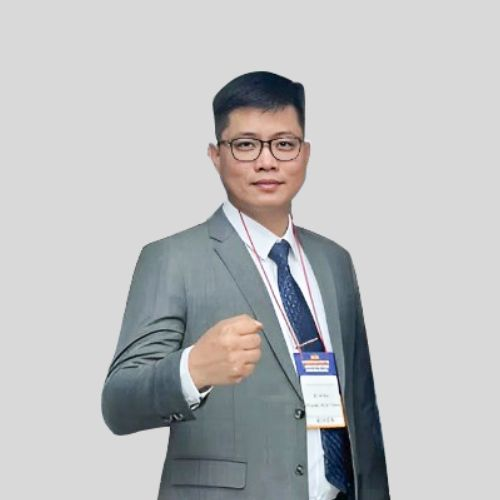
\includegraphics[trim=90 0 90 0,clip,height=116mm]{../tan_avatar.jpg}
    };

    \fill[TTCDeepNavy!97!black] (3mm,0) rectangle (76mm,54mm);
    \fill[TTCRed] (3mm,54mm) rectangle (76mm,56mm);
    \node[anchor=north west, align=left, text width=62mm, inner sep=0pt]
      at (10mm,46mm) {
        {\fontsize{7}{8.5}\selectfont\bfseries\color{TTCRed} 总经理 / CEO}\\[2mm]
        {\fontsize{14}{17}\selectfont\bfseries\color{white} 范辉新}\\[2mm]
        {\fontsize{7.5}{9.5}\selectfont\color{white!78!gray}
        新成功建筑科技股份公司}\\[4mm]
        {\fontsize{7.2}{9}\selectfont\bfseries\color{white!68!gray} TÂN THÀNH CÔNG \textbullet\ TTC JSC}
      };
  \end{tikzpicture}
\end{tabular}

\vspace{5mm}

\noindent
\begin{tabular}{@{}p{58mm}@{\hspace{6mm}}p{58mm}@{\hspace{6mm}}p{58mm}@{}}
  \begin{tikzpicture}
    \node[rounded corners=3pt, fill=TTCDeepNavy!97!black, minimum width=58mm,
          minimum height=43mm, text width=48mm, align=center, inner sep=5mm] {
      {\fontsize{17}{19}\selectfont\bfseries\color{white} 01}\\[1mm]
      {\fontsize{9}{11}\selectfont\bfseries\color{TTCRed} EPC一站式总包}\\[2mm]
      {\fontsize{7.3}{9}\selectfont\color{white!78!gray}Design \textbullet\ Build \textbullet\ Turnkey}
    };
  \end{tikzpicture}
  &
  \begin{tikzpicture}
    \node[rounded corners=3pt, fill=TTCLightBlue, draw=TTCBorder, line width=0.8pt,
          minimum width=58mm, minimum height=43mm, text width=48mm, align=center, inner sep=5mm] {
      {\fontsize{17}{19}\selectfont\bfseries\color{TTCRed} 10--15\%}\\[1mm]
      {\fontsize{9}{11}\selectfont\bfseries\color{TTCBlue} 优化投资成本}\\[2mm]
      {\fontsize{7.3}{9}\selectfont\color{TTCTextMuted}Value Engineering}
    };
  \end{tikzpicture}
  &
  \begin{tikzpicture}
    \node[rounded corners=3pt, fill=TTCLightBlue, draw=TTCBorder, line width=0.8pt,
          minimum width=58mm, minimum height=43mm, text width=48mm, align=center, inner sep=5mm] {
      {\fontsize{15}{18}\selectfont\bfseries\color{TTCRed} ZERO}\\[1mm]
      {\fontsize{9}{11}\selectfont\bfseries\color{TTCBlue} 零事故安全}\\[2mm]
      {\fontsize{7.3}{9}\selectfont\color{TTCTextMuted}HSE Commitment}
    };
  \end{tikzpicture}
\end{tabular}

\vspace{6mm}

\noindent
\begin{tikzpicture}
  \node[rounded corners=2pt, fill=white, draw=TTCRed, line width=0.9pt,
        minimum width=186mm, minimum height=15mm, align=center, inner sep=3mm] {
    {\fontsize{10}{12}\selectfont\bfseries\color{TTCBlue}
    共创长期价值 \quad\textbullet\quad BUILDING ENDURING VALUE}
  };
\end{tikzpicture}
\end{minipage}
\newpage

% ============================================================
% TRANG 04: KẾT CẤU VƯƠN CAO — HÀNH TRÌNH & GIÁ TRỊ CỐT LÕI
% ============================================================
\pageheaderbar{发展历程与核心价值观}{第04页}
\pagefooterbar{第04页}

\begin{tikzpicture}[remember picture, overlay]
  \node[opacity=0.022, scale=4.0, font=\bfseries\sffamily, text=TTCBlue]
    at ([xshift=15mm,yshift=-18mm]current page.center) {BUILDING THE FUTURE};
\end{tikzpicture}

\begin{minipage}[t][246mm]{\textwidth}
\secbrand{发展历程与核心价值观}{From Mechanical Foundations to a Next-Generation EPC General Contractor}

\vspace{1mm}

\noindent
\begin{tikzpicture}
  \node[anchor=west, align=left, inner sep=0pt] at (0,7mm) {
    {\fontsize{16}{19}\selectfont\bfseries\color{TTCBlue}
    从精密机械基础到新一代工业EPC总承包商}\\[1.5mm]
    {\fontsize{7.8}{9.5}\selectfont\color{TTCTextMuted}
    以坚实执行力、数字化技术与永恒核心价值观铸就的发展之路。}
  };
  \fill[TTCRed] (0,0) rectangle (52mm,1.4mm);
\end{tikzpicture}

\vspace{3mm}

\noindent
\begin{tikzpicture}[x=1mm,y=1mm]
  \path[use as bounding box] (0,0) rectangle (186,112);
  \fill[TTCLightBlue!55!white] (0,0) rectangle (186,112);
  \draw[TTCBorder, line width=0.8pt, rounded corners=3pt] (0,0) rectangle (186,112);
  \draw[TTCBlue!7!white, line width=0.35pt] (0,0) grid[step=10mm] (186,112);

  % Stepped structural spine
  \draw[TTCBlue!10!white, line width=7pt, line join=round]
    (16,19) -- (44,19) -- (52,40) -- (76,40) -- (84,61) --
    (116,61) -- (124,82) -- (155,82) -- (163,105) -- (180,105);
  \draw[TTCBlue!28!white, line width=1pt, line join=round]
    (12,14) -- (41,14) -- (49,35) -- (73,35) -- (81,56) --
    (113,56) -- (121,77) -- (152,77) -- (160,100) -- (177,100);
  \draw[TTCRed, line width=3.2pt, line join=round]
    (16,19) -- (44,19) -- (52,40) -- (76,40) -- (84,61) --
    (116,61) -- (124,82) -- (155,82) -- (163,105) -- (180,105);
  \draw[TTCRed, line width=1.1pt, -{Stealth[length=4mm]}] (180,105) -- (184,109);

  % 2015
  \fill[white] (16,19) circle (3.4);
  \draw[TTCRed, line width=1.5pt] (16,19) circle (3.4);
  \fill[TTCRed] (16,19) circle (1.35);
  \node[anchor=south west, align=left, text width=38mm, fill=TTCLightBlue!86!white,
        fill opacity=0.94, text opacity=1, rounded corners=1.5pt, inner sep=1mm] at (7,25) {
    {\fontsize{18}{20}\selectfont\bfseries\color{TTCRed} 2015}\\[-0.5mm]
    {\fontsize{8.5}{10}\selectfont\bfseries\color{TTCBlue} 创立起步}\\[1mm]
    {\fontsize{7.2}{9}\selectfont\color{TTCTextDark}精密机械加工与钢结构\\工程安装技术积累。}
  };

  % 2018
  \fill[white] (55,40) circle (3.4);
  \draw[TTCRed, line width=1.5pt] (55,40) circle (3.4);
  \fill[TTCRed] (55,40) circle (1.35);
  \node[anchor=north west, align=left, text width=38mm, fill=TTCLightBlue!86!white,
        fill opacity=0.94, text opacity=1, rounded corners=1.5pt, inner sep=1mm] at (38,29) {
    {\fontsize{18}{20}\selectfont\bfseries\color{TTCRed} 2018}\\[-0.5mm]
    {\fontsize{8.5}{10}\selectfont\bfseries\color{TTCBlue} 扩张跨越}\\[1mm]
    {\fontsize{7.2}{9}\selectfont\color{TTCTextDark}PEB联合制造网络与\\工业园区基建总承包。}
  };

  % 2022
  \fill[white] (94,61) circle (3.4);
  \draw[TTCRed, line width=1.5pt] (94,61) circle (3.4);
  \fill[TTCRed] (94,61) circle (1.35);
  \node[anchor=south west, align=left, text width=39mm, fill=TTCLightBlue!86!white,
        fill opacity=0.94, text opacity=1, rounded corners=1.5pt, inner sep=1mm] at (71,67) {
    {\fontsize{18}{20}\selectfont\bfseries\color{TTCRed} 2022}\\[-0.5mm]
    {\fontsize{8.5}{10}\selectfont\bfseries\color{TTCBlue} 资质突破}\\[1mm]
    {\fontsize{7.2}{9}\selectfont\color{TTCTextDark}获建设部二级总包资质，\\承建多座大型FDI厂房。}
  };

  % 2026
  \fill[white] (134,82) circle (3.4);
  \draw[TTCRed, line width=1.5pt] (134,82) circle (3.4);
  \fill[TTCRed] (134,82) circle (1.35);
  \node[anchor=north west, align=left, text width=42mm, fill=TTCLightBlue!86!white,
        fill opacity=0.94, text opacity=1, rounded corners=1.5pt, inner sep=1mm] at (119,68) {
    {\fontsize{18}{20}\selectfont\bfseries\color{TTCRed} 2026}\\[-0.5mm]
    {\fontsize{8.5}{10}\selectfont\bfseries\color{TTCBlue} 科技转型}\\[1mm]
    {\fontsize{7.2}{9}\selectfont\color{TTCTextDark}150+工业项目 \textbullet\ 20+省市\\PEB年产能达30,000吨。}
  };

  % 2030
  \fill[white] (176,105) circle (3.4);
  \draw[TTCRed, line width=1.5pt] (176,105) circle (3.4);
  \fill[TTCRed] (176,105) circle (1.35);
  \node[anchor=north east, align=right, text width=40mm, fill=TTCLightBlue!86!white,
        fill opacity=0.94, text opacity=1, rounded corners=1.5pt, inner sep=1mm] at (178,98) {
    {\fontsize{18}{20}\selectfont\bfseries\color{TTCRed} 2030}\\[-0.5mm]
    {\fontsize{8.5}{10}\selectfont\bfseries\color{TTCBlue} 国际愿景}\\[1mm]
    {\fontsize{7.2}{9}\selectfont\color{TTCTextDark}ConTech建筑科技 \textbullet\ ESG\\进军东南亚国际市场。}
  };
\end{tikzpicture}

\vspace{4mm}

\noindent
\begin{tikzpicture}[x=1mm,y=1mm]
  \path[use as bounding box] (0,0) rectangle (186,112);
  \clip[rounded corners=3pt] (0,0) rectangle (186,112);
  \node[anchor=center, inner sep=0pt] at (93,56) {
    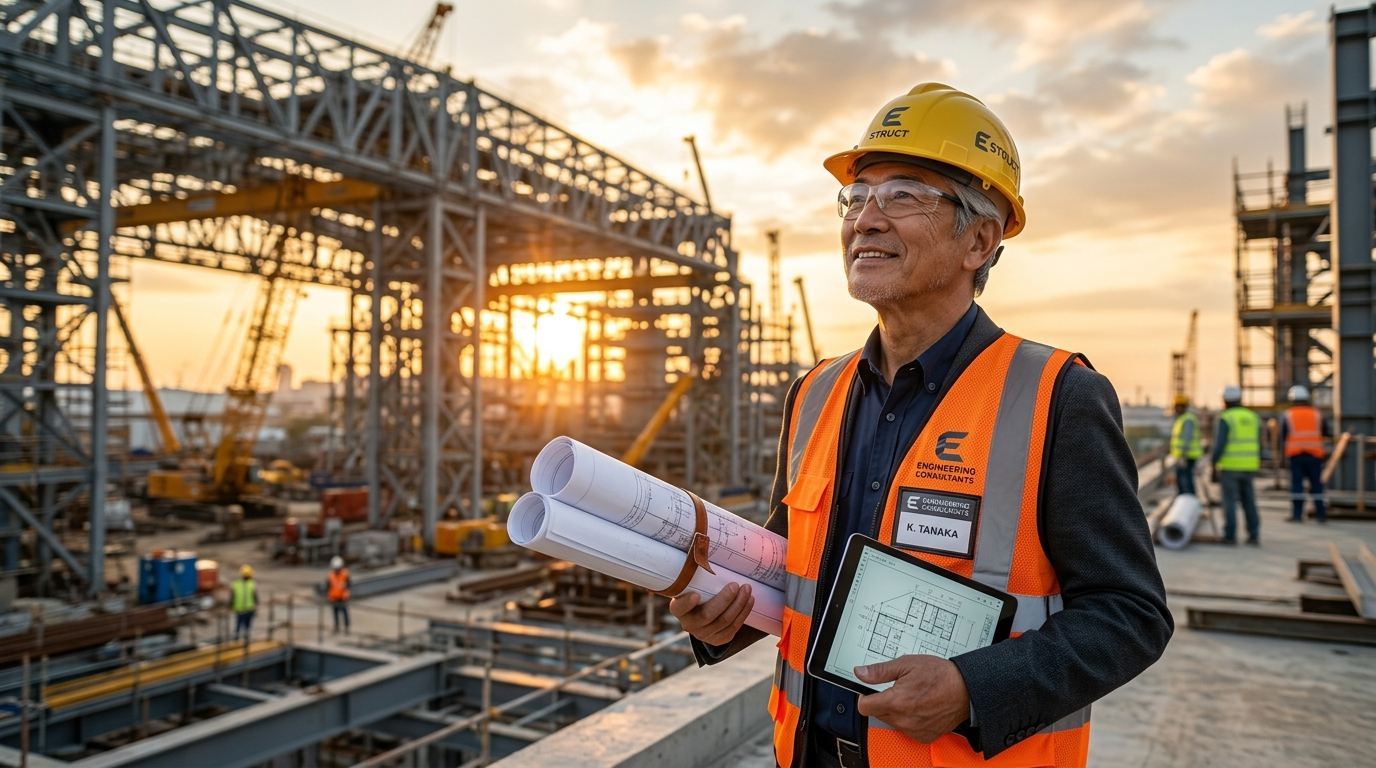
\includegraphics[height=112mm]{assets/milestones_engineer_hero.jpg}
  };
  \shade[left color=TTCDeepNavy!98!black, right color=transparent, opacity=0.82]
    (0,31) rectangle (142,112);
  \node[anchor=north west, align=left, text width=112mm, inner sep=0pt] at (8,104) {
    {\fontsize{12}{14}\selectfont\bfseries\color{white}五大核心价值观 — 铸就每一项工程的基石}\\[1.5mm]
    {\fontsize{7.5}{9}\selectfont\color{white!82!gray}The core values that sustain every commitment and project.}
  };

  \fill[TTCDeepNavy!97!black, opacity=0.96] (0,0) rectangle (37.2,31);
  \fill[TTCDeepNavy!91!black, opacity=0.96] (37.2,0) rectangle (74.4,31);
  \fill[TTCDeepNavy!97!black, opacity=0.96] (74.4,0) rectangle (111.6,31);
  \fill[TTCDeepNavy!91!black, opacity=0.96] (111.6,0) rectangle (148.8,31);
  \fill[TTCDeepNavy!97!black, opacity=0.96] (148.8,0) rectangle (186,31);
  \fill[TTCRed] (0,31) rectangle (186,32.3);

  \node[align=center, text=white] at (18.6,15.5) {
    {\fontsize{14}{16}\selectfont\bfseries 信}\\[1mm]
    {\fontsize{6.8}{8}\selectfont\color{white!72!gray}TRUST \& INTEGRITY}
  };
  \node[align=center, text=white] at (55.8,15.5) {
    {\fontsize{14}{16}\selectfont\bfseries 心}\\[1mm]
    {\fontsize{6.8}{8}\selectfont\color{white!72!gray}DEDICATION}
  };
  \node[align=center, text=white] at (93,15.5) {
    {\fontsize{14}{16}\selectfont\bfseries 智}\\[1mm]
    {\fontsize{6.8}{8}\selectfont\color{white!72!gray}INNOVATION}
  };
  \node[align=center, text=white] at (130.2,15.5) {
    {\fontsize{14}{16}\selectfont\bfseries 速}\\[1mm]
    {\fontsize{6.8}{8}\selectfont\color{white!72!gray}FAST-TRACK}
  };
  \node[align=center, text=white] at (167.4,15.5) {
    {\fontsize{14}{16}\selectfont\bfseries 安}\\[1mm]
    {\fontsize{6.8}{8}\selectfont\color{white!72!gray}HSE \& SAFETY}
  };
\end{tikzpicture}
\end{minipage}
\newpage

% ============================================================
% TRANG 05: INTEGRATED FACTORY BLUEPRINT
% ============================================================
\pageheaderbar{EPC总承包生态系统与研发技术}{第05页}
\pagefooterbar{第05页}

\begin{tikzpicture}[remember picture, overlay]
  \draw[TTCBlue!6!white, line width=0.45pt]
    ([xshift=15mm,yshift=18mm]current page.south west)
    grid[step=8mm]
    ([xshift=195mm,yshift=42mm]current page.south west);
\end{tikzpicture}

\begin{minipage}[t][246mm]{\textwidth}
\secbrand{EPC总承包生态系统}{Integrated Factory Blueprint \& AIDC ConTech Collaboration}

\vspace{1mm}
{\fontsize{15}{17}\selectfont\bfseries\color{TTCBlue}
一个生态系统 • 一份总包合同 • 一体化全责管控\par}
\vspace{1mm}
{\fontsize{7.5}{9}\selectfont\color{TTCTextMuted}
One integrated ecosystem. One accountable EPC partner from concept to handover.\par}
\vspace{3mm}

\noindent
\begin{tikzpicture}[x=1mm,y=1mm]
  \path[use as bounding box] (0,0) rectangle (186,118);
  \clip[rounded corners=3pt] (0,0) rectangle (186,118);
  \node[anchor=center, inner sep=0pt] at (93,59)
    {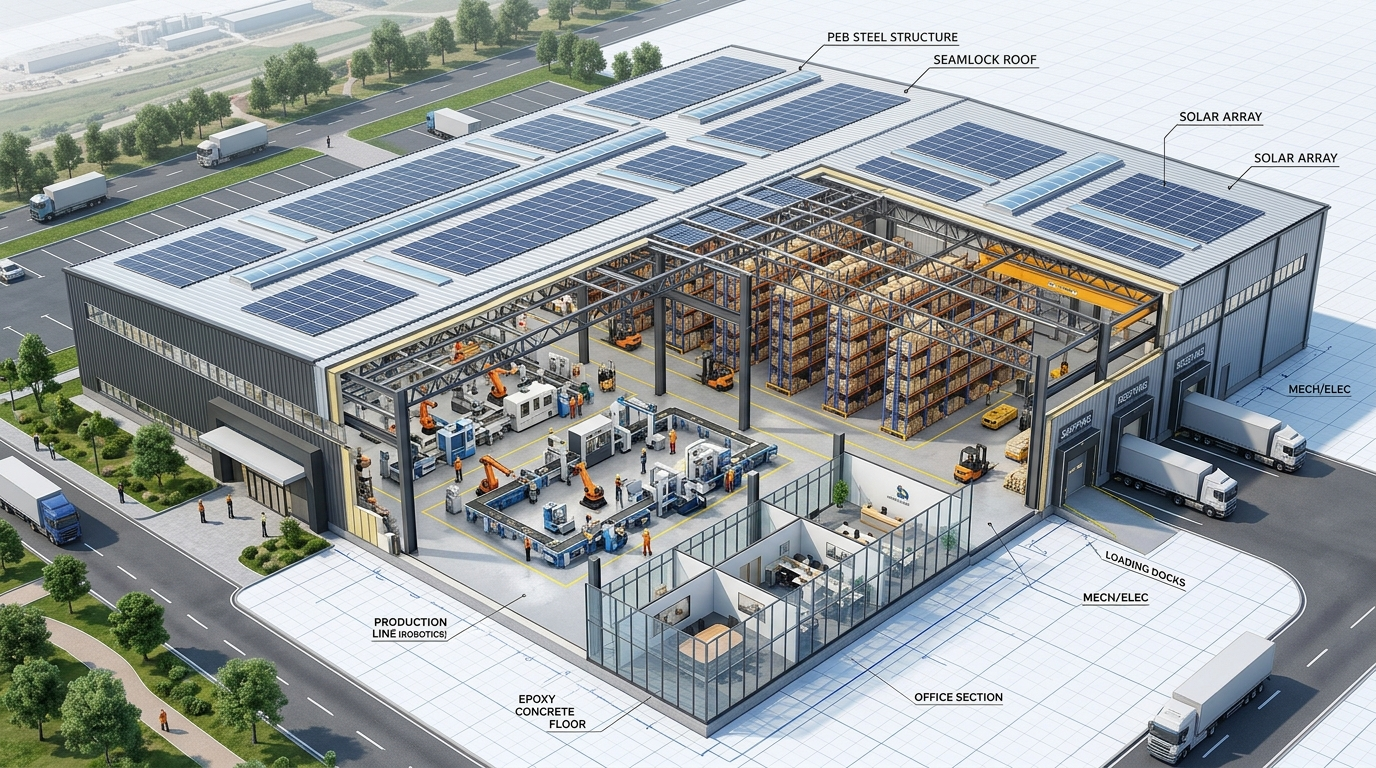
\includegraphics[height=118mm]{../../public/factory-tech-3d.jpg}};
  \fill[white, opacity=0.10] (0,0) rectangle (186,118);

  % Connectors
  \draw[TTCBlue!55!white, line width=0.65pt] (55,91) -- (80,72);
  \draw[TTCBlue!55!white, line width=0.65pt] (55,38) -- (81,57);
  \draw[TTCBlue!55!white, line width=0.65pt] (131,91) -- (107,72);
  \draw[TTCRed!72!white, line width=0.75pt] (131,38) -- (106,57);

  % 01 — AIDC ConTech
  \node[
    anchor=north west, rounded corners=3pt,
    fill=white, fill opacity=0.94, text opacity=1,
    draw=TTCCyan!70!white, line width=0.65pt,
    minimum width=53mm, minimum height=29mm,
    text width=47mm, inner sep=3mm, align=left
  ] at (5,113) {
    {\fontsize{7.3}{8.5}\selectfont\bfseries\color{TTCCyan} 01 / AIDC CONTECH}\\[1mm]
    {\fontsize{10}{11.5}\selectfont\bfseries\color{TTCBlue} BIM 5D • AI • 价值工程}\\[1mm]
    {\fontsize{7}{8.6}\selectfont\color{TTCTextDark}优化设计与数据模型，节省 10--15\% 投资成本。}
  };

  % 02 — MEP & PCCC
  \node[
    anchor=south west, rounded corners=3pt,
    fill=white, fill opacity=0.94, text opacity=1,
    draw=TTCBlue!42!white, line width=0.65pt,
    minimum width=53mm, minimum height=29mm,
    text width=47mm, inner sep=3mm, align=left
  ] at (5,5) {
    {\fontsize{7.3}{8.5}\selectfont\bfseries\color{TTCBlue} 02 / MEP 机电与消防}\\[1mm]
    {\fontsize{10}{11.5}\selectfont\bfseries\color{TTCBlue} 基于BIM的全专业协同}\\[1mm]
    {\fontsize{7}{8.6}\selectfont\color{TTCTextDark}电气、暖通、给排水与自动消防系统统一模型无缝集成。}
  };

  % 03 — Infrastructure
  \node[
    anchor=north east, rounded corners=3pt,
    fill=white, fill opacity=0.94, text opacity=1,
    draw=TTCBlue!42!white, line width=0.65pt,
    minimum width=53mm, minimum height=29mm,
    text width=47mm, inner sep=3mm, align=left
  ] at (181,113) {
    {\fontsize{7.3}{8.5}\selectfont\bfseries\color{TTCBlue} 03 / 园区配套基建}\\[1mm]
    {\fontsize{10}{11.5}\selectfont\bfseries\color{TTCBlue} 重载地基 • 道路 • 排水}\\[1mm]
    {\fontsize{7}{8.6}\selectfont\color{TTCTextDark}高标准园区基础设施，与厂区总平面布置完美对接。}
  };

  % 04 — PEB
  \node[
    anchor=south east, rounded corners=3pt,
    fill=white, fill opacity=0.96, text opacity=1,
    draw=TTCRed!78!white, line width=0.8pt,
    minimum width=53mm, minimum height=29mm,
    text width=47mm, inner sep=3mm, align=left
  ] at (181,5) {
    {\fontsize{7.3}{8.5}\selectfont\bfseries\color{TTCRed} 04 / PEB 钢结构制造}\\[1mm]
    {\fontsize{10}{11.5}\selectfont\bfseries\color{TTCBlue} 精密智造与品控}\\[1mm]
    {\fontsize{7}{8.6}\selectfont\color{TTCTextDark}CNC • SAW • AWS D1.1 • NDT；年供货能力达 30,000 吨。}
  };

  % Central hub
  \node[
    rounded corners=3pt, fill=TTCDeepNavy!96!black,
    draw=TTCCyan!75!white, line width=0.9pt,
    minimum width=50mm, minimum height=28mm,
    text=white, align=center, inner sep=2.5mm
  ] at (93,64) {
    {\fontsize{11}{12.5}\selectfont\bfseries 新成功 TTC}\\[1mm]
    {\fontsize{7.5}{9}\selectfont\bfseries\color{TTCCyan} EPC SYSTEM INTEGRATOR}\\[1mm]
    {\fontsize{6.8}{8}\selectfont\color{white!78!gray}One contract • One accountability}
  };

  \draw[white, line width=1.2pt, rounded corners=3pt] (0.6,0.6) rectangle (185.4,117.4);
  \draw[TTCBorder, line width=0.65pt, rounded corners=3pt] (0,0) rectangle (186,118);
\end{tikzpicture}

\vspace{3mm}

\noindent
\begin{tikzpicture}[x=1mm,y=1mm]
  \path[use as bounding box] (0,0) rectangle (186,31);
  \fill[TTCLightBlue, rounded corners=4pt] (0,0) rectangle (186,31);
  \draw[TTCBorder, line width=0.65pt, rounded corners=4pt] (0,0) rectangle (186,31);

  \node[align=center] at (18,15.5) {
    {\fontsize{7}{8}\selectfont\bfseries\color{TTCTextMuted} 01}\\[0.7mm]
    {\fontsize{9.2}{10.5}\selectfont\bfseries\color{TTCBlue} 现场勘察}\\[0.7mm]
    {\fontsize{6.6}{8}\selectfont 现状与需求分析}
  };
  \node[align=center] at (55.5,15.5) {
    {\fontsize{7}{8}\selectfont\bfseries\color{TTCTextMuted} 02}\\[0.7mm]
    {\fontsize{9.2}{10.5}\selectfont\bfseries\color{TTCBlue} 方案设计}\\[0.7mm]
    {\fontsize{6.6}{8}\selectfont BIM • AI • VE}
  };
  \node[align=center] at (93,15.5) {
    {\fontsize{7}{8}\selectfont\bfseries\color{TTCTextMuted} 03}\\[0.7mm]
    {\fontsize{9.2}{10.5}\selectfont\bfseries\color{TTCBlue} 基础工程}\\[0.7mm]
    {\fontsize{6.6}{8}\selectfont 地基与管网}
  };
  \node[align=center] at (130.5,15.5) {
    {\fontsize{7}{8}\selectfont\bfseries\color{TTCTextMuted} 04}\\[0.7mm]
    {\fontsize{9.2}{10.5}\selectfont\bfseries\color{TTCBlue} 机电与消防}\\[0.7mm]
    {\fontsize{6.6}{8}\selectfont 系统集成安装}
  };
  \node[align=center] at (168,15.5) {
    {\fontsize{7}{8}\selectfont\bfseries\color{TTCRed} 05}\\[0.7mm]
    {\fontsize{9.2}{10.5}\selectfont\bfseries\color{TTCRed} PEB制造}\\[0.7mm]
    {\fontsize{6.6}{8}\selectfont 构件加工与吊装}
  };

  \foreach \x in {36.75,74.25,111.75,149.25}{
    \node[text=TTCRed, font=\fontsize{8}{9}\selectfont] at (\x,15.5) {\faChevronRight};
  }
\end{tikzpicture}

\vspace{3mm}

\noindent
\begin{tabular}{@{}p{58mm}@{\hspace{6mm}}p{58mm}@{\hspace{6mm}}p{58mm}@{}}
  \begin{tikzpicture}
    \node[
      rounded corners=4pt, fill=white, draw=TTCBorder,
      line width=0.65pt, minimum width=58mm, minimum height=35mm,
      text width=50mm, inner sep=4mm, align=left
    ] {
      {\fontsize{7}{8}\selectfont\bfseries\color{TTCRed} 01 / ACCOUNTABILITY}\\[1mm]
      {\fontsize{14}{15.5}\selectfont\bfseries\color{TTCBlue} 01 责任总包}\\[1mm]
      {\fontsize{7}{8.5}\selectfont\color{TTCTextDark}单一总包主体对项目从设计到交付承担全过程责任。}
    };
  \end{tikzpicture}
  &
  \begin{tikzpicture}
    \node[
      rounded corners=4pt, fill=white, draw=TTCBorder,
      line width=0.65pt, minimum width=58mm, minimum height=35mm,
      text width=50mm, inner sep=4mm, align=left
    ] {
      {\fontsize{7}{8}\selectfont\bfseries\color{TTCCyan} 02 / OPTIMIZATION}\\[1mm]
      {\fontsize{14}{15.5}\selectfont\bfseries\color{TTCBlue} 成本优化}\\[1mm]
      {\fontsize{7}{8.5}\selectfont\color{TTCTextDark}AI与价值工程优化技术方案，节省10--15\%投资成本。}
    };
  \end{tikzpicture}
  &
  \begin{tikzpicture}
    \node[
      rounded corners=4pt, fill=white, draw=TTCBorder,
      line width=0.65pt, minimum width=58mm, minimum height=35mm,
      text width=50mm, inner sep=4mm, align=left
    ] {
      {\fontsize{7}{8}\selectfont\bfseries\color{TTCGold} 03 / RELIABILITY}\\[1mm]
      {\fontsize{14}{15.5}\selectfont\bfseries\color{TTCBlue} 100\% 按期交付}\\[1mm]
      {\fontsize{7}{8.5}\selectfont\color{TTCTextDark}自控重机与制造产能，保障项目关键节点绝对准时。}
    };
  \end{tikzpicture}
\end{tabular}
\end{minipage}
\newpage

% ============================================================
% TRANG 06: GOVERNANCE & COMPLIANCE DASHBOARD
% ============================================================
\pageheaderbar{组织架构与建设部二级资质认证}{第06页}
\pagefooterbar{第06页}

\begin{tikzpicture}[remember picture, overlay]
  \draw[TTCBlue!6!white, line width=0.45pt]
    ([xshift=15mm,yshift=18mm]current page.south west)
    grid[step=8mm]
    ([xshift=195mm,yshift=42mm]current page.south west);
\end{tikzpicture}

\begin{minipage}[t][246mm]{\textwidth}
\secbrand{精益治理与合规体系}{Governance Structure, Grade II Construction License \& International ISO Systems}

\vspace{1mm}
{\fontsize{15}{17}\selectfont\bfseries\color{TTCBlue}
权责分明 • 执行高效 • 全程闭环合规管理\par}
\vspace{1mm}
{\fontsize{7.5}{9}\selectfont\color{TTCTextMuted}
An execution-led governance model connecting board oversight directly to every project site.\par}
\vspace{3mm}

\noindent
\begin{tikzpicture}[x=1mm,y=1mm]
  \path[use as bounding box] (0,0) rectangle (186,105);
  \fill[white, rounded corners=4pt] (0,0) rectangle (186,105);
  \draw[TTCBorder, line width=0.7pt, rounded corners=4pt] (0,0) rectangle (186,105);

  \node[anchor=west, align=left] at (6,99) {
    {\fontsize{7}{8}\selectfont\bfseries\color{TTCCyan} DELIVERY GOVERNANCE}\\[-0.2mm]
    {\fontsize{9.5}{11}\selectfont\bfseries\color{TTCBlue} 矩阵式扁平化项目指挥与管理架构}
  };
  \draw[TTCBorder, line width=0.5pt] (6,91.5) -- (180,91.5);

  % Connectors
  \draw[TTCBlue!65!white, line width=0.75pt] (93,83) -- (93,75);
  \draw[TTCBlue!65!white, line width=0.75pt] (93,66) -- (93,61);
  \draw[TTCBlue!65!white, line width=0.75pt] (32,61) -- (154,61);
  \draw[TTCBlue!65!white, line width=0.75pt] (32,61) -- (32,57);
  \draw[TTCBlue!65!white, line width=0.75pt] (93,61) -- (93,57);
  \draw[TTCBlue!65!white, line width=0.75pt] (154,61) -- (154,57);
  \draw[TTCBlue!65!white, line width=0.75pt] (32,48) -- (32,43);
  \draw[TTCBlue!65!white, line width=0.75pt] (93,48) -- (93,43);
  \draw[TTCBlue!65!white, line width=0.75pt] (154,48) -- (154,43);
  \draw[TTCBlue!55!white, line width=0.65pt] (32,21) -- (32,16);
  \draw[TTCBlue!55!white, line width=0.65pt] (93,21) -- (93,16);
  \draw[TTCBlue!55!white, line width=0.65pt] (154,21) -- (154,16);
  \draw[TTCBlue!55!white, line width=0.65pt] (32,16) -- (154,16);
  \draw[TTCBlue!55!white, line width=0.65pt] (93,16) -- (93,13);
  \draw[TTCBlue!42!white, line width=0.6pt, dashed] (46,70.5) -- (62,70.5);
  \draw[TTCCyan!80!white, line width=0.6pt, dashed] (124,70.5) -- (140,70.5);

  % Board & executive
  \node[
    rounded corners=3pt, fill=TTCDeepNavy, text=white,
    minimum width=78mm, minimum height=10mm, align=center
  ] at (93,83) {
    {\fontsize{7.8}{9.2}\selectfont\bfseries
    \faUsers\quad 股东大会与董事会 (Board of Directors)}
  };
  \node[
    rounded corners=3pt, fill=TTCLightBlue, draw=TTCBorder,
    minimum width=42mm, minimum height=9mm, align=center
  ] at (25,70.5) {
    {\fontsize{7}{8.3}\selectfont\bfseries\color{TTCBlue} 国际工程专家顾问委员会}
  };
  \node[
    rounded corners=3pt, fill=TTCRed, text=white,
    minimum width=62mm, minimum height=11mm, align=center
  ] at (93,70.5) {
    {\fontsize{8.2}{9.5}\selectfont\bfseries
    \faUserTie\quad 总经理 (CEO)}\\[0.5mm]
    {\fontsize{6.7}{8}\selectfont 范辉新 (PHẠM HUY TÂN)}
  };
  \node[
    rounded corners=3pt, fill=TTCLightBlue, draw=TTCCyan,
    minimum width=42mm, minimum height=9mm, align=center
  ] at (161,70.5) {
    {\fontsize{7}{8.3}\selectfont\bfseries\color{TTCBlue}
    \faMicrochip\quad AIDC 建筑科技研发中心}
  };

  % Three executive streams
  \node[
    rounded corners=3pt, fill=TTCBlue, text=white,
    minimum width=54mm, minimum height=10mm, align=center
  ] at (32,52.5) {
    {\fontsize{7.4}{8.8}\selectfont\bfseries 项目工程副总经理 (COO)}
  };
  \node[
    rounded corners=3pt, fill=TTCBlue, text=white,
    minimum width=54mm, minimum height=10mm, align=center
  ] at (93,52.5) {
    {\fontsize{7.4}{8.8}\selectfont\bfseries 技术总工 \& BIM中心 (CTO)}
  };
  \node[
    rounded corners=3pt, fill=TTCBlue, text=white,
    minimum width=54mm, minimum height=10mm, align=center
  ] at (154,52.5) {
    {\fontsize{7.4}{8.8}\selectfont\bfseries 财务与商务合约副总 (CFO)}
  };

  % Functional teams
  \node[
    rounded corners=3pt, fill=white, draw=TTCBorder,
    minimum width=54mm, minimum height=22mm,
    text width=47mm, inner sep=3mm, align=left
  ] at (32,32) {
    {\fontsize{7.1}{8.4}\selectfont\bfseries\color{TTCBlue}\faHardHat\ PROJECT DELIVERY}\\[1mm]
    {\fontsize{6.7}{8.2}\selectfont\color{TTCTextDark}
    • FDI项目指挥部\\
    • 施工统筹与机械调度\\
    • 现场 HSE \& QA/QC 管控}
  };
  \node[
    rounded corners=3pt, fill=white, draw=TTCBorder,
    minimum width=54mm, minimum height=22mm,
    text width=47mm, inner sep=3mm, align=left
  ] at (93,32) {
    {\fontsize{7.1}{8.4}\selectfont\bfseries\color{TTCBlue}\faDraftingCompass\ ENGINEERING}\\[1mm]
    {\fontsize{6.7}{8.2}\selectfont\color{TTCTextDark}
    • 价值工程与结构优化\\
    • BIM 5D 与全生命周期数据\\
    • 规划、合规与消防审查}
  };
  \node[
    rounded corners=3pt, fill=white, draw=TTCBorder,
    minimum width=54mm, minimum height=22mm,
    text width=47mm, inner sep=3mm, align=left
  ] at (154,32) {
    {\fontsize{7.1}{8.4}\selectfont\bfseries\color{TTCBlue}\faFileInvoiceDollar\ COMMERCIAL}\\[1mm]
    {\fontsize{6.7}{8.2}\selectfont\color{TTCTextDark}
    • 招投标与FIDIC合同谈判\\
    • EPC现金流与资金风控\\
    • Tier-1 核心供应链采购}
  };

  % Site execution
  \node[
    rounded corners=3pt, fill=TTCDeepNavy, draw=TTCCyan,
    line width=0.75pt, text=white,
    minimum width=174mm, minimum height=12mm, align=center
  ] at (93,8) {
    {\fontsize{7.7}{9}\selectfont\bfseries\color{TTCCyan}
    \faHardHat\quad 现场项目指挥部 — 赋权一线，即时响应}\\[0.6mm]
    {\fontsize{6.5}{7.8}\selectfont\color{white!82!gray}
    项目经理 (PM) • 结构工程师 • MEP机电 • 常驻 HSE 与 QA/QC 工程师}
  };
\end{tikzpicture}

\vspace{3mm}

\noindent
\begin{tikzpicture}[x=1mm,y=1mm]
  \path[use as bounding box] (0,0) rectangle (186,72);
  \fill[TTCLightBlue, rounded corners=4pt] (0,0) rectangle (186,72);
  \draw[TTCBorder, line width=0.7pt, rounded corners=4pt] (0,0) rectangle (186,72);

  \node[anchor=west, align=left] at (6,66) {
    {\fontsize{7}{8}\selectfont\bfseries\color{TTCCyan} COMPLIANCE PASSPORT}\\[-0.2mm]
    {\fontsize{9.5}{11}\selectfont\bfseries\color{TTCBlue}
    法定资质与国际化质量认证体系}
  };

  % Grade II card
  \fill[white, rounded corners=3pt] (5,7) rectangle (58,57);
  \draw[TTCRed, line width=0.9pt, rounded corners=3pt] (5,7) rectangle (58,57);
  \node[align=center] at (31.5,45) {
    {\fontsize{7}{8}\selectfont\bfseries\color{TTCRed} CONSTRUCTION LICENSE}\\[1mm]
    {\fontsize{20}{22}\selectfont\bfseries\color{TTCRed} 二级资质}\\[-0.2mm]
    {\fontsize{8.5}{10}\selectfont\bfseries\color{TTCBlue} 越南建设部颁发}
  };
  \draw[TTCBorder, line width=0.5pt] (11,29) -- (52,29);
  \node[text width=42mm, align=left] at (31.5,18) {
    {\fontsize{6.6}{8.2}\selectfont\color{TTCTextDark}
    \textcolor{TTCRed}{\faCheckCircle}\ 工业建筑设计与施工总承包\\
    \textcolor{TTCRed}{\faCheckCircle}\ 无建筑面积与楼层上限限制\\
    \textcolor{TTCRed}{\faCheckCircle}\ 超大跨度重型工业厂房资质}
  };

  % ISO 9001
  \fill[white, rounded corners=3pt] (62,7) rectangle (100,57);
  \draw[TTCBorder, line width=0.6pt, rounded corners=3pt] (62,7) rectangle (100,57);
  \node[align=center] at (81,45) {
    {\fontsize{7}{8}\selectfont\bfseries\color{TTCCyan} QUALITY}\\[1mm]
    {\fontsize{13}{14.5}\selectfont\bfseries\color{TTCBlue} ISO 9001}\\
    {\fontsize{7}{8.5}\selectfont\bfseries\color{TTCTextMuted} 2015}
  };
  \node[text width=30mm, align=center] at (81,20) {
    {\fontsize{6.6}{8.2}\selectfont\color{TTCTextDark}
    全流程质量管理，材料、施工及验收执行4层ITP标准。}
  };

  % ISO 14001
  \fill[white, rounded corners=3pt] (103,7) rectangle (141,57);
  \draw[TTCBorder, line width=0.6pt, rounded corners=3pt] (103,7) rectangle (141,57);
  \node[align=center] at (122,45) {
    {\fontsize{7}{8}\selectfont\bfseries\color{TTCCyan} ENVIRONMENT}\\[1mm]
    {\fontsize{13}{14.5}\selectfont\bfseries\color{TTCBlue} ISO 14001}\\
    {\fontsize{7}{8.5}\selectfont\bfseries\color{TTCTextMuted} 2015}
  };
  \node[text width=30mm, align=center] at (122,20) {
    {\fontsize{6.6}{8.2}\selectfont\color{TTCTextDark}
    环境管理体系，严控废弃物与噪音，优先低碳建造方案。}
  };

  % ISO 45001
  \fill[white, rounded corners=3pt] (144,7) rectangle (182,57);
  \draw[TTCGold, line width=0.75pt, rounded corners=3pt] (144,7) rectangle (182,57);
  \node[align=center] at (163,45) {
    {\fontsize{7}{8}\selectfont\bfseries\color{TTCGold} HEALTH \& SAFETY}\\[1mm]
    {\fontsize{13}{14.5}\selectfont\bfseries\color{TTCBlue} ISO 45001}\\
    {\fontsize{7}{8.5}\selectfont\bfseries\color{TTCTextMuted} 2018}
  };
  \node[text width=30mm, align=center] at (163,20) {
    {\fontsize{6.6}{8.2}\selectfont\color{TTCTextDark}
    职业健康安全体系，坚持零事故政策与全员安全培训。}
  };
\end{tikzpicture}

\vspace{3mm}

\noindent
\begin{tikzpicture}[x=1mm,y=1mm]
  \path[use as bounding box] (0,0) rectangle (186,24);
  \fill[white, rounded corners=4pt] (0,0) rectangle (186,24);
  \draw[TTCBorder, line width=0.7pt, rounded corners=4pt] (0,0) rectangle (186,24);
  \fill[TTCDeepNavy, rounded corners=4pt] (0,0) rectangle (47,24);
  \node[align=left, anchor=west] at (6,12) {
    {\fontsize{7}{8}\selectfont\bfseries\color{TTCCyan} PRE-QUALIFICATION}\\[0.8mm]
    {\fontsize{10}{11.5}\selectfont\bfseries\color{white} READY FOR FDI}\\[0.5mm]
    {\fontsize{6.3}{7.6}\selectfont\color{white!72!gray}Legal • Quality • HSE}
  };
  \node[align=center] at (72,12) {
    {\fontsize{11}{12.5}\selectfont\bfseries\color{TTCBlue} 01}\\[0.6mm]
    {\fontsize{7}{8.3}\selectfont\bfseries\color{TTCTextDark} 一站式法人责任}
  };
  \node[align=center] at (113,12) {
    {\fontsize{11}{12.5}\selectfont\bfseries\color{TTCBlue} 04}\\[0.6mm]
    {\fontsize{7}{8.3}\selectfont\bfseries\color{TTCTextDark} 4级 ITP 品控体系}
  };
  \node[align=center] at (160,12) {
    {\fontsize{11}{12.5}\selectfont\bfseries\color{TTCRed} 100\%}\\[0.6mm]
    {\fontsize{7}{8.3}\selectfont\bfseries\color{TTCTextDark} CO/CQ 材料溯源}
  };
\end{tikzpicture}
\end{minipage}
\newpage

% ============================================================
% TRANG 07: NĂNG LỰC NHÂN SỰ TRIỂN KHAI EPC
% ============================================================
\pageheaderbar{EPC项目实施人力资源能力}{第07页}
\pagefooterbar{第07页}

\begin{tikzpicture}[remember picture, overlay]
  \draw[TTCBlue!6!white, line width=0.45pt]
    ([xshift=15mm,yshift=18mm]current page.south west)
    grid[step=8mm]
    ([xshift=195mm,yshift=42mm]current page.south west);
\end{tikzpicture}

\begin{minipage}[t][246mm]{\textwidth}
\secbrand{全生命周期集成化项目团队}{Integrated Project Team, Clear Accountability \& Site-Ready Mobilization}

\vspace{1mm}
{\fontsize{15}{17}\selectfont\bfseries\color{TTCBlue}
合适的人选 • 明确的角色 • 精准的时机\par}
\vspace{1mm}
{\fontsize{7.5}{9}\selectfont\color{TTCTextMuted}
One accountable team mobilized from pre-construction through commissioning and warranty.\par}
\vspace{3mm}

\noindent
\begin{tikzpicture}[x=1mm,y=1mm]
  \path[use as bounding box] (0,0) rectangle (186,72);
  \clip[rounded corners=3pt] (0,0) rectangle (186,72);
  \node[anchor=center, inner sep=0pt] at (93,36)
    {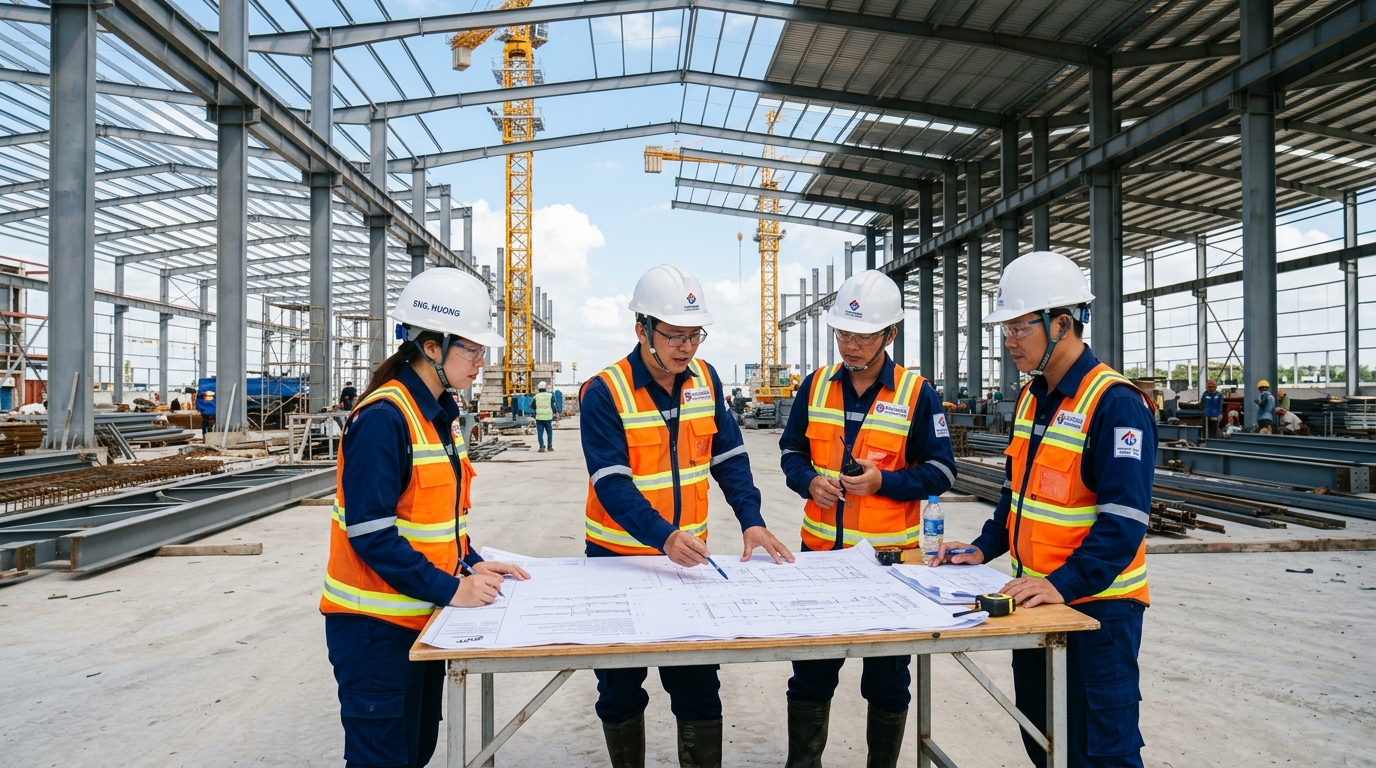
\includegraphics[width=186mm]{../../public/engineer-team-site.jpg}};
  \fill[TTCDeepNavy, opacity=0.82] (0,0) rectangle (68,72);
  \fill[TTCDeepNavy, opacity=0.38] (68,0) rectangle (92,72);

  \node[anchor=west, text width=54mm, align=left, text=white] at (8,48) {
    {\fontsize{7}{8}\selectfont\bfseries\color{TTCCyan} PEOPLE AT THE POINT OF EXECUTION}\\[1.5mm]
    {\fontsize{15}{17}\selectfont\bfseries 现场执行一线的\\专业力量}\\[2mm]
    {\fontsize{7.2}{9}\selectfont\color{white!84!gray}
    项目团队按任务单元编制，职权清晰明确，执行单一指挥线的高效汇报机制。}
  };

  \node[
    anchor=south east, rounded corners=3pt,
    fill=white, fill opacity=0.93, text opacity=1,
    draw=TTCCyan, line width=0.7pt,
    minimum width=52mm, minimum height=14mm, align=center
  ] at (179,7) {
    {\fontsize{8}{9.5}\selectfont\bfseries\color{TTCBlue} FIELD-LED DECISION MAKING}\\[0.7mm]
    {\fontsize{6.5}{8}\selectfont\color{TTCTextDark}技术与管理决策直接贴近施工现场一线}
  };
  \draw[white, line width=1pt, rounded corners=3pt] (0.6,0.6) rectangle (185.4,71.4);
  \draw[TTCBorder, line width=0.65pt, rounded corners=3pt] (0,0) rectangle (186,72);
\end{tikzpicture}

\vspace{3mm}

\noindent
\begin{tikzpicture}[x=1mm,y=1mm]
  \path[use as bounding box] (0,0) rectangle (186,67);
  \node[anchor=west, align=left] at (0,62) {
    {\fontsize{7}{8}\selectfont\bfseries\color{TTCCyan} PROJECT TEAM BY PHASE}\quad
    {\fontsize{9.5}{11}\selectfont\bfseries\color{TTCBlue} 项目各阶段核心责任角色分工}
  };

  % Phase 01
  \fill[white, rounded corners=3pt] (0,0) rectangle (58,55);
  \draw[TTCBorder, line width=0.65pt, rounded corners=3pt] (0,0) rectangle (58,55);
  \fill[TTCLightBlue, rounded corners=3pt] (0,43) rectangle (58,55);
  \node[anchor=west] at (5,49) {
    {\fontsize{7}{8}\selectfont\bfseries\color{TTCCyan} 01 / PRE-CONSTRUCTION}
  };
  \node[anchor=north west, text width=48mm, align=left] at (5,39) {
    {\fontsize{9.5}{11}\selectfont\bfseries\color{TTCBlue} 前期准备与设计}\\[1.2mm]
    {\fontsize{7}{8.6}\selectfont\color{TTCTextDark}
    \textbf{Project Director}\\
    与业主对接的单一总责任人。\\[0.8mm]
    \textbf{Design \& BIM Lead}\\
    设计统筹、价值工程与模型深化。\\[0.8mm]
    \textbf{Planning / QS / FIDIC}\\
    锁定工程范围、进度总计划与预算。}
  };
  \node[anchor=south, align=center] at (29,3.5) {
    {\fontsize{6.5}{7.8}\selectfont\bfseries\color{TTCRed} OUTPUT: APPROVED BASELINE}
  };

  % Phase 02
  \fill[white, rounded corners=3pt] (64,0) rectangle (122,55);
  \draw[TTCBlue!55!white, line width=0.75pt, rounded corners=3pt] (64,0) rectangle (122,55);
  \fill[TTCBlue, rounded corners=3pt] (64,43) rectangle (122,55);
  \node[anchor=west] at (69,49) {
    {\fontsize{7}{8}\selectfont\bfseries\color{white} 02 / CONSTRUCTION}
  };
  \node[anchor=north west, text width=48mm, align=left] at (69,39) {
    {\fontsize{9.5}{11}\selectfont\bfseries\color{TTCBlue} 现场施工装配}\\[1.2mm]
    {\fontsize{7}{8.6}\selectfont\color{TTCTextDark}
    \textbf{Construction / Site Manager}\\
    资源调配 • 作业面统筹 • 施工班组。\\[0.5mm]
    \textbf{Discipline Engineers}\\
    结构 • 园区基建 • MEP • 消防。\\[0.5mm]
    \textbf{HSE \& QA/QC Managers}\\
    独立行使安全与质量一票否决权。}
  };
  \node[anchor=south, align=center] at (93,2.5) {
    {\fontsize{6.5}{7.8}\selectfont\bfseries\color{TTCRed} OUTPUT: CONTROLLED EXECUTION}
  };

  % Phase 03
  \fill[white, rounded corners=3pt] (128,0) rectangle (186,55);
  \draw[TTCBorder, line width=0.65pt, rounded corners=3pt] (128,0) rectangle (186,55);
  \fill[TTCLightBlue, rounded corners=3pt] (128,43) rectangle (186,55);
  \node[anchor=west] at (133,49) {
    {\fontsize{7}{8}\selectfont\bfseries\color{TTCCyan} 03 / HANDOVER \& O\&M}
  };
  \node[anchor=north west, text width=48mm, align=left] at (133,39) {
    {\fontsize{9.5}{11}\selectfont\bfseries\color{TTCBlue} 竣工交付与运维}\\[1.2mm]
    {\fontsize{7}{8.6}\selectfont\color{TTCTextDark}
    \textbf{Commissioning Manager}\\
    统筹系统联合调试与试运行。\\[0.8mm]
    \textbf{As-built \& Digital Twin Team}\\
    标准化竣工图纸与数字资产交付。\\[0.8mm]
    \textbf{Warranty Response Team}\\
    24/7 快速技术支持与质保服务。}
  };
  \node[anchor=south, align=center] at (157,3.5) {
    {\fontsize{6.5}{7.8}\selectfont\bfseries\color{TTCRed} OUTPUT: READY FOR OPERATION}
  };
\end{tikzpicture}

\vspace{3mm}

\noindent
\begin{tikzpicture}[x=1mm,y=1mm]
  \path[use as bounding box] (0,0) rectangle (186,29);
  \fill[TTCLightBlue, rounded corners=4pt] (0,0) rectangle (186,29);
  \draw[TTCBorder, line width=0.65pt, rounded corners=4pt] (0,0) rectangle (186,29);

  \node[align=center] at (22,14.5) {
    {\fontsize{6.5}{7.8}\selectfont\bfseries\color{TTCTextMuted} GOVERNANCE}\\[0.7mm]
    {\fontsize{9.2}{10.5}\selectfont\bfseries\color{TTCBlue} 总部 PMO}\\[0.5mm]
    {\fontsize{6.4}{7.6}\selectfont 项目组合管控}
  };
  \node[text=TTCRed] at (45,14.5) {\faChevronRight};
  \node[align=center] at (68,14.5) {
    {\fontsize{6.5}{7.8}\selectfont\bfseries\color{TTCTextMuted} ACCOUNTABILITY}\\[0.7mm]
    {\fontsize{9.2}{10.5}\selectfont\bfseries\color{TTCBlue} 项目总监}\\[0.5mm]
    {\fontsize{6.4}{7.6}\selectfont 单一责任主体}
  };
  \node[text=TTCRed] at (93,14.5) {\faChevronRight};
  \node[align=center] at (118,14.5) {
    {\fontsize{6.5}{7.8}\selectfont\bfseries\color{TTCTextMuted} SITE AUTHORITY}\\[0.7mm]
    {\fontsize{9.2}{10.5}\selectfont\bfseries\color{TTCBlue} 现场指挥部}\\[0.5mm]
    {\fontsize{6.4}{7.6}\selectfont 一线执行决策}
  };
  \node[text=TTCRed] at (141,14.5) {\faChevronRight};
  \node[align=center] at (164,14.5) {
    {\fontsize{6.5}{7.8}\selectfont\bfseries\color{TTCTextMuted} DELIVERY}\\[0.7mm]
    {\fontsize{9.2}{10.5}\selectfont\bfseries\color{TTCRed} 专业施工班组}\\[0.5mm]
    {\fontsize{6.4}{7.6}\selectfont 专业任务交付}
  };
\end{tikzpicture}

\vspace{3mm}

\noindent
\begin{tikzpicture}[x=1mm,y=1mm]
  \path[use as bounding box] (0,0) rectangle (186,27);
  \fill[white, rounded corners=4pt] (0,0) rectangle (186,27);
  \draw[TTCBorder, line width=0.65pt, rounded corners=4pt] (0,0) rectangle (186,27);
  \foreach \x in {46.5,93,139.5}{
    \draw[TTCBorder, line width=0.5pt] (\x,5) -- (\x,22);
  }
  \node[align=center] at (23.25,13.5) {
    {\fontsize{14}{15.5}\selectfont\bfseries\color{TTCRed} 350+}\\[0.8mm]
    {\fontsize{6.8}{8}\selectfont\bfseries\color{TTCTextDark} 管理人员与工程师}
  };
  \node[align=center] at (69.75,13.5) {
    {\fontsize{14}{15.5}\selectfont\bfseries\color{TTCBlue} 2,500+}\\[0.8mm]
    {\fontsize{6.8}{8}\selectfont\bfseries\color{TTCTextDark} 专业技术工人}
  };
  \node[align=center] at (116.25,13.5) {
    {\fontsize{14}{15.5}\selectfont\bfseries\color{TTCCyan} 85+}\\[0.8mm]
    {\fontsize{6.8}{8}\selectfont\bfseries\color{TTCTextDark} 注册监理与施工队长}
  };
  \node[align=center] at (162.75,13.5) {
    {\fontsize{14}{15.5}\selectfont\bfseries\color{TTCBlue} 60+}\\[0.8mm]
    {\fontsize{6.8}{8}\selectfont\bfseries\color{TTCTextDark} BIM与数字化专家}
  };
\end{tikzpicture}
\end{minipage}
\newpage

% ============================================================
% TRANG 08: QUẢN TRỊ TÀI CHÍNH DỰ ÁN & KỶ LUẬT DÒNG TIỀN
% ============================================================
\pageheaderbar{项目财务管理与现金流纪律}{第08页}
\pagefooterbar{第08页}

\begin{tikzpicture}[remember picture, overlay]
  \node[opacity=0.025, scale=2.6, font=\bfseries\sffamily, text=TTCBlue]
    at ([yshift=-12mm]current page.center) {FINANCIAL GOVERNANCE \& DISCIPLINE};
  \draw[TTCBlue!6!white, line width=0.45pt]
    ([xshift=15mm, yshift=20mm]current page.south west)
    grid[step=8mm]
    ([xshift=195mm, yshift=45mm]current page.south west);
\end{tikzpicture}

\begin{minipage}[t][246mm]{\textwidth}
\secbrand{项目财务管理与现金流纪律}{Project Financial Governance • Cost Discipline • Verified \& Traceable Records}

\vspace{1mm}
{\fontsize{14.5}{16.5}\selectfont\bfseries\color{TTCBlue}
从投标决策到竣工结算的全流程闭环资金风控\par}
\vspace{1mm}
{\fontsize{7.5}{9}\selectfont\color{TTCTextMuted}
每个工程均设立独立核算代码，严格执行四道管控关口与定期财务对账，确保资金安全与履约保障。\par}
\vspace{3.5mm}

\noindent
\begin{tikzpicture}[x=1mm,y=1mm]
  \path[use as bounding box] (0,0) rectangle (186,86);

  % KHỐI TRÁI: 4 CỔNG KIỂM SOÁT
  \fill[white, rounded corners=4pt] (0,0) rectangle (126,86);
  \draw[TTCBorder, line width=0.7pt, rounded corners=4pt] (0,0) rectangle (126,86);

  \node[anchor=west, text=TTCCyan, font=\fontsize{7}{8}\selectfont\bfseries]
    at (6,79.5) {FOUR FINANCIAL CONTROL GATES};
  \node[anchor=west, text=TTCBlue, font=\fontsize{10}{12}\selectfont\bfseries]
    at (6,72.5) {项目财务四道管控关口体系};

  % Timeline connector bar
  \draw[TTCBlue!30!white, line width=1pt] (15,50) -- (111,50);

  % Cổng 01
  \fill[TTCRed] (15,50) circle (4.8);
  \node[text=white, font=\fontsize{7}{8}\selectfont\bfseries] at (15,50) {01};
  \node[anchor=south, align=center, text width=26mm, text=TTCRed, font=\fontsize{7}{8.2}\selectfont\bfseries]
    at (15,57.5) {合同审查\\与风险评估};
  \node[anchor=north, align=center, text width=27mm, text=TTCTextDark, font=\fontsize{6.2}{7.6}\selectfont]
    at (15,42.5) {毛利率底线测算\\支付与结算条款\\质保与违约风险};

  % Cổng 02
  \fill[white] (47,50) circle (4.8);
  \draw[TTCBlue, line width=0.85pt] (47,50) circle (4.8);
  \node[text=TTCBlue, font=\fontsize{7}{8}\selectfont\bfseries] at (47,50) {02};
  \node[anchor=south, align=center, text width=26mm, text=TTCBlue, font=\fontsize{7}{8.2}\selectfont\bfseries]
    at (47,57.5) {项目基准\\预算锁定};
  \node[anchor=north, align=center, text width=27mm, text=TTCTextDark, font=\fontsize{6.2}{7.6}\selectfont]
    at (47,42.5) {WBS目标成本基准\\阶段现金流计划\\物资支付限额锁定};

  % Cổng 03
  \fill[white] (79,50) circle (4.8);
  \draw[TTCBlue, line width=0.85pt] (79,50) circle (4.8);
  \node[text=TTCBlue, font=\fontsize{7}{8}\selectfont\bfseries] at (79,50) {03};
  \node[anchor=south, align=center, text width=26mm, text=TTCBlue, font=\fontsize{7}{8.2}\selectfont\bfseries]
    at (79,57.5) {过程执行\\动态监控};
  \node[anchor=north, align=center, text width=27mm, text=TTCTextDark, font=\fontsize{6.2}{7.6}\selectfont]
    at (79,42.5) {周度成本偏差分析\\工程变更(VO)审批\\竣工成本预测(EAC)};

  % Cổng 04
  \fill[white] (111,50) circle (4.8);
  \draw[TTCBlue, line width=0.85pt] (111,50) circle (4.8);
  \node[text=TTCBlue, font=\fontsize{7}{8}\selectfont\bfseries] at (111,50) {04};
  \node[anchor=south, align=center, text width=26mm, text=TTCBlue, font=\fontsize{7}{8.2}\selectfont\bfseries]
    at (111,57.5) {竣工验收\\与财务决算};
  \node[anchor=north, align=center, text width=27mm, text=TTCTextDark, font=\fontsize{6.2}{7.6}\selectfont]
    at (111,42.5) {竣工工程量档案\\应收账款回收清盘\\关闭项目成本账户};

  % Dải cam kết phía dưới khối trái
  \fill[TTCDeepNavy, rounded corners=3pt] (5,5.5) rectangle (121,18.5);
  \node[anchor=west, text=TTCCyan, font=\fontsize{6.8}{8}\selectfont\bfseries]
    at (8,12) {\faShield*\quad CONTROL BEFORE COMMITMENT};
  \node[anchor=east, text=white, font=\fontsize{6.5}{7.8}\selectfont\bfseries]
    at (118,12) {预算未定不立项，现金流不稳不调配};

  % KHỐI PHẢI: NGUYÊN TẮC QUẢN TRỊ
  \fill[TTCLightBlue, rounded corners=4pt] (131,0) rectangle (186,86);
  \draw[TTCBorder, line width=0.7pt, rounded corners=4pt] (131,0) rectangle (186,86);

  \node[anchor=north west, text=TTCCyan, font=\fontsize{7}{8}\selectfont\bfseries]
    at (136,79.5) {CONTROL PRINCIPLE};
  \node[anchor=north west, text width=46mm, text=TTCBlue, font=\fontsize{9.5}{11.5}\selectfont\bfseries]
    at (136,73) {严禁超能力盲目承揽};
  \fill[TTCRed] (136,61.5) rectangle (152,63);

  \node[anchor=north west, text width=45mm, text=TTCTextDark, font=\fontsize{6.8}{8.6}\selectfont]
    at (136,56) {
    \textcolor{TTCRed}{\faCheckCircle}\ \textbf{预算锁定：} 调配资源前 100\% 锁定成本基准。\\[2.4mm]
    \textcolor{TTCRed}{\faCheckCircle}\ \textbf{变更受控：} 额外支出必须有对应资金来源弥补。\\[2.4mm]
    \textcolor{TTCRed}{\faCheckCircle}\ \textbf{安全扩张：} 唯有保障交付与现金流方可拓展新单。
  };

  \fill[white, rounded corners=2.5pt, draw=TTCBorder, line width=0.55pt] (136,6) rectangle (181,18);
  \node[anchor=center, text=TTCBlue, font=\fontsize{6.6}{8}\selectfont\bfseries, align=center]
    at (158.5,12) {\faLock\quad 100\% 项目实行独立财务代码};
\end{tikzpicture}

\vspace{3.5mm}

\noindent
\begin{tikzpicture}[x=1mm,y=1mm]
  \path[use as bounding box] (0,0) rectangle (186,58);

  % Card 1: Cost Control
  \fill[white, rounded corners=4pt] (0,0) rectangle (58,58);
  \draw[TTCBorder, line width=0.65pt, rounded corners=4pt] (0,0) rectangle (58,58);
  \fill[TTCRed, rounded corners=1pt] (5,50.5) rectangle (22,52.5);
  \node[anchor=north west, text width=50mm, align=left] at (5,47.5) {
    {\fontsize{7}{8.2}\selectfont\bfseries\color{TTCRed}\faCalculator\quad COST CONTROL}\\[1.2mm]
    {\fontsize{9.8}{11.5}\selectfont\bfseries\color{TTCBlue} 成本动态精控}\\[2mm]
    {\fontsize{6.6}{8.2}\selectfont\color{TTCTextDark}
    \textbullet\ 按WBS建立基准预算 (Baseline)。\newline
    \textbullet\ 周度对比与成本偏差追踪预警。\newline
    \textbullet\ 完工总成本预测模型 (EAC)。}
  };

  % Card 2: Receivable Control
  \fill[white, rounded corners=4pt] (64,0) rectangle (122,58);
  \draw[TTCBorder, line width=0.65pt, rounded corners=4pt] (64,0) rectangle (122,58);
  \fill[TTCCyan, rounded corners=1pt] (69,50.5) rectangle (86,52.5);
  \node[anchor=north west, text width=50mm, align=left] at (69,47.5) {
    {\fontsize{7}{8.2}\selectfont\bfseries\color{TTCCyan}\faFileInvoiceDollar\quad RECEIVABLE CONTROL}\\[1.2mm]
    {\fontsize{9.8}{11.5}\selectfont\bfseries\color{TTCBlue} 账款严密管控}\\[2mm]
    {\fontsize{6.6}{8.2}\selectfont\color{TTCTextDark}
    \textbullet\ 紧跟4级ITP检验批节点请款。\newline
    \textbullet\ 实时监控预付款与工程进度款。\newline
    \textbullet\ 质保金与供应链付款全周期联动。}
  };

  % Card 3: Verified Reporting
  \fill[white, rounded corners=4pt] (128,0) rectangle (186,58);
  \draw[TTCBorder, line width=0.65pt, rounded corners=4pt] (128,0) rectangle (186,58);
  \fill[TTCBlue, rounded corners=1pt] (133,50.5) rectangle (150,52.5);
  \node[anchor=north west, text width=50mm, align=left] at (133,47.5) {
    {\fontsize{7}{8.2}\selectfont\bfseries\color{TTCBlue}\faClipboardCheck\quad VERIFIED REPORTING}\\[1.2mm]
    {\fontsize{9.8}{11.5}\selectfont\bfseries\color{TTCBlue} 溯源核验档案}\\[2mm]
    {\fontsize{6.6}{8.2}\selectfont\color{TTCTextDark}
    \textbullet\ 项目成本数据实时云端同步。\newline
    \textbullet\ 符合国际标准的管理会计月报。\newline
    \textbullet\ 随时接受业主委托独立三方审计。}
  };
\end{tikzpicture}

\vspace{3.5mm}

\noindent
\begin{tikzpicture}[x=1mm,y=1mm]
  \path[use as bounding box] (0,0) rectangle (186,46);

  % Outer Card
  \fill[white, rounded corners=4pt] (0,0) rectangle (186,46);
  \draw[TTCBorder, line width=0.65pt, rounded corners=4pt] (0,0) rectangle (186,46);

  % Left Navy Brand Anchor
  \fill[TTCDeepNavy, rounded corners=4pt] (0,0) rectangle (48,46);
  \node[anchor=west, text width=40mm, align=left] at (6,23) {
    {\fontsize{7}{8}\selectfont\bfseries\color{TTCCyan} DISCLOSURE POLICY}\\[1.2mm]
    {\fontsize{9}{11}\selectfont\bfseries\color{white} 受控透明与\\合规披露}\\[1.8mm]
    {\fontsize{6}{7.2}\selectfont\color{white!75!gray}Verified data \textbullet\ Right audience}
  };

  % 4 Pill Cards
  \foreach \xa/\xb/\num/\label/\sub in {
    53/81/01/财务审计报告/独立三方审计,
    85/113/02/完税证明文件/依法足额纳税,
    117/145/03/供应链往来对账/0 供应商欠款,
    149/181/04/项目管理报告/透明现金流跟踪}{
    \fill[TTCLightBlue, rounded corners=3pt] (\xa,14) rectangle (\xb,40);
    \draw[TTCBorder, line width=0.5pt, rounded corners=3pt] (\xa,14) rectangle (\xb,40);
    \node[text=TTCRed, font=\fontsize{8}{9.5}\selectfont\bfseries] at ({(\xa+\xb)/2},34.5) {\num};
    \node[align=center, text width=26mm, text=TTCBlue, font=\fontsize{6.5}{7.8}\selectfont\bfseries]
      at ({(\xa+\xb)/2},26) {\label};
    \node[align=center, text width=26mm, text=TTCTextMuted, font=\fontsize{5.8}{7}\selectfont]
      at ({(\xa+\xb)/2},18.5) {\sub};
  }

  % Bottom Notice
  \draw[TTCBorder, line width=0.5pt] (53,9.5) -- (181,9.5);
  \node[anchor=south west, text=TTCTextMuted, font=\fontsize{6}{7.3}\selectfont\itshape]
    at (53,3) {\faLock\quad 详细财务与税务数据可在招标阶段或签署双向保密协议 (NDA) 后正式提供。};
\end{tikzpicture}
\end{minipage}
\newpage

% ============================================================
% TRANG 09: NĂNG LỰC HUY ĐỘNG CHO DỰ ÁN EPC
% ============================================================
\pageheaderbar{银行信用额度与精英团队保障}{第09页}
\pagefooterbar{第09页}

\begin{tikzpicture}[remember picture, overlay]
  \node[opacity=0.02, scale=2.4, font=\bfseries\sffamily, text=TTCBlue]
    at ([yshift=-12mm]current page.center) {BANKING CAPACITY \& SITE MOBILIZATION};
  \draw[TTCBlue!6!white, line width=0.45pt]
    ([xshift=15mm, yshift=20mm]current page.south west)
    grid[step=8mm]
    ([xshift=195mm, yshift=45mm]current page.south west);
\end{tikzpicture}

\begin{minipage}[t][246mm]{\textwidth}
\secbrand{EPC项目履约保障能力}{Banking Capacity, Performance Bonds \& Site-Ready Workforce Mobilization}

\vspace{1mm}
{\fontsize{14.5}{16.5}\selectfont\bfseries\color{TTCBlue}
双重履约引擎 • 资金授信与实战团队全面就绪\par}
\vspace{1mm}
{\fontsize{7.5}{9}\selectfont\color{TTCTextMuted}
雄厚银行信贷额度支撑结合多兵种实战型技术队伍，按合同节点即时响应并高效推进。\par}
\vspace{3.5mm}

\noindent
\begin{tikzpicture}[x=1mm,y=1mm]
  \path[use as bounding box] (0,0) rectangle (186,80);

  % KHỐI TRÁI: FINANCIAL ENGINE
  \fill[white, rounded corners=4pt] (0,0) rectangle (90,80);
  \draw[TTCBorder, line width=0.7pt, rounded corners=4pt] (0,0) rectangle (90,80);

  \node[anchor=north west, text=TTCCyan, font=\fontsize{7}{8}\selectfont\bfseries]
    at (6,73.5) {FINANCIAL ENGINE};
  \node[anchor=north west, text=TTCBlue, font=\fontsize{10}{12}\selectfont\bfseries]
    at (6,67) {银行授信与履约保函能力};

  \node[anchor=west] at (6,54) {
    {\fontsize{23}{25}\selectfont\bfseries\color{TTCRed} 2500 亿越盾}\quad
    {\fontsize{7.5}{9}\selectfont\bfseries\color{TTCTextMuted} 银行总授信额度}
  };

  % Bank Badges
  \fill[TTCLightBlue, rounded corners=2.5pt, draw=TTCBorder, line width=0.5pt] (5,38) rectangle (85,46);
  \node[anchor=center, text=TTCBlue, font=\fontsize{6.2}{7.4}\selectfont\bfseries]
    at (45,42) {Vietcombank \textbullet\ BIDV \textbullet\ VietinBank \textbullet\ TPBank \textbullet\ ACB \textbullet\ MB};

  \node[anchor=north west, text width=80mm, text=TTCTextDark, font=\fontsize{6.8}{8.6}\selectfont]
    at (6,33.5) {
    \textcolor{TTCRed}{\faCheckCircle}\ \textbf{全类型保函：} 投标保函、履约保函、预付款保函与质保函。\\[1.4mm]
    \textcolor{TTCRed}{\faCheckCircle}\ \textbf{快速出函：} 满足条件后 24--48 小时内开具主流银行保函。\\[1.4mm]
    \textcolor{TTCRed}{\faCheckCircle}\ \textbf{国际通用：} 遵循 FIDIC 银皮书标准条款，可开立国际信用证 (L/C)。
  };

  % KHỐI PHẢI: DELIVERY ENGINE
  \fill[white, rounded corners=4pt] (96,0) rectangle (186,80);
  \draw[TTCBorder, line width=0.7pt, rounded corners=4pt] (96,0) rectangle (186,80);

  \node[anchor=north west, text=TTCCyan, font=\fontsize{7}{8}\selectfont\bfseries]
    at (102,73.5) {DELIVERY ENGINE};
  \node[anchor=north west, text=TTCBlue, font=\fontsize{10}{12}\selectfont\bfseries]
    at (102,67) {实战型专业技术施工队伍};

  \node[anchor=west] at (102,54) {
    {\fontsize{23}{25}\selectfont\bfseries\color{TTCBlue} 2,850+ 人}\quad
    {\fontsize{7.5}{9}\selectfont\bfseries\color{TTCTextMuted} 多专业成熟技术团队}
  };

  % Visual Distribution Bar
  \fill[TTCBlue, rounded corners=1.5pt] (102,41) rectangle (114,45);
  \fill[TTCCyan, rounded corners=1.5pt] (115,41) rectangle (180,45);
  \node[anchor=west, text=TTCBlue, font=\fontsize{6.2}{7.4}\selectfont\bfseries] at (102,47.5) {350+ 工程师 (12\%)};
  \node[anchor=east, text=TTCCyan, font=\fontsize{6.6}{7.6}\selectfont\bfseries] at (180,47.5) {2,500+ 专业施工技工 (88\%)};

  \node[anchor=north west, text width=78mm, text=TTCTextDark, font=\fontsize{6.8}{8.6}\selectfont]
    at (102,33.5) {
    \textcolor{TTCBlue}{\faCheckCircle}\ \textbf{350+ 管理与技术专家：} 二级建造师、BIM LOD400、QA/QC及HSE。\\[1.4mm]
    \textcolor{TTCCyan}{\faCheckCircle}\ \textbf{2,500+ 熟练技工：} AWS持证焊工(3G-6G)、PEB安装、MEP机电。\\[1.4mm]
    \textcolor{TTCTextMuted}{\faCheckCircle}\ \textbf{多作业面调度：} 实行三班连续作业，可同时承建 5--8 个大型工程。
  };

  % Joining Connector Pill
  \fill[white] (93,54) circle (4);
  \draw[TTCCyan, line width=0.8pt] (93,54) circle (4);
  \node[text=TTCRed, font=\fontsize{10}{11}\selectfont\bfseries] at (93,54) {+};
\end{tikzpicture}

\vspace{3.5mm}

\noindent
\begin{tikzpicture}[x=1mm,y=1mm]
  \path[use as bounding box] (0,0) rectangle (186,84);

  \node[anchor=west] at (0,79) {
    {\fontsize{7}{8}\selectfont\bfseries\color{TTCCyan} CONTRACT LIFECYCLE}\quad
    {\fontsize{9.8}{11.5}\selectfont\bfseries\color{TTCBlue} 项目各生命周期阶段的资源精准配置}
  };

  % 4 Stages
  % Stage 01: Tender
  \fill[white, rounded corners=3.5pt] (0,0) rectangle (42,72);
  \draw[TTCBorder, line width=0.65pt, rounded corners=3.5pt] (0,0) rectangle (42,72);
  \fill[TTCLightBlue, rounded corners=3.5pt] (0,59) rectangle (42,72);
  \node[anchor=west] at (4,65.5) {
    {\fontsize{7}{8}\selectfont\bfseries\color{TTCCyan} 01 / TENDER}
  };
  \node[anchor=north west, text width=34mm, align=left] at (4,53) {
    {\fontsize{9.8}{11.5}\selectfont\bfseries\color{TTCBlue} 投标筹备}\\[2.2mm]
    {\fontsize{6.5}{7.8}\selectfont\bfseries\color{TTCTextMuted} 财务资源}\\[0.7mm]
    {\fontsize{6.8}{8.2}\selectfont\color{TTCTextDark}1--3\% 投标保函及授信额度确认。}\\[2mm]
    {\fontsize{6.5}{7.8}\selectfont\bfseries\color{TTCTextMuted} 人员配置}\\[0.7mm]
    {\fontsize{6.8}{8.2}\selectfont\color{TTCTextDark}造价师、价值工程与商务谈判专家。}
  };
  \fill[TTCLightBlue, rounded corners=2pt, draw=TTCBorder, line width=0.5pt] (6,3.5) rectangle (36,10);
  \node[anchor=center] at (21,6.75) {
    {\fontsize{6.4}{7.8}\selectfont\bfseries\color{TTCBlue} BID-READY}
  };

  % Chevron 1 -> 2
  \node[text=TTCRed] at (45,36) {\faChevronRight};

  % Stage 02: Award
  \fill[white, rounded corners=3.5pt] (48,0) rectangle (90,72);
  \draw[TTCBorder, line width=0.65pt, rounded corners=3.5pt] (48,0) rectangle (90,72);
  \fill[TTCLightBlue, rounded corners=3.5pt] (48,59) rectangle (90,72);
  \node[anchor=west] at (52,65.5) {
    {\fontsize{7}{8}\selectfont\bfseries\color{TTCCyan} 02 / AWARD}
  };
  \node[anchor=north west, text width=34mm, align=left] at (52,53) {
    {\fontsize{9.8}{11.5}\selectfont\bfseries\color{TTCBlue} 合同签署}\\[2.2mm]
    {\fontsize{6.5}{7.8}\selectfont\bfseries\color{TTCTextMuted} 财务资源}\\[0.7mm]
    {\fontsize{6.8}{8.2}\selectfont\color{TTCTextDark}5--10\% 履约保函与 10--20\% 预付款保函。}\\[2mm]
    {\fontsize{6.5}{7.8}\selectfont\bfseries\color{TTCTextMuted} 人员配置}\\[0.7mm]
    {\fontsize{6.8}{8.2}\selectfont\color{TTCTextDark}任命项目总监、项目经理及骨干团队。}
  };
  \fill[TTCLightBlue, rounded corners=2pt, draw=TTCBorder, line width=0.5pt] (54,3.5) rectangle (84,10);
  \node[anchor=center] at (69,6.75) {
    {\fontsize{6.4}{7.8}\selectfont\bfseries\color{TTCBlue} CONTRACT-READY}
  };

  % Chevron 2 -> 3
  \node[text=TTCRed] at (93,36) {\faChevronRight};

  % Stage 03: Delivery
  \fill[white, rounded corners=3.5pt] (96,0) rectangle (138,72);
  \draw[TTCBlue!60!white, line width=0.75pt, rounded corners=3.5pt] (96,0) rectangle (138,72);
  \fill[TTCBlue, rounded corners=3.5pt] (96,59) rectangle (138,72);
  \node[anchor=west] at (100,65.5) {
    {\fontsize{7}{8}\selectfont\bfseries\color{white} 03 / DELIVERY}
  };
  \node[anchor=north west, text width=34mm, align=left] at (100,53) {
    {\fontsize{9.8}{11.5}\selectfont\bfseries\color{TTCBlue} 现场施工}\\[2.2mm]
    {\fontsize{6.5}{7.8}\selectfont\bfseries\color{TTCTextMuted} 财务资源}\\[0.7mm]
    {\fontsize{6.8}{8.2}\selectfont\color{TTCTextDark}充足流动资金、材料信用证与按期结算。}\\[2mm]
    {\fontsize{6.5}{7.8}\selectfont\bfseries\color{TTCTextMuted} 人员配置}\\[0.7mm]
    {\fontsize{6.8}{8.2}\selectfont\color{TTCTextDark}常驻指挥部、专业工程师与多班组作业。}
  };
  \fill[TTCBlue, rounded corners=2pt] (102,3.5) rectangle (132,10);
  \node[anchor=center] at (117,6.75) {
    {\fontsize{6.4}{7.8}\selectfont\bfseries\color{white} SITE-READY}
  };

  % Chevron 3 -> 4
  \node[text=TTCRed] at (141,36) {\faChevronRight};

  % Stage 04: Handover
  \fill[white, rounded corners=3.5pt] (144,0) rectangle (186,72);
  \draw[TTCRed!70!white, line width=0.75pt, rounded corners=3.5pt] (144,0) rectangle (186,72);
  \fill[TTCRed, rounded corners=3.5pt] (144,59) rectangle (186,72);
  \node[anchor=west] at (148,65.5) {
    {\fontsize{7}{8}\selectfont\bfseries\color{white} 04 / HANDOVER}
  };
  \node[anchor=north west, text width=34mm, align=left] at (148,53) {
    {\fontsize{9.8}{11.5}\selectfont\bfseries\color{TTCBlue} 竣工交付}\\[2.2mm]
    {\fontsize{6.5}{7.8}\selectfont\bfseries\color{TTCTextMuted} 财务资源}\\[0.7mm]
    {\fontsize{6.8}{8.2}\selectfont\color{TTCTextDark}开具 5\% 质量保函，全程覆盖 24 个月。}\\[2mm]
    {\fontsize{6.5}{7.8}\selectfont\bfseries\color{TTCTextMuted} 人员配置}\\[0.7mm]
    {\fontsize{6.8}{8.2}\selectfont\color{TTCTextDark}联合调试、竣工模型交付与 24/7 质保。}
  };
  \fill[TTCRed, rounded corners=2pt] (150,3.5) rectangle (180,10);
  \node[anchor=center] at (165,6.75) {
    {\fontsize{6.4}{7.8}\selectfont\bfseries\color{white} O\&M-READY}
  };
\end{tikzpicture}

\vspace{3.5mm}

\noindent
\begin{tikzpicture}[x=1mm,y=1mm]
  \path[use as bounding box] (0,0) rectangle (186,43);

  % Outer Card
  \fill[white, rounded corners=4pt] (0,0) rectangle (186,43);
  \draw[TTCBorder, line width=0.65pt, rounded corners=4pt] (0,0) rectangle (186,43);

  % Left Navy Anchor
  \fill[TTCDeepNavy, rounded corners=4pt] (0,0) rectangle (48,43);
  \node[anchor=west, text width=40mm, align=left] at (6,21.5) {
    {\fontsize{7}{8}\selectfont\bfseries\color{TTCCyan} ASSURANCE}\\[1mm]
    {\fontsize{8.8}{10.5}\selectfont\bfseries\color{white} 履约保障\\条件就绪}\\[1.5mm]
    {\fontsize{6}{7.2}\selectfont\color{white!75!gray}Financial \textbullet\ Technical \textbullet\ HSE}
  };

  % 4 Metric Badges
  \foreach \xa/\xb/\val/\title/\sub in {
    53/81/0/逾期不良负债/充沛现金流储备,
    85/113/100\%/HSE 安全培训/全员持安全卡上岗,
    117/145/AWS D1.1/高级持证焊工/国际标准严苛考评,
    149/181/FDI READY/多语种工程团队/英语 • 中文 • 韩语}{
    \fill[TTCLightBlue, rounded corners=3pt] (\xa,4.5) rectangle (\xb,38.5);
    \draw[TTCBorder, line width=0.5pt, rounded corners=3pt] (\xa,4.5) rectangle (\xb,38.5);
    \node[text=TTCRed, font=\fontsize{11}{13}\selectfont\bfseries] at ({(\xa+\xb)/2},29.5) {\val};
    \node[align=center, text width=26mm, text=TTCBlue, font=\fontsize{6.4}{7.6}\selectfont\bfseries]
      at ({(\xa+\xb)/2},19.5) {\title};
    \node[align=center, text width=26mm, text=TTCTextMuted, font=\fontsize{5.8}{7}\selectfont]
      at ({(\xa+\xb)/2},11) {\sub};
  }
\end{tikzpicture}
\end{minipage}
\newpage

% ============================================================
% TRANG 10: TALENT DEVELOPMENT JOURNEY & SAFETY CULTURE
% ============================================================
\pageheaderbar{人才培训战略与企业安全文化}{第10页}
\pagefooterbar{第10页}

\begin{tikzpicture}[remember picture, overlay]
  \node[opacity=0.02, scale=2.4, font=\bfseries\sffamily, text=TTCBlue]
    at ([yshift=-12mm]current page.center) {TALENT DEVELOPMENT \& SAFETY CULTURE};
  \draw[TTCBlue!6!white, line width=0.45pt]
    ([xshift=15mm, yshift=20mm]current page.south west)
    grid[step=8mm]
    ([xshift=195mm, yshift=45mm]current page.south west);
\end{tikzpicture}

\begin{minipage}[t][246mm]{\textwidth}
\secbrand{人才培养与安全文化建设}{Talent Development, Technical Certification \& Safety-First Culture}

\vspace{1mm}
{\fontsize{14.5}{16.5}\selectfont\bfseries\color{TTCBlue}
实战训战结合 • 国际认证引领 • 驱动高质量项目交付\par}
\vspace{1mm}
{\fontsize{7.5}{9}\selectfont\color{TTCTextMuted}
坚持将培训深度扎根于施工一线，将专业技能转化为安全、优质、高效的现场执行力。\par}
\vspace{3.5mm}

\noindent
\begin{tikzpicture}[x=1mm,y=1mm]
  \path[use as bounding box] (0,0) rectangle (186,65);
  \clip[rounded corners=3pt] (0,0) rectangle (186,65);
  \node[anchor=center, inner sep=0pt] at (93,32.5)
    {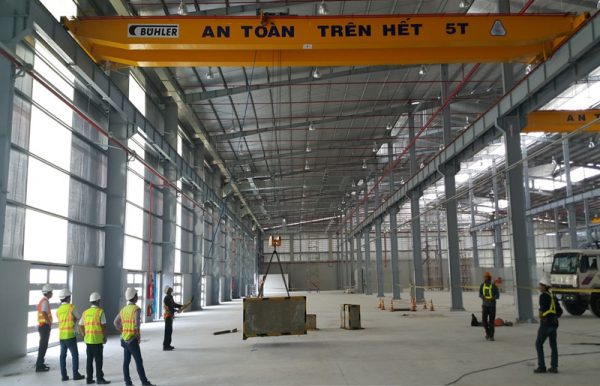
\includegraphics[width=186mm]{../../public/introsection1.jpg}};
  \fill[TTCDeepNavy, opacity=0.84] (0,0) rectangle (74,65);
  \fill[TTCDeepNavy, opacity=0.28] (74,0) rectangle (98,65);
  \node[anchor=west, text width=60mm, align=left, text=white] at (8,43) {
    {\fontsize{7}{8}\selectfont\bfseries\color{TTCCyan} FIELD-BASED LEARNING}\\[1.4mm]
    {\fontsize{15}{17}\selectfont\bfseries 现场即课堂\\实战铸专才}\\[1.8mm]
    {\fontsize{7}{8.6}\selectfont\color{white!82!gray}
    紧扣实际工况与专业设备实操，全员坚决行使安全隐患“一票停工权”。}
  };
  \node[
    anchor=south east, rounded corners=3pt,
    fill=white, fill opacity=0.94, text opacity=1,
    draw=TTCCyan, line width=0.65pt,
    minimum width=52mm, minimum height=13mm, align=center
  ] at (179,7) {
    {\fontsize{8.2}{9.5}\selectfont\bfseries\color{TTCBlue} SAFETY BEFORE PRODUCTIVITY}\\[0.6mm]
    {\fontsize{6.4}{7.8}\selectfont\color{TTCTextDark}安全生产是一切施工作业不可逾越的前提}
  };
  \draw[white, line width=1pt, rounded corners=3pt] (0.6,0.6) rectangle (185.4,64.4);
  \draw[TTCBorder, line width=0.65pt, rounded corners=3pt] (0,0) rectangle (186,65);
\end{tikzpicture}

\vspace{3.5mm}

\noindent
\begin{tikzpicture}[x=1mm,y=1mm]
  \path[use as bounding box] (0,0) rectangle (186,53);
  \node[anchor=west] at (0,48) {
    {\fontsize{7}{8}\selectfont\bfseries\color{TTCCyan} DEVELOPMENT JOURNEY}\quad
    {\fontsize{9.5}{11}\selectfont\bfseries\color{TTCBlue} 从现场工程师到工程领军人才的晋升发展路径}
  };
  \draw[TTCBlue!28!white, line width=0.8pt] (22,30) -- (164,30);

  \foreach \x/\num in {22/01,69/02,117/03,164/04}{
    \fill[white] (\x,30) circle (5);
    \draw[TTCBlue!45!white, line width=0.75pt] (\x,30) circle (5);
    \node[text=TTCBlue, font=\fontsize{7}{8}\selectfont\bfseries] at (\x,30) {\num};
  }
  \fill[TTCRed] (164,30) circle (5);
  \node[text=white, font=\fontsize{7}{8}\selectfont\bfseries] at (164,30) {04};

  \node[align=center, text width=36mm] at (22,13) {
    {\fontsize{8.8}{10}\selectfont\bfseries\color{TTCBlue} HSE READY}\\[0.7mm]
    {\fontsize{6.5}{7.8}\selectfont 100\% 岗前安全三级教育培训}
  };
  \node[align=center, text width=36mm] at (69,13) {
    {\fontsize{8.8}{10}\selectfont\bfseries\color{TTCBlue} TECHNICAL MASTERY}\\[0.7mm]
    {\fontsize{6.5}{7.8}\selectfont BIM • Tekla • MEP • PEB • QA/QC}
  };
  \node[align=center, text width=36mm] at (117,13) {
    {\fontsize{8.8}{10}\selectfont\bfseries\color{TTCBlue} CERTIFIED PRO}\\[0.7mm]
    {\fontsize{6.5}{7.8}\selectfont 建设部二级 • AWS D1.1 • PMP • FIDIC}
  };
  \node[align=center, text width=36mm] at (164,13) {
    {\fontsize{8.8}{10}\selectfont\bfseries\color{TTCRed} PROJECT LEADER}\\[0.7mm]
    {\fontsize{6.5}{7.8}\selectfont 独当一面、引领大型FDI项目总包}
  };
\end{tikzpicture}

\vspace{3.5mm}

\noindent
\begin{tikzpicture}[x=1mm,y=1mm]
  \path[use as bounding box] (0,0) rectangle (186,49);
  \fill[white, rounded corners=4pt] (0,0) rectangle (91,49);
  \draw[TTCBorder, line width=0.65pt, rounded corners=4pt] (0,0) rectangle (91,49);
  \node[anchor=north west, text width=79mm, align=left] at (6,43) {
    {\fontsize{7}{8}\selectfont\bfseries\color{TTCCyan} TTC TECHNICAL ACADEMY}\\[0.8mm]
    {\fontsize{10}{11.5}\selectfont\bfseries\color{TTCBlue} TTC 建筑科技学院}\\[1.5mm]
    {\fontsize{6.8}{8.4}\selectfont\color{TTCTextDark}
    \textcolor{TTCCyan}{\faCheckCircle}\ \textbf{ConTech \& BIM:} Revit, Tekla LOD 400, Navisworks, CDE。\\[0.8mm]
    \textcolor{TTCCyan}{\faCheckCircle}\ \textbf{专项技能：} AWS D1.1、机电消防、高空作业持证培训。\\[0.8mm]
    \textcolor{TTCCyan}{\faCheckCircle}\ \textbf{项目管理：} PMP、FIDIC 合同管理与工程量造价控制。}
  };

  \fill[TTCLightBlue, rounded corners=4pt] (95,0) rectangle (186,49);
  \draw[TTCBorder, line width=0.65pt, rounded corners=4pt] (95,0) rectangle (186,49);
  \node[anchor=north west, text width=79mm, align=left] at (101,43) {
    {\fontsize{7}{8}\selectfont\bfseries\color{TTCRed} SAFETY \& CULTURE SYSTEM}\\[0.8mm]
    {\fontsize{10}{11.5}\selectfont\bfseries\color{TTCBlue} 职业安全与人文关怀体系}\\[1.5mm]
    {\fontsize{6.8}{8.4}\selectfont\color{TTCTextDark}
    \textcolor{TTCRed}{\faCheckCircle}\ 每日工前会 (Toolbox Talk) 与常态化消防救援演练。\\[0.8mm]
    \textcolor{TTCRed}{\faCheckCircle}\ 全员 24/7 意外人身险及定期职业健康体检。\\[0.8mm]
    \textcolor{TTCRed}{\faCheckCircle}\ 透明 KPI 激励体系、清晰晋升通道与停工保护机制。}
  };
\end{tikzpicture}

\vspace{3.5mm}

\noindent
\begin{tikzpicture}[x=1mm,y=1mm]
  \path[use as bounding box] (0,0) rectangle (186,28);
  \fill[white, rounded corners=4pt] (0,0) rectangle (186,28);
  \draw[TTCBorder, line width=0.65pt, rounded corners=4pt] (0,0) rectangle (186,28);
  \foreach \x in {46.5,93,139.5}{
    \draw[TTCBorder, line width=0.5pt] (\x,5) -- (\x,23);
  }
  \node[align=center] at (23.25,14) {
    {\fontsize{13.5}{15}\selectfont\bfseries\color{TTCRed} >120 小时}\\[0.7mm]
    {\fontsize{6.6}{7.8}\selectfont\bfseries 年人均工程师培训时长}
  };
  \node[align=center] at (69.75,14) {
    {\fontsize{13.5}{15}\selectfont\bfseries\color{TTCBlue} 100\%}\\[0.7mm]
    {\fontsize{6.6}{7.8}\selectfont\bfseries 全员持安全卡上岗}
  };
  \node[align=center] at (116.25,14) {
    {\fontsize{13.5}{15}\selectfont\bfseries\color{TTCCyan} 100\%}\\[0.7mm]
    {\fontsize{6.6}{7.8}\selectfont\bfseries 24/7 人身安全保险}
  };
  \node[align=center] at (162.75,14) {
    {\fontsize{13.5}{15}\selectfont\bfseries\color{TTCBlue} ZERO}\\[0.7mm]
    {\fontsize{6.6}{7.8}\selectfont\bfseries 零事故核心文化理念}
  };
\end{tikzpicture}
\end{minipage}
\newpage

% ============================================================
% TRANG 11: PEB SUPPLY & QUALITY GATES
% ============================================================
\pageheaderbar{PEB战略制造网络与品控体系}{第11页}
\pagefooterbar{第11页}

\begin{tikzpicture}[remember picture, overlay]
  \fill[TTCLightBlue]
    ([xshift=118mm,yshift=-24mm]current page.north west) --
    ([xshift=210mm,yshift=-24mm]current page.north west) --
    ([xshift=210mm,yshift=-108mm]current page.north west) --
    ([xshift=162mm,yshift=-79mm]current page.north west) -- cycle;
  \fill[TTCRed!4!white]
    ([xshift=0mm,yshift=-224mm]current page.north west) --
    ([xshift=62mm,yshift=-254mm]current page.north west) --
    ([xshift=0mm,yshift=-274mm]current page.north west) -- cycle;
\end{tikzpicture}

\begin{minipage}[t][246mm]{\textwidth}
\secbrand{TTC 受控 PEB 钢结构制造网络}{Strategic Fabrication Network, Resident QA/QC \& Traceable Quality Gates}

\vspace{1mm}
{\fontsize{15}{17}\selectfont\bfseries\color{TTCBlue}
TTC深化设计 • 战略基地制造 • 常驻QC全过程品控\par}
\vspace{1mm}
{\fontsize{7.5}{9}\selectfont\color{TTCTextMuted}
Flexible fabrication capacity with TTC-controlled engineering, inspection and release authority.\par}
\vspace{3mm}

\noindent
\begin{tikzpicture}[x=1mm,y=1mm]
  \path[use as bounding box] (0,0) rectangle (186,64);
  \clip[rounded corners=3pt] (0,0) rectangle (186,64);
  \node[anchor=center, inner sep=0pt] at (93,32)
    {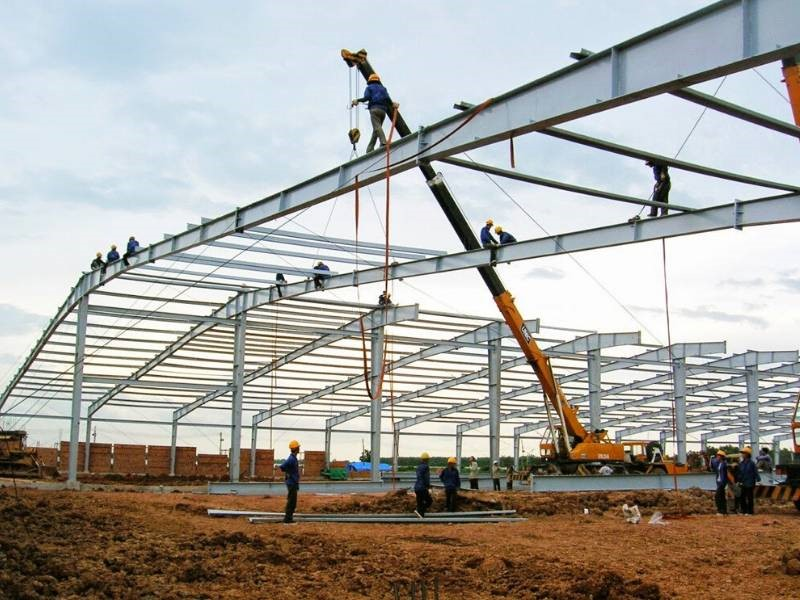
\includegraphics[width=186mm]{../../public/about1.jpg}};
  \fill[TTCDeepNavy, opacity=0.86] (0,0) rectangle (68,64);
  \fill[TTCDeepNavy, opacity=0.28] (68,0) rectangle (92,64);
  \node[anchor=west, text width=54mm, align=left, text=white] at (8,42) {
    {\fontsize{7}{8}\selectfont\bfseries\color{TTCCyan} STRATEGIC PEB NETWORK}\\[1.3mm]
    {\fontsize{19}{21}\selectfont\bfseries 30,000 吨}\\[-0.4mm]
    {\fontsize{8}{9.5}\selectfont\bfseries\color{TTCCyan} 年钢结构供应产能}\\[1.8mm]
    {\fontsize{7}{8.6}\selectfont\color{white!82!gray}
    TTC 全程主导方案设计、加工详图 (Shop Drawing) 及出厂审批。}
  };
  \node[
    anchor=south east, rounded corners=3pt,
    fill=white, fill opacity=0.94, text opacity=1,
    draw=TTCCyan, line width=0.65pt,
    minimum width=55mm, minimum height=14mm, align=center
  ] at (179,7) {
    {\fontsize{9.5}{11}\selectfont\bfseries\color{TTCBlue} >20,000 m\textsuperscript{2} • 常驻 QC 监理}\\[0.6mm]
    {\fontsize{6.5}{7.8}\selectfont\color{TTCTextDark}Partner factory footprint • TTC supervision}
  };
  \draw[white, line width=1pt, rounded corners=3pt] (0.6,0.6) rectangle (185.4,63.4);
  \draw[TTCBorder, line width=0.65pt, rounded corners=3pt] (0,0) rectangle (186,64);
\end{tikzpicture}

\vspace{3mm}

\noindent
\begin{tikzpicture}[x=1mm,y=1mm]
  \path[use as bounding box] (0,0) rectangle (186,53);
  \node[anchor=west] at (0,48) {
    {\fontsize{7}{8}\selectfont\bfseries\color{TTCCyan} FABRICATION FLOW}\quad
    {\fontsize{9.5}{11}\selectfont\bfseries\color{TTCBlue} 六道全闭环精密加工工序}
  };
  \draw[TTCBlue!30!white, line width=0.85pt] (15,31) -- (171,31);

  \foreach \x/\num in {15/01,46/02,77/03,108/04,139/05,171/06}{
    \fill[white] (\x,31) circle (4.8);
    \draw[TTCBlue!48!white, line width=0.75pt] (\x,31) circle (4.8);
    \node[text=TTCBlue, font=\fontsize{6.8}{8}\selectfont\bfseries] at (\x,31) {\num};
  }
  \fill[TTCRed] (171,31) circle (4.8);
  \node[text=white, font=\fontsize{6.8}{8}\selectfont\bfseries] at (171,31) {06};

  \node[align=center, text width=25mm] at (15,13) {
    {\fontsize{8}{9.2}\selectfont\bfseries\color{TTCBlue} CNC 下料}\\[0.6mm]
    {\fontsize{6.3}{7.5}\selectfont 等离子坡口切割}
  };
  \node[align=center, text width=25mm] at (46,13) {
    {\fontsize{8}{9.2}\selectfont\bfseries\color{TTCBlue} 液压组立}\\[0.6mm]
    {\fontsize{6.3}{7.5}\selectfont 自动定位对中}
  };
  \node[align=center, text width=25mm] at (77,13) {
    {\fontsize{8}{9.2}\selectfont\bfseries\color{TTCBlue} 埋弧焊(SAW)}\\[0.6mm]
    {\fontsize{6.3}{7.5}\selectfont AWS D1.1标准}
  };
  \node[align=center, text width=25mm] at (108,13) {
    {\fontsize{8}{9.2}\selectfont\bfseries\color{TTCBlue} 液压矫正}\\[0.6mm]
    {\fontsize{6.3}{7.5}\selectfont 消除焊接热变形}
  };
  \node[align=center, text width=25mm] at (139,13) {
    {\fontsize{8}{9.2}\selectfont\bfseries\color{TTCBlue} 抛丸除锈}\\[0.6mm]
    {\fontsize{6.3}{7.5}\selectfont 达到 Sa 2.5 级}
  };
  \node[align=center, text width=25mm] at (171,13) {
    {\fontsize{8}{9.2}\selectfont\bfseries\color{TTCRed} 涂装防护}\\[0.6mm]
    {\fontsize{6.3}{7.5}\selectfont 环氧与防火涂料}
  };
\end{tikzpicture}

\vspace{3mm}

\noindent
\begin{tikzpicture}[x=1mm,y=1mm]
  \path[use as bounding box] (0,0) rectangle (186,53);

  \fill[white, rounded corners=4pt] (0,0) rectangle (58,53);
  \draw[TTCBorder, line width=0.65pt, rounded corners=4pt] (0,0) rectangle (58,53);
  \node[anchor=north west, text width=48mm, align=left] at (5,47) {
    {\fontsize{7}{8}\selectfont\bfseries\color{TTCCyan} QUALITY GATE 01}\\[0.8mm]
    {\fontsize{10}{11.5}\selectfont\bfseries\color{TTCBlue} 原材料放行关}\\[1.3mm]
    {\fontsize{7}{8.5}\selectfont\color{TTCTextDark}
    \textcolor{TTCCyan}{\faCheckCircle}\ 100\% 钢板 MTC 与质保书追溯。\\[0.7mm]
    \textcolor{TTCCyan}{\faCheckCircle}\ Q345B • SS400 • ASTM A572。\\[0.7mm]
    \textcolor{TTCCyan}{\faCheckCircle}\ 独立第三方力学拉伸与冲击试验。}
  };

  \fill[TTCLightBlue, rounded corners=4pt] (64,0) rectangle (122,53);
  \draw[TTCBlue!50!white, line width=0.7pt, rounded corners=4pt] (64,0) rectangle (122,53);
  \node[anchor=north west, text width=48mm, align=left] at (69,47) {
    {\fontsize{7}{8}\selectfont\bfseries\color{TTCCyan} QUALITY GATE 02}\\[0.8mm]
    {\fontsize{10}{11.5}\selectfont\bfseries\color{TTCBlue} 焊接质量检验关}\\[1.3mm]
    {\fontsize{7}{8.5}\selectfont\color{TTCTextDark}
    \textcolor{TTCBlue}{\faCheckCircle}\ 严格执行核准的 WPS/PQR 规程。\\[0.7mm]
    \textcolor{TTCBlue}{\faCheckCircle}\ 焊工全员持 3G/4G/6G 专业资格证。\\[0.7mm]
    \textcolor{TTCBlue}{\faCheckCircle}\ 关键受力焊缝 100\% UT/MT 超声探伤。}
  };

  \fill[white, rounded corners=4pt] (128,0) rectangle (186,53);
  \draw[TTCRed!65!white, line width=0.75pt, rounded corners=4pt] (128,0) rectangle (186,53);
  \node[anchor=north west, text width=48mm, align=left] at (133,47) {
    {\fontsize{7}{8}\selectfont\bfseries\color{TTCRed} QUALITY GATE 03}\\[0.8mm]
    {\fontsize{10}{11.5}\selectfont\bfseries\color{TTCBlue} 表面涂装与出厂关}\\[1.3mm]
    {\fontsize{7}{8.5}\selectfont\color{TTCTextDark}
    \textcolor{TTCRed}{\faCheckCircle}\ ISO 8501-1 抛丸除锈 Sa 2.5 级。\\[0.7mm]
    \textcolor{TTCRed}{\faCheckCircle}\ Elcometer 数字仪器检测干膜厚度 (DFT)。\\[0.7mm]
    \textcolor{TTCRed}{\faCheckCircle}\ 环氧重防腐与公安消防认证防火涂层。}
  };
\end{tikzpicture}

\vspace{3mm}

\noindent
\begin{tikzpicture}[x=1mm,y=1mm]
  \path[use as bounding box] (0,0) rectangle (186,30);
  \fill[TTCLightBlue, rounded corners=4pt] (0,0) rectangle (186,30);
  \draw[TTCBorder, line width=0.65pt, rounded corners=4pt] (0,0) rectangle (186,30);
  \node[anchor=west, align=left] at (6,15) {
    {\fontsize{7}{8}\selectfont\bfseries\color{TTCCyan} TTC CONTROL MODEL}\\[0.7mm]
    {\fontsize{9.3}{10.8}\selectfont\bfseries\color{TTCBlue} TTC 独家出厂放行权}
  };
  \node[text=TTCRed] at (55,15) {\faChevronRight};
  \node[align=center] at (76,15) {
    {\fontsize{8.5}{10}\selectfont\bfseries\color{TTCBlue} 设计与详图}\\[0.5mm]
    {\fontsize{6.3}{7.5}\selectfont TTC 统一出图}
  };
  \node[text=TTCRed] at (97,15) {\faChevronRight};
  \node[align=center] at (117,15) {
    {\fontsize{8.5}{10}\selectfont\bfseries\color{TTCBlue} 驻厂 QA/QC}\\[0.5mm]
    {\fontsize{6.3}{7.5}\selectfont 全工序旁站监督}
  };
  \node[text=TTCRed] at (138,15) {\faChevronRight};
  \node[align=center] at (162,15) {
    {\fontsize{8.5}{10}\selectfont\bfseries\color{TTCRed} 签发质保放行}\\[0.5mm]
    {\fontsize{6.3}{7.5}\selectfont 无签字严禁发货}
  };
\end{tikzpicture}
\end{minipage}
\newpage

% ============================================================
% TRANG 12: THIẾT BỊ THEO GÓI HUY ĐỘNG
% ============================================================
\pageheaderbar{现场重型机械设备与调度能力}{第12页}
\pagefooterbar{第12页}

\begin{tikzpicture}[remember picture, overlay]
  \fill[TTCLightBlue]
    ([xshift=137mm,yshift=-31mm]current page.north west) --
    ([xshift=210mm,yshift=-31mm]current page.north west) --
    ([xshift=210mm,yshift=-104mm]current page.north west) -- cycle;
  \draw[TTCBlue!8!white, line width=12pt]
    ([xshift=151mm,yshift=42mm]current page.south west) --
    ([xshift=205mm,yshift=96mm]current page.south west);
  \draw[TTCRed!8!white, line width=3pt]
    ([xshift=160mm,yshift=42mm]current page.south west) --
    ([xshift=205mm,yshift=87mm]current page.south west);
  \begin{scope}[shift={(current page.south west)},x=1mm,y=1mm,opacity=.48]
    \draw[TTCBlue!18!white, line width=.7pt] (12,13) -- (198,13);
    \fill[TTCBlue!2!white] (14,13) -- (14,34) -- (34,43) -- (54,34) --
      (54,13) -- cycle;
    \draw[TTCBlue!17!white, line width=.65pt] (14,13) -- (14,34) -- (34,43) --
      (54,34) -- (54,13);
    \foreach \x in {19,27,35,43,51}{\draw[TTCBlue!13!white] (\x,13) -- (\x,34);}
    \fill[TTCBlue!2!white] (61,13) rectangle (133,31);
    \draw[TTCBlue!17!white, line width=.65pt] (61,13) rectangle (133,31);
    \foreach \x in {73,85,97,109,121}{\draw[TTCBlue!12!white] (\x,13) -- (\x,31);}
    \draw[TTCBlue!17!white] (61,22) -- (133,22);
    \draw[TTCBlue!20!white, line width=.85pt] (151,13) -- (151,51);
    \draw[TTCBlue!18!white] (146,13) -- (151,51) -- (156,13);
    \draw[TTCBlue!20!white, line width=.85pt] (151,48) -- (198,48);
    \draw[TTCBlue!17!white] (151,48) -- (177,39) -- (198,48);
    \draw[TTCRed!22!white, line width=.7pt] (184,48) -- (184,25);
    \draw[TTCRed!22!white] (181,25) -- (187,25);
  \end{scope}
\end{tikzpicture}

\begin{minipage}[t][246mm]{\textwidth}
\secbrand{施工机械配置与现场调度保障}{Right Equipment, Right Workfront, Right Time}

{\fontsize{15}{17}\selectfont\bfseries\color{TTCBlue}
43+ 重型机械 • 4 大作业包 • 统筹高效调度\par}
\vspace{1mm}
{\fontsize{7.5}{9}\selectfont\color{TTCTextMuted}
设备按施工关键线路与实战工况精准匹配，全部经法定检测合格，杜绝现场窝工与等待。\par}
\vspace{3mm}

\noindent
\begin{tikzpicture}[x=1mm,y=1mm]
  \path[use as bounding box] (0,0) rectangle (186,58);
  \clip[rounded corners=3pt] (0,0) rectangle (186,58);
  \node[anchor=center, inner sep=0pt] at (93,29)
    {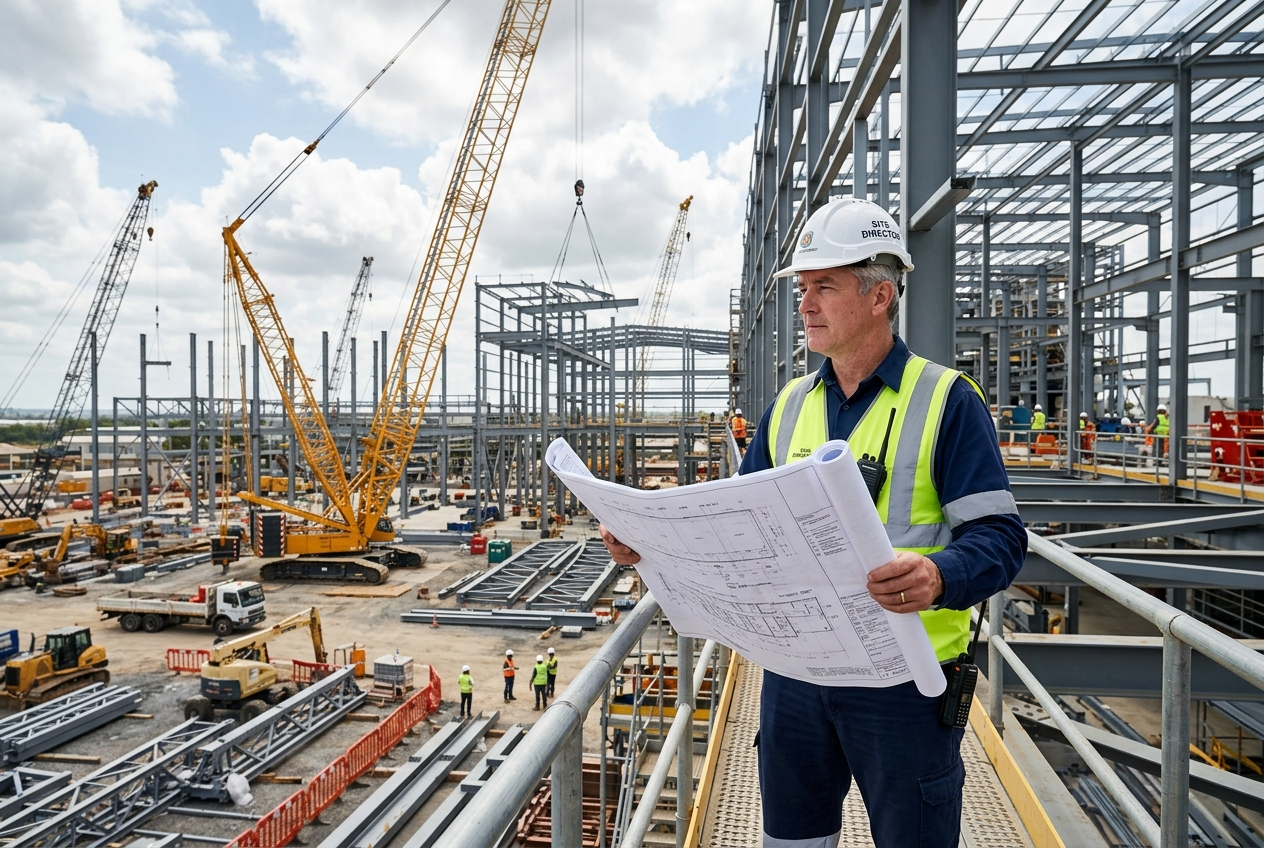
\includegraphics[width=186mm]{../../public/c_level_site_inspection.jpg}};
  \fill[TTCDeepNavy, opacity=0.88] (0,0) rectangle (68,58);
  \fill[TTCDeepNavy, opacity=0.35] (68,0) rectangle (94,58);
  \node[anchor=west, text width=54mm, align=left, text=white] at (8,38) {
    {\fontsize{7}{8}\selectfont\bfseries\color{TTCCyan} MOBILIZATION CONTROL}\\[1.5mm]
    {\fontsize{21}{22}\selectfont\bfseries 43+}\\[-0.5mm]
    {\fontsize{9}{10.5}\selectfont\bfseries 重型施工机械就绪}\\[1.7mm]
    {\fontsize{7}{8.5}\selectfont\color{white!82!gray}
    按项目进度关键线路科学调配，保障施工作业面高效运转。}
  };
  \node[rounded corners=2pt, fill=white, text=TTCBlue, align=center,
        minimum width=31mm, minimum height=16mm] at (129,17) {
    {\fontsize{13}{14}\selectfont\bfseries 100T}\\[-0.4mm]
    {\fontsize{6.2}{7.4}\selectfont 最大汽车吊起重量}
  };
  \node[rounded corners=2pt, fill=TTCRed, text=white, align=center,
        minimum width=35mm, minimum height=16mm] at (167,17) {
    {\fontsize{11}{12}\selectfont\bfseries 100\%}\\[-0.4mm]
    {\fontsize{6.2}{7.4}\selectfont 特种设备年检合格}
  };
\end{tikzpicture}

\vspace{3mm}

\noindent
\begin{tikzpicture}[x=1mm,y=1mm]
  \path[use as bounding box] (0,0) rectangle (186,50);
  \foreach \x/\accent in {0/TTCRed,47.5/TTCCyan,95/TTCBlue,142.5/TTCGold}{
    \fill[white, rounded corners=2pt] (\x,0) rectangle +(43.5,50);
    \draw[TTCBorder, rounded corners=2pt, line width=.55pt] (\x,0) rectangle +(43.5,50);
    \fill[\accent, rounded corners=2pt] (\x,46) rectangle +(43.5,4);
  }
  \node[anchor=north west, text width=35mm, align=left] at (4,43) {
    {\fontsize{15}{16}\selectfont\bfseries\color{TTCRed} 20}\\[-.5mm]
    {\fontsize{7.4}{8.5}\selectfont\bfseries\color{TTCBlue} 起重吊装与高空作业}\\[1mm]
    {\fontsize{6.6}{8}\selectfont\color{TTCTextDark}
    06台 25--100T 汽车吊\newline
    14台 18--28m 高空作业车\newline
    用于钢结构、屋面及机电安装。}
  };
  \node[anchor=north west, text width=35mm, align=left] at (51.5,43) {
    {\fontsize{15}{16}\selectfont\bfseries\color{TTCCyan} 12}\\[-.5mm]
    {\fontsize{7.4}{8.5}\selectfont\bfseries\color{TTCBlue} 地基开挖与混凝土}\\[1mm]
    {\fontsize{6.6}{8}\selectfont\color{TTCTextDark}
    08台 挖掘机与压路机\newline
    04台 泵车与搅拌运输车\newline
    用于基础管网与工业地坪施工。}
  };
  \node[anchor=north west, text width=35mm, align=left] at (99,43) {
    {\fontsize{15}{16}\selectfont\bfseries\color{TTCBlue} 02}\\[-.5mm]
    {\fontsize{7.4}{8.5}\selectfont\bfseries\color{TTCBlue} 现场移动压瓦机组}\\[1mm]
    {\fontsize{6.6}{8}\selectfont\color{TTCTextDark}
    02套 移动式压型成型机\newline
    现场直压 Cliplock/Seamlock\newline
    超长板通长无搭接，杜绝渗水。}
  };
  \node[anchor=north west, text width=35mm, align=left] at (146.5,43) {
    {\fontsize{15}{16}\selectfont\bfseries\color{TTCGold} 09}\\[-.5mm]
    {\fontsize{7.4}{8.5}\selectfont\bfseries\color{TTCBlue} 精密测量与检测仪器}\\[1mm]
    {\fontsize{6.6}{8}\selectfont\color{TTCTextDark}
    09套 徕卡全站仪/3D激光仪\newline
    控制轴线、标高与垂直度\newline
    测量误差目标控制在 2mm 内。}
  };
\end{tikzpicture}

\vspace{3mm}

\noindent
\begin{tikzpicture}[x=1mm,y=1mm]
  \path[use as bounding box] (0,0) rectangle (186,42);
  \fill[TTCLightBlue, rounded corners=3pt] (0,0) rectangle (186,42);
  \draw[TTCBorder, rounded corners=3pt, line width=.6pt] (0,0) rectangle (186,42);
  \node[anchor=west, font=\fontsize{8}{9.5}\selectfont\bfseries, text=TTCBlue] at (7,35)
    {\faClock\quad 紧扣关键线路的设备分步进场节拍};
  \draw[TTCBlue!35!white, line width=1pt] (19,19) -- (167,19);
  \foreach \x/\n/\t/\s in {
    21/01/基础工程/勘察 • 土方开挖 • 混凝土,
    69/02/主体结构/钢柱梁吊装 • 高空拼接,
    117/03/屋面围护/现场压型 • 屋面板 • 装修,
    165/04/调试验收/系统检测 • 试运转 • 交付}{
      \fill[white] (\x,19) circle (4.7);
      \draw[TTCBlue, line width=.8pt] (\x,19) circle (4.7);
      \node[font=\fontsize{6.8}{8}\selectfont\bfseries, text=TTCRed] at (\x,19) {\n};
      \node[anchor=north, align=center, text width=38mm] at (\x,12) {
        {\fontsize{6.8}{8}\selectfont\bfseries\color{TTCBlue} \t}\\[-.3mm]
        {\fontsize{5.8}{7}\selectfont\color{TTCTextMuted} \s}
      };
  }
\end{tikzpicture}

\vspace{3mm}

\noindent
\begin{tikzpicture}[x=1mm,y=1mm]
  \path[use as bounding box] (0,0) rectangle (186,29);
  \fill[TTCDeepNavy, rounded corners=3pt] (0,0) rectangle (186,29);
  \foreach \x in {46.5,93,139.5}{\draw[white!35!gray] (\x,6) -- (\x,23);}
  \node[align=center, text=white] at (23.25,15) {{\fontsize{9}{10}\selectfont\bfseries\color{TTCRed} 12 小时}\\[-.3mm]{\fontsize{6.2}{7.4}\selectfont 紧急调配响应}};
  \node[align=center, text=white] at (69.75,15) {{\fontsize{9}{10}\selectfont\bfseries\color{TTCCyan} 100\% 持证}\\[-.3mm]{\fontsize{6.2}{7.4}\selectfont 特种作业持证上岗}};
  \node[align=center, text=white] at (116.25,15) {{\fontsize{9}{10}\selectfont\bfseries 原厂维保}\\[-.3mm]{\fontsize{6.2}{7.4}\selectfont 定期检修保养}};
  \node[align=center, text=white] at (162.75,15) {{\fontsize{9}{10}\selectfont\bfseries\color{TTCGold} 电子台账}\\[-.3mm]{\fontsize{6.2}{7.4}\selectfont 动态运行监测}};
\end{tikzpicture}
\end{minipage}
\newpage

% ============================================================
% TRANG 13: QUẢN TRỊ DỰ ÁN STAGE-GATE
% ============================================================
\pageheaderbar{FIDIC标准八阶段项目管理流程}{第13页}
\pagefooterbar{第13页}

\begin{tikzpicture}[remember picture, overlay]
  \fill[TTCLightBlue]
    ([xshift=118mm,yshift=-32mm]current page.north west) --
    ([xshift=210mm,yshift=-32mm]current page.north west) --
    ([xshift=210mm,yshift=-118mm]current page.north west) -- cycle;
  \node[opacity=.035, font=\fontsize{62}{64}\selectfont\bfseries, text=TTCBlue,
        rotate=90] at ([xshift=-10mm,yshift=18mm]current page.east) {GATE};
  \begin{scope}[shift={(current page.south west)},x=1mm,y=1mm,opacity=.42]
    \foreach \x/\c in {15/TTCRed,60/TTCCyan,105/TTCBlue,150/TTCGold}{
      \fill[\c!7!white] (\x,14) -- ++(31,0) -- ++(10,14) -- ++(-10,14) --
        ++(-31,0) -- ++(10,-14) -- cycle;
    }
    \node[text=TTCRed!35!white,font=\fontsize{7}{8}\selectfont\bfseries] at (35,28) {DEFINE};
    \node[text=TTCCyan!40!white,font=\fontsize{7}{8}\selectfont\bfseries] at (80,28) {ENGINEER};
    \node[text=TTCBlue!35!white,font=\fontsize{7}{8}\selectfont\bfseries] at (125,28) {BUILD};
    \node[text=TTCGold!40!white,font=\fontsize{7}{8}\selectfont\bfseries] at (170,28) {HANDOVER};
  \end{scope}
\end{tikzpicture}

\begin{minipage}[t][246mm]{\textwidth}
\secbrand{EPC项目 Stage-Gate 四阶段管控体系}{FIDIC Turnkey Governance, Decision Gates \& Single-Point Accountability}

{\fontsize{15}{17}\selectfont\bfseries\color{TTCBlue}
各阶段必有交付成果 • 阶段转换必经核准放行\par}
\vspace{1mm}
{\fontsize{7.5}{9}\selectfont\color{TTCTextMuted}
将八项核心工作整合为四大管控阶段，使业主对决策节点、责任分工及工程状态一目了然。\par}
\vspace{3mm}

\noindent
\begin{tikzpicture}[x=1mm,y=1mm]
  \path[use as bounding box] (0,0) rectangle (186,103);

  % PHASE 01
  \fill[white, rounded corners=2pt] (0,0) rectangle (43.5,103);
  \draw[TTCBorder, rounded corners=2pt, line width=.65pt] (0,0) rectangle (43.5,103);
  \fill[TTCDeepNavy, rounded corners=2pt] (0,84) rectangle (43.5,103);
  \node[anchor=west, text=white] at (4,94) {{\fontsize{7}{8}\selectfont 01}\quad{\fontsize{10}{11}\selectfont\bfseries DEFINE 定义}};
  \node[anchor=north west, text width=35.5mm, align=left] at (4,79) {
    {\fontsize{7}{8.5}\selectfont\bfseries\color{TTCRed} 01 • 勘察与需求确认}\\[.7mm]
    {\fontsize{6.2}{7.5}\selectfont\color{TTCTextDark}地质勘探、3D地形测绘、业主功能需求分析与可行性研究报告。\\[3mm]}
    {\fontsize{7}{8.5}\selectfont\bfseries\color{TTCBlue} 02 • 合规与规划报批}\\[.7mm]
    {\fontsize{6.2}{7.5}\selectfont\color{TTCTextDark}1/500 总平规划、环评(ĐTM)、消防审批、施工许可及设计基准。}
  };
  \fill[TTCRed!8!white] (3.5,5) rectangle (40,17);
  \node[align=center, text=TTCRed] at (21.75,11) {{\fontsize{6}{7}\selectfont\bfseries 关口 A (GATE A)}\\[-.2mm]{\fontsize{5.7}{6.7}\selectfont 基准核准放行}};

  % PHASE 02
  \fill[white, rounded corners=2pt] (47.5,0) rectangle (91,103);
  \draw[TTCBorder, rounded corners=2pt, line width=.65pt] (47.5,0) rectangle (91,103);
  \fill[TTCBlue, rounded corners=2pt] (47.5,84) rectangle (91,103);
  \node[anchor=west, text=white] at (51.5,94) {{\fontsize{7}{8}\selectfont 02}\quad{\fontsize{10}{11}\selectfont\bfseries ENGINEER 深化}};
  \node[anchor=north west, text width=35.5mm, align=left] at (51.5,79) {
    {\fontsize{7}{8.5}\selectfont\bfseries\color{TTCCyan} 03 • 价值工程与BIM}\\[.7mm]
    {\fontsize{6.2}{7.5}\selectfont\color{TTCTextDark}BIM LOD 400 建模、结构截面优化、全专业协同与碰撞检测。\\[3mm]}
    {\fontsize{7}{8.5}\selectfont\bfseries\color{TTCBlue} 04 • 采购与PEB制造}\\[.7mm]
    {\fontsize{6.2}{7.5}\selectfont\color{TTCTextDark}Tier-1材料锁定、加工详图(Shop Drawing)、排产与驻厂QC监督。}
  };
  \fill[TTCCyan!10!white] (51,5) rectangle (87.5,17);
  \node[align=center, text=TTCBlue] at (69.25,11) {{\fontsize{6}{7}\selectfont\bfseries 关口 B (GATE B)}\\[-.2mm]{\fontsize{5.7}{6.7}\selectfont 设计冻结确认}};

  % PHASE 03
  \fill[white, rounded corners=2pt] (95,0) rectangle (138.5,103);
  \draw[TTCBorder, rounded corners=2pt, line width=.65pt] (95,0) rectangle (138.5,103);
  \fill[TTCCyan!85!TTCBlue, rounded corners=2pt] (95,84) rectangle (138.5,103);
  \node[anchor=west, text=white] at (99,94) {{\fontsize{7}{8}\selectfont 03}\quad{\fontsize{10}{11}\selectfont\bfseries BUILD 施工}};
  \node[anchor=north west, text width=35.5mm, align=left] at (99,79) {
    {\fontsize{7}{8.5}\selectfont\bfseries\color{TTCRed} 05 • 地基与园区基建}\\[.7mm]
    {\fontsize{6.2}{7.5}\selectfont\color{TTCTextDark}桩基、承台地梁、工业地坪及室外管网按ITP标准移交作业面。\\[3mm]}
    {\fontsize{7}{8.5}\selectfont\bfseries\color{TTCBlue} 06 • 钢结构与MEP安装}\\[.7mm]
    {\fontsize{6.2}{7.5}\selectfont\color{TTCTextDark}主体钢构吊装、屋面围护、暖通机电、消防及关键线路管控。}
  };
  \fill[TTCBlue!8!white] (98.5,5) rectangle (135,17);
  \node[align=center, text=TTCBlue] at (116.75,11) {{\fontsize{6}{7}\selectfont\bfseries 关口 C (GATE C)}\\[-.2mm]{\fontsize{5.7}{6.7}\selectfont 调试就绪确认}};

  % PHASE 04
  \fill[white, rounded corners=2pt] (142.5,0) rectangle (186,103);
  \draw[TTCBorder, rounded corners=2pt, line width=.65pt] (142.5,0) rectangle (186,103);
  \fill[TTCGold, rounded corners=2pt] (142.5,84) rectangle (186,103);
  \node[anchor=west, text=white] at (146.5,94) {{\fontsize{7}{8}\selectfont 04}\quad{\fontsize{10}{11}\selectfont\bfseries HANDOVER 交付}};
  \node[anchor=north west, text width=35.5mm, align=left] at (146.5,79) {
    {\fontsize{7}{8.5}\selectfont\bfseries\color{TTCRed} 07 • 调试与官方验收}\\[.7mm]
    {\fontsize{6.2}{7.5}\selectfont\color{TTCTextDark}ITP四层验收、消防验收、单机试车及系统联动试运转。\\[3mm]}
    {\fontsize{7}{8.5}\selectfont\bfseries\color{TTCBlue} 08 • 移交与全寿命运维}\\[.7mm]
    {\fontsize{6.2}{7.5}\selectfont\color{TTCTextDark}竣工档案、数字孪生交付、操作人员培训、24个月保修与运维。}
  };
  \fill[TTCGold!12!white] (146,5) rectangle (182.5,17);
  \node[align=center, text=TTCGold!80!black] at (164.25,11) {{\fontsize{6}{7}\selectfont\bfseries 关口 D (GATE D)}\\[-.2mm]{\fontsize{5.7}{6.7}\selectfont 投产运营确认}};

  % Markers
  \foreach \x/\l in {45.5/A,93/B,140.5/C}{
    \fill[white] (\x,51) circle (3.8);
    \draw[TTCRed, line width=.8pt] (\x,51) circle (3.8);
    \node[text=TTCRed, font=\fontsize{5.5}{6}\selectfont\bfseries] at (\x,51) {\l};
  }
\end{tikzpicture}

\vspace{3mm}

\noindent
\begin{tikzpicture}[x=1mm,y=1mm]
  \path[use as bounding box] (0,0) rectangle (186,43);
  \fill[TTCLightBlue, rounded corners=3pt] (0,0) rectangle (186,43);
  \draw[TTCBorder, rounded corners=3pt, line width=.6pt] (0,0) rectangle (186,43);
  \node[anchor=west, text=TTCBlue, font=\fontsize{8}{9.5}\selectfont\bfseries] at (7,35)
    {\faProjectDiagram\quad GOVERNANCE SPINE — 一体化全贯穿管理主线};
  \foreach \x in {46.5,93,139.5}{\draw[TTCBorder] (\x,6) -- (\x,28);}
  \node[align=center, text width=39mm] at (23.25,17) {{\fontsize{7}{8}\selectfont\bfseries\color{TTCRed} 项目总监负责制}\\[-.2mm]{\fontsize{5.8}{7}\selectfont\color{TTCTextMuted}单一接口对最终结果负责}};
  \node[align=center, text width=39mm] at (69.75,17) {{\fontsize{7}{8}\selectfont\bfseries\color{TTCBlue} CPM 关键线路}\\[-.2mm]{\fontsize{5.8}{7}\selectfont\color{TTCTextMuted}周滚动前瞻排程控制}};
  \node[align=center, text width=39mm] at (116.25,17) {{\fontsize{7}{8}\selectfont\bfseries\color{TTCCyan} CDE 协同平台}\\[-.2mm]{\fontsize{5.8}{7}\selectfont\color{TTCTextMuted}图纸、RFI与ITP全程可溯}};
  \node[align=center, text width=39mm] at (162.75,17) {{\fontsize{7}{8}\selectfont\bfseries\color{TTCGold} FIDIC 履约风控}\\[-.2mm]{\fontsize{5.8}{7}\selectfont\color{TTCTextMuted}严控范围、变更与法律风险}};
\end{tikzpicture}

\vspace{3mm}

\noindent
\begin{tikzpicture}[x=1mm,y=1mm]
  \path[use as bounding box] (0,0) rectangle (186,29);
  \fill[TTCDeepNavy, rounded corners=3pt] (0,0) rectangle (186,29);
  \foreach \x in {46.5,93,139.5}{\draw[white!35!gray] (\x,6) -- (\x,23);}
  \node[align=center, text=white] at (23.25,15) {{\fontsize{9}{10}\selectfont\bfseries\color{TTCRed} 8 个步骤}\\[-.3mm]{\fontsize{6.2}{7.4}\selectfont 整合为4大管控阶段}};
  \node[align=center, text=white] at (69.75,15) {{\fontsize{9}{10}\selectfont\bfseries\color{TTCCyan} 4 个关口}\\[-.3mm]{\fontsize{6.2}{7.4}\selectfont 严苛条件放行}};
  \node[align=center, text=white] at (116.25,15) {{\fontsize{9}{10}\selectfont\bfseries FIDIC EPC}\\[-.3mm]{\fontsize{6.2}{7.4}\selectfont 国际通用合同标准}};
  \node[align=center, text=white] at (162.75,15) {{\fontsize{9}{10}\selectfont\bfseries\color{TTCGold} 24 个月}\\[-.3mm]{\fontsize{6.2}{7.4}\selectfont 结构全面品质保修}};
\end{tikzpicture}
\end{minipage}
\newpage

% ============================================================
% TRANG 14: EPC VALUE MODEL — ONE CONTRACT, ONE ACCOUNTABILITY
% ============================================================
\pageheaderbar{EPC总承包模式与价值工程}{第14页}
\pagefooterbar{第14页}

\begin{tikzpicture}[remember picture, overlay]
  \fill[TTCLightBlue]
    ([xshift=132mm,yshift=-30mm]current page.north west) --
    ([xshift=210mm,yshift=-30mm]current page.north west) --
    ([xshift=210mm,yshift=-104mm]current page.north west) -- cycle;
  \draw[TTCBlue!7!white, line width=12pt]
    ([xshift=154mm,yshift=37mm]current page.south west) --
    ([xshift=205mm,yshift=88mm]current page.south west);
  \draw[TTCRed!8!white, line width=3pt]
    ([xshift=162mm,yshift=37mm]current page.south west) --
    ([xshift=205mm,yshift=80mm]current page.south west);
  \begin{scope}[shift={(current page.south west)},x=1mm,y=1mm,opacity=.42]
    \draw[TTCBlue!17!white, line width=.7pt] (12,13) -- (198,13);
    \draw[TTCBlue!16!white] (17,13) -- (17,37) -- (47,50) -- (77,37) --
      (107,50) -- (137,37) -- (167,50) -- (197,37) -- (197,13);
    \foreach \x in {17,47,77,107,137,167,197}{\draw[TTCBlue!12!white] (\x,13) -- (\x,42);}
    \draw[TTCRed!18!white, line width=.7pt] (17,20) -- (197,20);
  \end{scope}
\end{tikzpicture}

\begin{minipage}[t][246mm]{\textwidth}
\secbrand{EPC总承包模式与价值工程}{Fast-Track Delivery, Value Engineering \& Single-Point Accountability}

{\fontsize{15}{17}\selectfont\bfseries\color{TTCBlue}
工期更短 • 流程更精简 • 投资风险更低\par}
\vspace{1mm}
{\fontsize{7.5}{9}\selectfont\color{TTCTextMuted}
TTC将法定报批、工程设计、材料采购与施工安装整合于一份总包合同，全流程聚焦业主投资效益。\par}
\vspace{3mm}

\noindent
\begin{tikzpicture}[x=1mm,y=1mm]
  \path[use as bounding box] (0,0) rectangle (186,66);
  \clip[rounded corners=3pt] (0,0) rectangle (186,66);
  \node[anchor=center, inner sep=0pt] at (93,33)
    {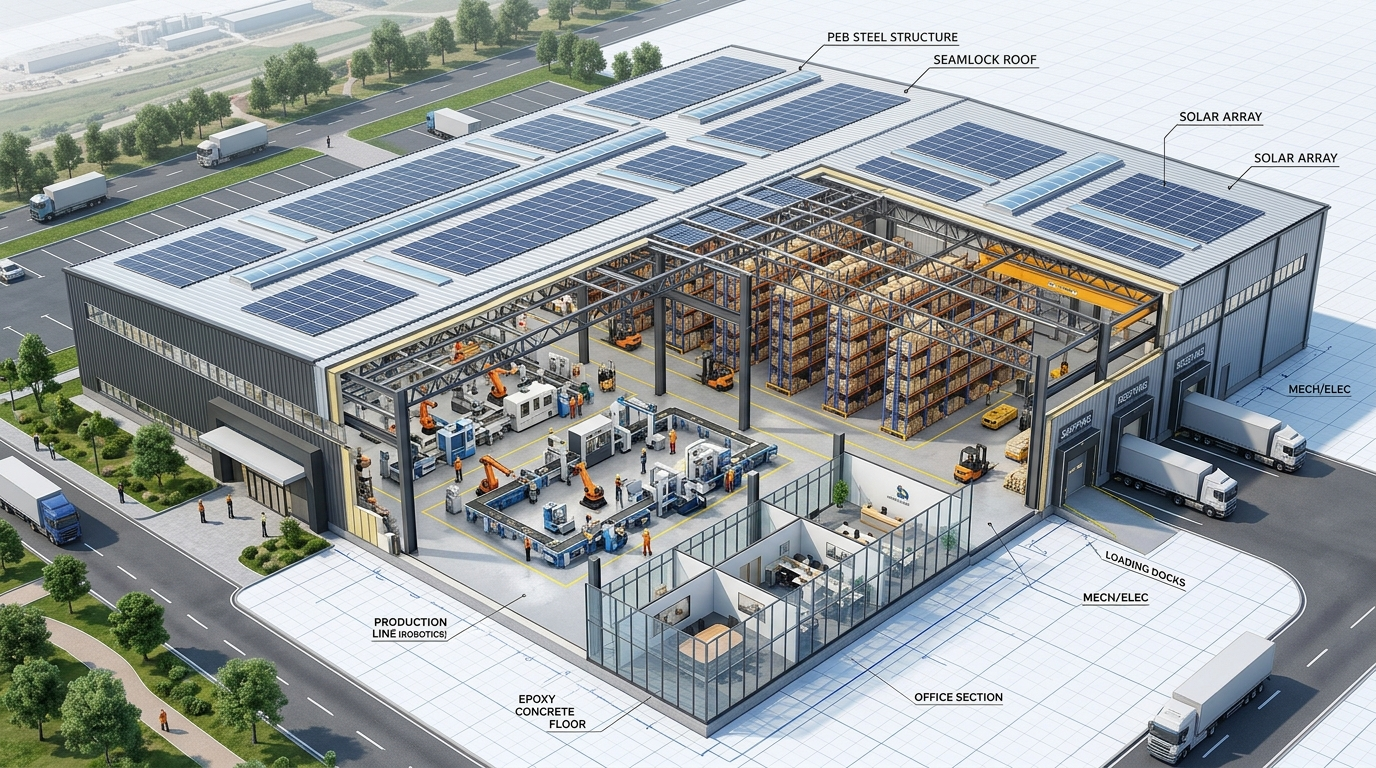
\includegraphics[width=186mm]{../../public/factory-tech-3d.jpg}};
  \fill[TTCDeepNavy, opacity=.88] (0,0) rectangle (66,66);
  \fill[TTCDeepNavy, opacity=.26] (66,0) rectangle (92,66);
  \node[anchor=west, text width=52mm, align=left, text=white] at (8,43) {
    {\fontsize{7}{8}\selectfont\bfseries\color{TTCCyan} TTC EPC VALUE MODEL}\\[1.3mm]
    {\fontsize{17}{19}\selectfont\bfseries ONE CONTRACT}\\[-.2mm]
    {\fontsize{10}{12}\selectfont\bfseries\color{TTCRed!85!white} ONE ACCOUNTABILITY}\\[1.7mm]
    {\fontsize{7}{8.5}\selectfont\color{white!82!gray}
    单一总包主体严密管控工程范围、投资预算、施工进度与交付质量。}
  };
  \node[rounded corners=2pt, fill=white, align=center, minimum width=29mm,
        minimum height=15mm] at (113,15) {
    {\fontsize{11}{12}\selectfont\bfseries\color{TTCRed} -15\%}\\[-.3mm]
    {\fontsize{5.8}{7}\selectfont\color{TTCBlue} 优化用钢量}
  };
  \node[rounded corners=2pt, fill=white, align=center, minimum width=29mm,
        minimum height=15mm] at (145,15) {
    {\fontsize{11}{12}\selectfont\bfseries\color{TTCCyan} -60 天}\\[-.3mm]
    {\fontsize{5.8}{7}\selectfont\color{TTCBlue} 缩短项目工期}
  };
  \node[rounded corners=2pt, fill=TTCGold, text=white, align=center,
        minimum width=29mm, minimum height=15mm] at (177,15) {
    {\fontsize{11}{12}\selectfont\bfseries 0}\\[-.3mm]
    {\fontsize{5.8}{7}\selectfont MEP机电碰撞}
  };
\end{tikzpicture}

\vspace{3mm}

\noindent
\begin{tikzpicture}[x=1mm,y=1mm]
  \path[use as bounding box] (0,0) rectangle (186,48);
  \fill[TTCLightBlue, rounded corners=3pt] (0,0) rectangle (186,48);
  \draw[TTCBorder, rounded corners=3pt, line width=.6pt] (0,0) rectangle (186,48);
  \node[anchor=west, text=TTCBlue, font=\fontsize{8}{9.5}\selectfont\bfseries] at (7,40)
    {\faProjectDiagram\quad 六大业务工作流 — 一体化价值链};
  \draw[TTCBlue!35!white, line width=1pt] (14,23) -- (172,23);
  \foreach \x/\n/\t/\s in {
    16/01/DEFINE/报批与需求,
    47/02/OPTIMIZE/VE与BIM 5D,
    78/03/ENGINEER/加工详图深化,
    109/04/FABRICATE/PEB制造供应,
    140/05/BUILD/基础与机电,
    171/06/OPERATE/数字孪生运维}{
      \fill[white] (\x,23) circle (4.6);
      \draw[TTCBlue, line width=.75pt] (\x,23) circle (4.6);
      \node[text=TTCRed,font=\fontsize{6.4}{7}\selectfont\bfseries] at (\x,23) {\n};
      \node[anchor=north,align=center,text width=27mm] at (\x,16) {
        {\fontsize{6.6}{7.8}\selectfont\bfseries\color{TTCBlue} \t}\\[-.2mm]
        {\fontsize{5.7}{6.8}\selectfont\color{TTCTextMuted} \s}
      };
  }
\end{tikzpicture}

\vspace{3mm}

\noindent
\begin{tikzpicture}[x=1mm,y=1mm]
  \path[use as bounding box] (0,0) rectangle (186,49);
  \foreach \x/\c in {0/TTCRed,63/TTCCyan,126/TTCGold}{
    \fill[white, rounded corners=2pt] (\x,0) rectangle +(60,49);
    \draw[TTCBorder, rounded corners=2pt, line width=.6pt] (\x,0) rectangle +(60,49);
    \fill[\c, rounded corners=2pt] (\x,45) rectangle +(60,4);
  }
  \node[anchor=north west, text width=50mm] at (5,40) {
    {\fontsize{8}{9.5}\selectfont\bfseries\color{TTCRed} 01 • 精益设计}\\[1mm]
    {\fontsize{10}{11}\selectfont\bfseries\color{TTCBlue} 结构截面优化}\\[1mm]
    {\fontsize{6.8}{8.2}\selectfont\color{TTCTextDark}
    按受力包络线采用变截面门架，减轻基础荷载同时确保安全储备。}
  };
  \node[anchor=north west, text width=50mm] at (68,40) {
    {\fontsize{8}{9.5}\selectfont\bfseries\color{TTCCyan} 02 • 提前穿插}\\[1mm]
    {\fontsize{10}{11}\selectfont\bfseries\color{TTCBlue} 并行交叉推进}\\[1mm]
    {\fontsize{6.8}{8.2}\selectfont\color{TTCTextDark}
    方案设计、PEB构件排产与现场桩基土建按关键线路并行实施。}
  };
  \node[anchor=north west, text width=50mm] at (131,40) {
    {\fontsize{8}{9.5}\selectfont\bfseries\color{TTCGold} 03 • 锁定风控}\\[1mm]
    {\fontsize{10}{11}\selectfont\bfseries\color{TTCBlue} 严控变更与造价}\\[1mm]
    {\fontsize{6.8}{8.2}\selectfont\color{TTCTextDark}
    BIM碰撞检测、出厂关口放行与总价包干合同有效杜绝额外签证。}
  };
\end{tikzpicture}

\vspace{3mm}

\noindent
\begin{tikzpicture}[x=1mm,y=1mm]
  \path[use as bounding box] (0,0) rectangle (186,29);
  \fill[TTCDeepNavy, rounded corners=3pt] (0,0) rectangle (186,29);
  \foreach \x in {46.5,93,139.5}{\draw[white!35!gray] (\x,6) -- (\x,23);}
  \node[align=center,text=white] at (23.25,15) {{\fontsize{9}{10}\selectfont\bfseries\color{TTCRed} 成本优化}\\[-.3mm]{\fontsize{6.2}{7.4}\selectfont 价值工程 (VE)}};
  \node[align=center,text=white] at (69.75,15) {{\fontsize{9}{10}\selectfont\bfseries\color{TTCCyan} 45--60 天}\\[-.3mm]{\fontsize{6.2}{7.4}\selectfont Fast-Track 快速建造}};
  \node[align=center,text=white] at (116.25,15) {{\fontsize{9}{10}\selectfont\bfseries 0 碰撞}\\[-.3mm]{\fontsize{6.2}{7.4}\selectfont BIM 全专业协同}};
  \node[align=center,text=white] at (162.75,15) {{\fontsize{9}{10}\selectfont\bfseries\color{TTCGold} 总价包干}\\[-.3mm]{\fontsize{6.2}{7.4}\selectfont 预算确定性保障}};
\end{tikzpicture}
\end{minipage}
\newpage

% ============================================================
% TRANG 15: DIGITAL THREAD — BIM, AI, DIGITAL TWIN
% ============================================================
\pageheaderbar{建筑科技：BIM 5D、AI与智能数字孪生}{第15页}
\pagefooterbar{第15页}

\begin{tikzpicture}[remember picture, overlay]
  \fill[TTCLightBlue]
    ([xshift=122mm,yshift=-31mm]current page.north west) --
    ([xshift=210mm,yshift=-31mm]current page.north west) --
    ([xshift=210mm,yshift=-111mm]current page.north west) -- cycle;
  \node[opacity=.03, text=TTCBlue, font=\fontsize{62}{64}\selectfont\bfseries,
        rotate=90] at ([xshift=-11mm,yshift=7mm]current page.east) {DATA};
  \begin{scope}[shift={(current page.south west)},x=1mm,y=1mm,opacity=.40]
    \draw[TTCBlue!17!white, line width=.8pt] (14,15) -- (196,15);
    \foreach \x in {22,58,94,130,166}{
      \draw[TTCBlue!15!white] (\x,15) -- (\x+12,36) -- (\x+24,15);
      \fill[TTCCyan!10!white] (\x+12,36) circle (2.2);
    }
    \draw[TTCRed!18!white, line width=.7pt] (22,23) -- (190,23);
  \end{scope}
\end{tikzpicture}

\begin{minipage}[t][246mm]{\textwidth}
\secbrand{贯穿工厂全生命周期的数字孪生数据流}{BIM 5D, AI Structural Optimization \& Smart Digital Twin}

{\fontsize{15}{17}\selectfont\bfseries\color{TTCBlue}
统一数据模型 • 三维智能决策 • 赋能全生命周期\par}
\vspace{1mm}
{\fontsize{7.5}{9}\selectfont\color{TTCTextMuted}
设计数据不再停留在图纸上：它直接指导采购制造、现场施工、竣工验收以及长达30+年的智慧运维。\par}
\vspace{3mm}

\noindent
\begin{tikzpicture}[x=1mm,y=1mm]
  \path[use as bounding box] (0,0) rectangle (186,68);
  \clip[rounded corners=3pt] (0,0) rectangle (186,68);
  \node[anchor=center,inner sep=0pt] at (93,34)
    {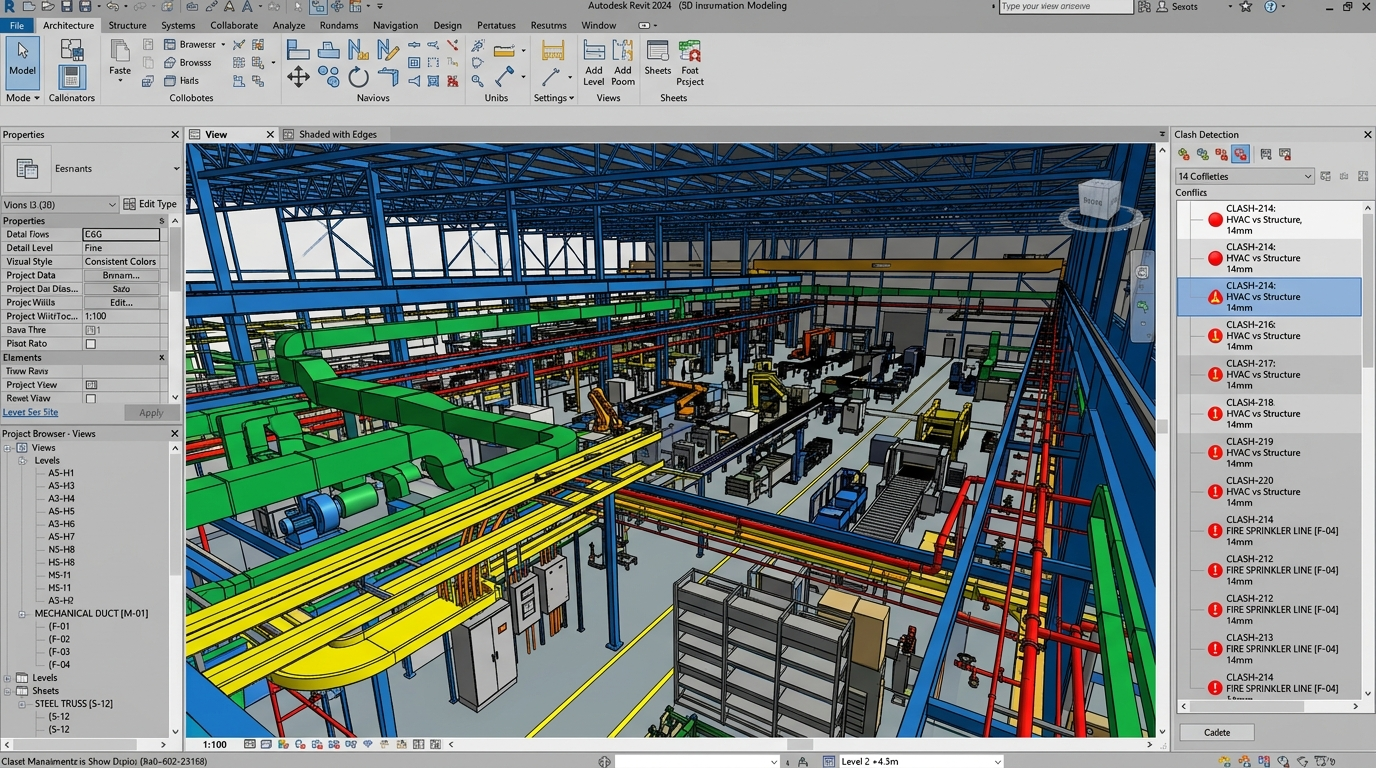
\includegraphics[width=186mm]{../../public/bim-model-3d.jpg}};
  \fill[TTCDeepNavy,opacity=.88] (0,0) rectangle (61,68);
  \fill[TTCDeepNavy,opacity=.24] (61,0) rectangle (86,68);
  \node[anchor=west,text width=48mm,align=left,text=white] at (8,44) {
    {\fontsize{7}{8}\selectfont\bfseries\color{TTCCyan} TTC DIGITAL THREAD}\\[1.4mm]
    {\fontsize{17}{19}\selectfont\bfseries 数据驱动}\\[-.3mm]
    {\fontsize{17}{19}\selectfont\bfseries\color{TTCRed!85!white} 科学决策}\\[1.8mm]
    {\fontsize{7}{8.5}\selectfont\color{white!82!gray}
    为设计院、施工指挥部与业主运营团队提供唯一可信数据源。}
  };
  \node[rounded corners=2pt,fill=white,align=center,minimum width=27mm,
        minimum height=15mm] at (111,15) {
    {\fontsize{9}{10}\selectfont\bfseries\color{TTCBlue} DESIGN}\\[-.2mm]
    {\fontsize{5.8}{7}\selectfont LOD 400 • 5D}
  };
  \node[rounded corners=2pt,fill=TTCCyan,align=center,text=white,
        minimum width=27mm,minimum height=15mm] at (143,15) {
    {\fontsize{9}{10}\selectfont\bfseries BUILD}\\[-.2mm]
    {\fontsize{5.8}{7}\selectfont Clash • 4D}
  };
  \node[rounded corners=2pt,fill=TTCGold,align=center,text=white,
        minimum width=27mm,minimum height=15mm] at (172,15) {
    {\fontsize{9}{10}\selectfont\bfseries OPERATE}\\[-.2mm]
    {\fontsize{5.8}{7}\selectfont Twin • O\&M}
  };
\end{tikzpicture}

\vspace{3mm}

\noindent
\begin{tikzpicture}[x=1mm,y=1mm]
  \path[use as bounding box] (0,0) rectangle (186,62);
  \foreach \x/\c in {0/TTCRed,63/TTCCyan,126/TTCGold}{
    \fill[white,rounded corners=2pt] (\x,0) rectangle +(60,62);
    \draw[TTCBorder,rounded corners=2pt,line width=.6pt] (\x,0) rectangle +(60,62);
    \fill[\c,rounded corners=2pt] (\x,58) rectangle +(60,4);
  }
  \node[anchor=north west,text width=50mm] at (5,53) {
    {\fontsize{7}{8}\selectfont\bfseries\color{TTCRed} 01 / 协同深化}\\[1mm]
    {\fontsize{11}{12}\selectfont\bfseries\color{TTCBlue} BIM 5D 全专业}\\[1.2mm]
    {\fontsize{6.8}{8.2}\selectfont\color{TTCTextDark}
    \textbf{输入：} 建筑 • 结构 • 机电MEP\newline
    \textbf{决策：} 碰撞检测与4D施工模拟\newline
    \textbf{输出：} 加工详图、精确BOQ清单}\\[1mm]
    {\fontsize{6.2}{7.3}\selectfont\bfseries\color{TTCTextMuted} TEKLA • REVIT • NAVISWORKS}
  };
  \node[anchor=north west,text width=50mm] at (68,53) {
    {\fontsize{7}{8}\selectfont\bfseries\color{TTCCyan} 02 / 智能优化}\\[1mm]
    {\fontsize{11}{12}\selectfont\bfseries\color{TTCBlue} AI 结构计算}\\[1.2mm]
    {\fontsize{6.8}{8.2}\selectfont\color{TTCTextDark}
    \textbf{输入：} 荷载 • 柱网跨度 • 内力包络\newline
    \textbf{决策：} 遗传算法多变量截面迭代\newline
    \textbf{输出：} 结构成本优化 10--15\% 最优方案}\\[1mm]
    {\fontsize{6.2}{7.3}\selectfont\bfseries\color{TTCTextMuted} AISC 360 • EUROCODE • AIDC R\&D}
  };
  \node[anchor=north west,text width=50mm] at (131,53) {
    {\fontsize{7}{8}\selectfont\bfseries\color{TTCGold} 03 / 智慧运营}\\[1mm]
    {\fontsize{11}{12}\selectfont\bfseries\color{TTCBlue} 数字孪生资产}\\[1.2mm]
    {\fontsize{6.8}{8.2}\selectfont\color{TTCTextDark}
    \textbf{输入：} 竣工模型 • 设备台账 • IoT传感\newline
    \textbf{决策：} 基于设备状态的预测性维保\newline
    \textbf{输出：} 30+年可追溯资产数字档案}\\[1mm]
    {\fontsize{6.2}{7.3}\selectfont\bfseries\color{TTCTextMuted} CDE • BMS • SCADA READY}
  };
\end{tikzpicture}
\end{minipage}
\newpage

% ============================================================
% TRANG 16: ESG BUSINESS CASE — GREEN FACTORY
% ============================================================
\pageheaderbar{绿色ESG建筑与屋顶光伏就绪}{第16页}
\pagefooterbar{第16页}

\begin{tikzpicture}[remember picture, overlay]
  \fill[TTCLightBlue]
    ([xshift=125mm,yshift=-30mm]current page.north west) --
    ([xshift=210mm,yshift=-30mm]current page.north west) --
    ([xshift=210mm,yshift=-112mm]current page.north west) -- cycle;
  \node[opacity=.03,text=TTCBlue,font=\fontsize{64}{66}\selectfont\bfseries,
        rotate=90] at ([xshift=-11mm,yshift=2mm]current page.east) {ESG};
  \begin{scope}[shift={(current page.south west)},x=1mm,y=1mm,opacity=.43]
    \draw[TTCBlue!17!white,line width=.7pt] (14,13) -- (196,13);
    \foreach \x in {18,48,78,108,138,168}{
      \fill[TTCBlue!3!white] (\x,14) -- ++(24,0) -- ++(-5,17) -- ++(-24,0) -- cycle;
      \draw[TTCBlue!16!white] (\x,14) -- ++(24,0) -- ++(-5,17) -- ++(-24,0) -- cycle;
      \draw[TTCBlue!11!white] (\x+4,14) -- (\x-1,31);
      \draw[TTCBlue!11!white] (\x+12,14) -- (\x+7,31);
    }
    \draw[TTCCyan!22!white,line width=.8pt] (24,38) arc[start angle=210,end angle=330,radius=10mm];
    \draw[TTCRed!18!white,line width=.7pt] (24,38) -- (24,45);
  \end{scope}
\end{tikzpicture}

\begin{minipage}[t][246mm]{\textwidth}
\secbrand{将绿色低碳理念融入工程商业价值模型}{Solar-Ready, Low-Energy Envelope, Water Circularity \& Green Certification}

{\fontsize{15}{17}\selectfont\bfseries\color{TTCBlue}
削减OPEX运营成本 • 顺应碳关税合规 • 提升资产价值\par}
\vspace{1mm}
{\fontsize{7.5}{9}\selectfont\color{TTCTextMuted}
绿色ESG设计从前期结构载荷与围护系统深度集成，避免投产后再行改造带来的高昂成本。\par}
\vspace{3mm}

\noindent
\begin{tikzpicture}[x=1mm,y=1mm]
  \path[use as bounding box] (0,0) rectangle (186,70);
  \clip[rounded corners=3pt] (0,0) rectangle (186,70);
  \node[anchor=center,inner sep=0pt] at (93,35)
    {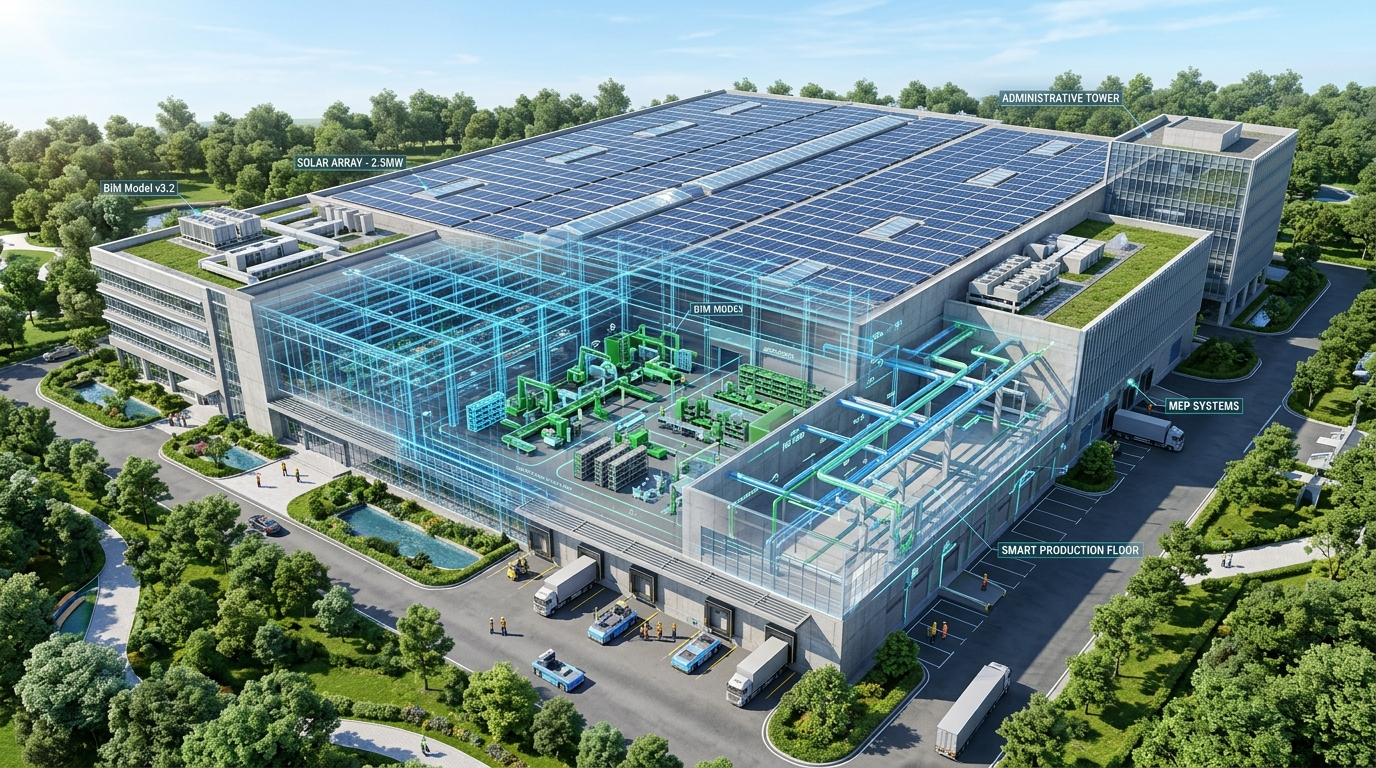
\includegraphics[width=186mm]{../../public/bim-esg-factory-3d.jpg}};
  \fill[TTCDeepNavy,opacity=.84] (0,0) rectangle (61,70);
  \fill[TTCDeepNavy,opacity=.22] (61,0) rectangle (87,70);
  \node[anchor=west,text width=48mm,align=left,text=white] at (8,46) {
    {\fontsize{7}{8}\selectfont\bfseries\color{TTCCyan} ESG-BY-DESIGN}\\[1.3mm]
    {\fontsize{17}{19}\selectfont\bfseries NET-ZERO}\\[-.2mm]
    {\fontsize{17}{19}\selectfont\bfseries\color{TTCRed!85!white} READY}\\[1.8mm]
    {\fontsize{7}{8.5}\selectfont\color{white!82!gray}
    屋顶荷载、能耗模拟、水资源循环与绿色认证协同设计。}
  };
  \node[rounded corners=2pt,fill=white,align=center,minimum width=31mm,
        minimum height=15mm] at (121,15) {
    {\fontsize{10}{11}\selectfont\bfseries\color{TTCRed} 1--5 MWp}\\[-.2mm]
    {\fontsize{5.8}{7}\selectfont\color{TTCBlue} 光伏就绪屋面}
  };
  \node[rounded corners=2pt,fill=TTCCyan,align=center,text=white,
        minimum width=31mm,minimum height=15mm] at (155,15) {
    {\fontsize{10}{11}\selectfont\bfseries -20\%}\\[-.2mm]
    {\fontsize{5.8}{7}\selectfont 暖通能耗降低}
  };
\end{tikzpicture}

\vspace{3mm}

\noindent
\begin{tikzpicture}[x=1mm,y=1mm]
  \path[use as bounding box] (0,0) rectangle (186,51);
  \foreach \x/\c in {0/TTCRed,47.5/TTCCyan,95/TTCBlue,142.5/TTCGold}{
    \fill[white,rounded corners=2pt] (\x,0) rectangle +(43.5,51);
    \draw[TTCBorder,rounded corners=2pt,line width=.6pt] (\x,0) rectangle +(43.5,51);
    \fill[\c,rounded corners=2pt] (\x,47) rectangle +(43.5,4);
  }
  \node[anchor=north west,text width=35mm] at (4,43) {
    {\fontsize{7}{8}\selectfont\bfseries\color{TTCRed} 01 / 清洁能源}\\[1mm]
    {\fontsize{8.5}{10}\selectfont\bfseries\color{TTCBlue} 光伏系统就绪}\\[1mm]
    {\fontsize{6.5}{7.8}\selectfont\color{TTCTextDark}
    预留屋顶荷载与直锁式立缝咬合件，可即装 1--5MWp 光伏。}
  };
  \node[anchor=north west,text width=35mm] at (51.5,43) {
    {\fontsize{7}{8}\selectfont\bfseries\color{TTCCyan} 02 / 节能围护}\\[1mm]
    {\fontsize{8.5}{10}\selectfont\bfseries\color{TTCBlue} 高效隔热系统}\\[1mm]
    {\fontsize{6.5}{7.8}\selectfont\color{TTCTextDark}
    PIR/岩棉夹芯板与高反射涂层屋面大幅降低暖通空调能耗。}
  };
  \node[anchor=north west,text width=35mm] at (99,43) {
    {\fontsize{7}{8}\selectfont\bfseries\color{TTCBlue} 03 / 水循环}\\[1mm]
    {\fontsize{8.5}{10}\selectfont\bfseries\color{TTCBlue} 循环回用系统}\\[1mm]
    {\fontsize{6.5}{7.8}\selectfont\color{TTCTextDark}
    QCVN 40 A级污水处理站与雨水收集回用系统用于绿化灌溉。}
  };
  \node[anchor=north west,text width=35mm] at (146.5,43) {
    {\fontsize{7}{8}\selectfont\bfseries\color{TTCGold} 04 / 绿色认证}\\[1mm]
    {\fontsize{8.5}{10}\selectfont\bfseries\color{TTCBlue} LEED / LOTUS}\\[1mm]
    {\fontsize{6.5}{7.8}\selectfont\color{TTCTextDark}
    能耗模拟分析、Low-VOC低挥发材料及全套绿色认证申报支持。}
  };
\end{tikzpicture}

\vspace{3mm}

\noindent
\begin{tikzpicture}[x=1mm,y=1mm]
  \path[use as bounding box] (0,0) rectangle (186,47);
  \fill[TTCLightBlue,rounded corners=3pt] (0,0) rectangle (186,47);
  \draw[TTCBorder,rounded corners=3pt,line width=.6pt] (0,0) rectangle (186,47);
  \node[anchor=west,text=TTCBlue,font=\fontsize{8}{9.5}\selectfont\bfseries] at (7,39)
    {\faGlobeAmericas\quad 赋能外资跨国企业 (FDI) 核心诉求};
  \foreach \x in {62,124}{\draw[TTCBorder] (\x,6) -- (\x,31);}
  \node[align=left,text width=50mm,anchor=north west] at (6,30) {
    {\fontsize{8}{9.5}\selectfont\bfseries\color{TTCRed} 绿色金融准入}\\[.7mm]
    {\fontsize{6.5}{7.8}\selectfont\color{TTCTextDark}
    助力企业轻松对接绿色低息信贷与跨国供应链ESG评级准入标准。}
  };
  \node[align=left,text width=50mm,anchor=north west] at (68,30) {
    {\fontsize{8}{9.5}\selectfont\bfseries\color{TTCCyan} 应对碳关税壁垒}\\[.7mm]
    {\fontsize{6.5}{7.8}\selectfont\color{TTCTextDark}
    精准采集能耗数据，满足欧盟CBAM碳关税、I-REC绿证与零碳路线图。}
  };
  \node[align=left,text width=50mm,anchor=north west] at (130,30) {
    {\fontsize{8}{9.5}\selectfont\bfseries\color{TTCGold} 显著降低OPEX}\\[.7mm]
    {\fontsize{6.5}{7.8}\selectfont\color{TTCTextDark}
    自发自用降低电费支出，优化中水利用，长效提升工厂资产残值。}
  };
\end{tikzpicture}

\vspace{3mm}

\noindent
\begin{tikzpicture}[x=1mm,y=1mm]
  \path[use as bounding box] (0,0) rectangle (186,29);
  \fill[TTCDeepNavy, rounded corners=3pt] (0,0) rectangle (186,29);
  \foreach \x in {46.5,93,139.5}{\draw[white!35!gray] (\x,6) -- (\x,23);}
  \node[align=center,text=white] at (23.25,15) {{\fontsize{9}{10}\selectfont\bfseries\color{TTCRed} 1--5 MWp}\\[-.3mm]{\fontsize{6.2}{7.4}\selectfont 光伏就绪屋顶}};
  \node[align=center,text=white] at (69.75,15) {{\fontsize{9}{10}\selectfont\bfseries\color{TTCCyan} -20\% 电耗}\\[-.3mm]{\fontsize{6.2}{7.4}\selectfont 暖通节能优化}};
  \node[align=center,text=white] at (116.25,15) {{\fontsize{9}{10}\selectfont\bfseries LEED / LOTUS}\\[-.3mm]{\fontsize{6.2}{7.4}\selectfont 国际绿色建筑标准}};
  \node[align=center,text=white] at (162.75,15) {{\fontsize{9}{10}\selectfont\bfseries\color{TTCGold} 100\% A级水}\\[-.3mm]{\fontsize{6.2}{7.4}\selectfont 污水达标循环利用}};
\end{tikzpicture}
\end{minipage}
\newpage

% ============================================================
% TRANG 17: DIGITAL SITE CONTROL CENTER
% ============================================================
\pageheaderbar{数字化智慧工地与AI智能监控}{第17页}
\pagefooterbar{第17页}

\begin{tikzpicture}[remember picture, overlay]
  \fill[TTCLightBlue]
    ([xshift=131mm,yshift=-30mm]current page.north west) --
    ([xshift=210mm,yshift=-30mm]current page.north west) --
    ([xshift=210mm,yshift=-115mm]current page.north west) -- cycle;
  \begin{scope}[shift={(current page.south west)},x=1mm,y=1mm,opacity=.45]
    \draw[TTCBlue!18!white,line width=.8pt] (13,17) -- (197,17);
    \draw[TTCBlue!15!white] (20,17) -- (38,35) -- (62,25) -- (86,45) --
      (112,29) -- (139,42) -- (164,26) -- (191,38);
    \foreach \x/\y in {20/17,38/35,62/25,86/45,112/29,139/42,164/26,191/38}{
      \fill[TTCCyan!20!white] (\x,\y) circle (1.7);
      \draw[TTCBlue!20!white] (\x,\y) circle (3.1);
    }
  \end{scope}
\end{tikzpicture}

\begin{minipage}[t][246mm]{\textwidth}
\secbrand{数字化智慧工地指挥中心}{数据集中交互 • 风险即时预警 • 过程全程追溯}

{\fontsize{15}{17}\selectfont\bfseries\color{TTCBlue}
单一智慧工地 • 三大实时数据源 • 一体化指挥调度\par}
\vspace{1mm}
{\fontsize{7.5}{9}\selectfont\color{TTCTextMuted}
全面聚合人员实名制、安全监控及工程档案数据，赋能现场项目经理精准处置与高效把控。\par}
\vspace{3mm}

\noindent
\begin{tikzpicture}[x=1mm,y=1mm]
  \path[use as bounding box] (0,0) rectangle (186,101);
  \fill[TTCDeepNavy,rounded corners=3pt] (0,0) rectangle (186,101);
  \draw[TTCCyan!65!white,rounded corners=3pt,line width=.8pt] (0,0) rectangle (186,101);

  \node[anchor=west,text=white,font=\fontsize{8}{9.5}\selectfont\bfseries] at (8,93)
    {\faDesktop\quad 数字化智慧工地指挥中心};
  \node[anchor=east,text=TTCCyan,font=\fontsize{6.3}{7.5}\selectfont\bfseries] at (121,93)
    {真实数据 • 留痕管控};

  % Status row
  \foreach \x/\c in {8/TTCRed,47/TTCCyan,86/TTCGold}{
    \fill[white!7!TTCDeepNavy,rounded corners=2pt] (\x,63) rectangle +(34,21);
    \draw[\c!70!white,rounded corners=2pt,line width=.55pt] (\x,63) rectangle +(34,21);
  }
  \node[anchor=west,text=TTCRed,font=\fontsize{6.2}{7.3}\selectfont\bfseries] at (11,78) {实名制门禁};
  \node[anchor=west,text=white,font=\fontsize{9.2}{10.5}\selectfont\bfseries] at (11,70) {持证精准准入};
  \node[anchor=west,text=TTCCyan,font=\fontsize{6.2}{7.3}\selectfont\bfseries] at (50,78) {AI 视频安监};
  \node[anchor=west,text=white,font=\fontsize{9.2}{10.5}\selectfont\bfseries] at (50,70) {隐患智能识别};
  \node[anchor=west,text=TTCGold,font=\fontsize{6.2}{7.3}\selectfont\bfseries] at (89,78) {云端工程档案};
  \node[anchor=west,text=white,font=\fontsize{9.2}{10.5}\selectfont\bfseries] at (89,70) {版本唯一受控};

  % Three data streams
  \fill[white,rounded corners=2pt] (8,29) rectangle (40,55);
  \fill[white,rounded corners=2pt] (47,29) rectangle (79,55);
  \fill[white,rounded corners=2pt] (86,29) rectangle (118,55);
  \node[align=center,text width=27mm] at (24,42) {
    {\fontsize{7.5}{9}\selectfont\bfseries\color{TTCRed} 人力数据}\\[-.2mm]
    {\fontsize{6.2}{7.4}\selectfont\color{TTCTextMuted}人脸识别 • 技能证书\\入场安全培训}
  };
  \node[align=center,text width=27mm] at (63,42) {
    {\fontsize{7.5}{9}\selectfont\bfseries\color{TTCCyan} 智能安防}\\[-.2mm]
    {\fontsize{6.2}{7.4}\selectfont\color{TTCTextMuted}AI摄像头 • PPE违规\\危险区域闯入}
  };
  \node[align=center,text width=27mm] at (102,42) {
    {\fontsize{7.5}{9}\selectfont\bfseries\color{TTCGold} 数字档案}\\[-.2mm]
    {\fontsize{6.2}{7.4}\selectfont\color{TTCTextMuted}CDE平台 • ITP验收\\电子施工日志}
  };
  \draw[-{Stealth[length=2mm]},TTCCyan,line width=.8pt] (40.5,42) -- (46,42);
  \draw[-{Stealth[length=2mm]},TTCCyan,line width=.8pt] (79.5,42) -- (85,42);

  % Decision layer
  \fill[TTCCyan!12!TTCDeepNavy,rounded corners=2pt] (8,7) rectangle (118,21);
  \node[anchor=west,text=TTCCyan,font=\fontsize{6}{7}\selectfont\bfseries] at (12,14)
    {指挥控制流};
  \node[anchor=west,text=white,font=\fontsize{7}{8.5}\selectfont\bfseries] at (36,14)
    {AI报警触发 → 派单责任人 → 现场整改 → 留痕归档};

  % Site photo
  \begin{scope}
    \clip[rounded corners=2pt] (126,16) rectangle (179,86);
    \node[anchor=center,inner sep=0pt] at (152.5,51)
      {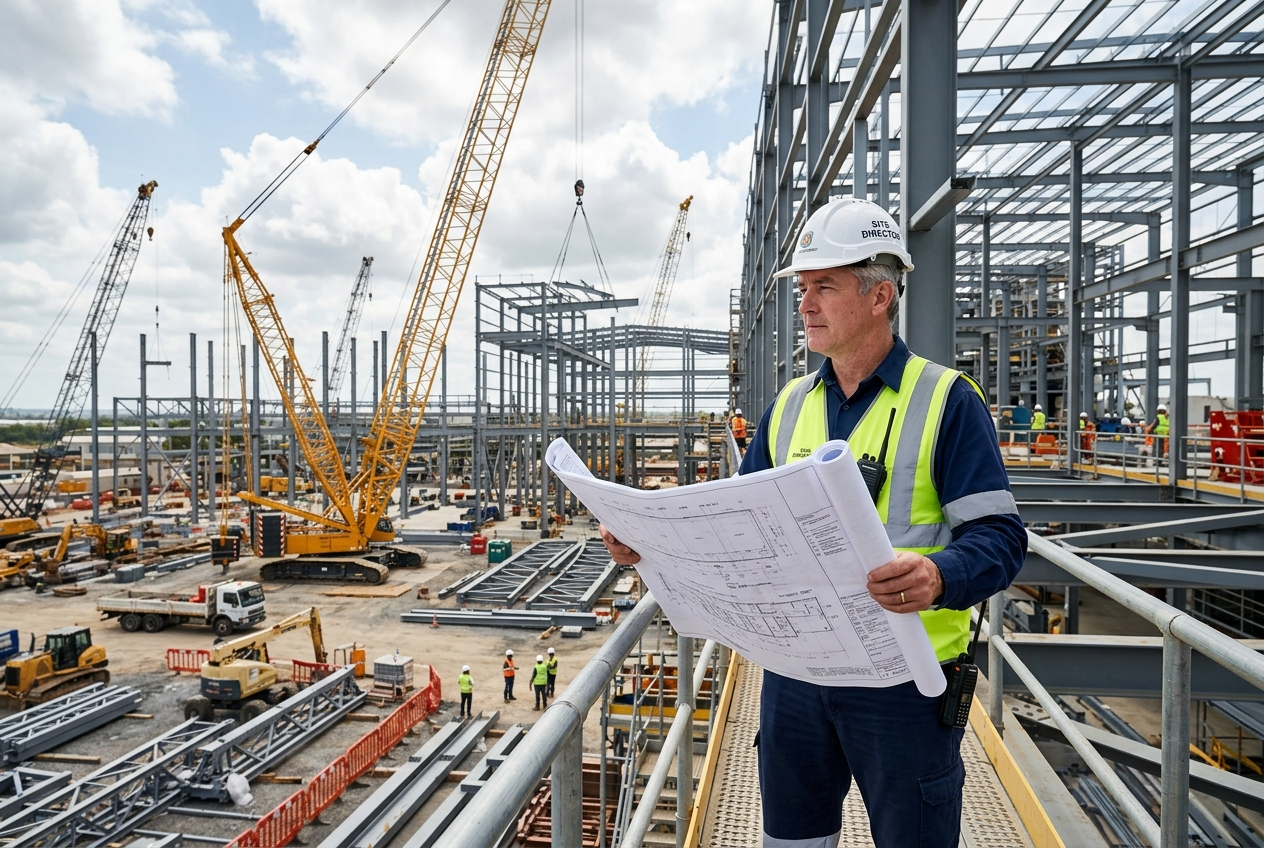
\includegraphics[height=70mm]{../../public/c_level_site_inspection.jpg}};
  \end{scope}
  \draw[white!45!gray,rounded corners=2pt,line width=.6pt] (126,16) rectangle (179,86);
  \fill[TTCBlue] (126,7) rectangle (179,15);
  \node[text=white,font=\fontsize{6.4}{7.5}\selectfont\bfseries] at (152.5,11)
    {管理层一线巡检现场};
\end{tikzpicture}

\vspace{3mm}

\noindent
\begin{tikzpicture}[x=1mm,y=1mm]
  \path[use as bounding box] (0,0) rectangle (186,49);
  \fill[white,rounded corners=3pt] (0,0) rectangle (186,49);
  \draw[TTCBorder,rounded corners=3pt,line width=.6pt] (0,0) rectangle (186,49);
  \node[anchor=west,text=TTCBlue,font=\fontsize{8}{9.5}\selectfont\bfseries] at (7,41)
    {\faMobile*\quad 赋能业主与监理透明决策};
  \foreach \x in {62,124}{\draw[TTCBorder] (\x,7) -- (\x,33);}
  \node[anchor=north west,text width=50mm] at (6,31) {
    {\fontsize{8}{9.5}\selectfont\bfseries\color{TTCRed} 劳务出勤透明}\\[.7mm]
    {\fontsize{6.6}{8}\selectfont\color{TTCTextDark}
    实时掌握在场工人总数、工种分布与特殊工种资格状态。}
  };
  \node[anchor=north west,text width=50mm] at (68,31) {
    {\fontsize{8}{9.5}\selectfont\bfseries\color{TTCCyan} 安全态势可视化}\\[.7mm]
    {\fontsize{6.6}{8}\selectfont\color{TTCTextDark}
    未戴安全帽/反光背心等违规行为自动抓拍并推送整改。}
  };
  \node[anchor=north west,text width=50mm] at (130,31) {
    {\fontsize{8}{9.5}\selectfont\bfseries\color{TTCGold} 验收档案完备}\\[.7mm]
    {\fontsize{6.6}{8}\selectfont\color{TTCTextDark}
    电子日志、RFI与ITP检验记录带时间戳与数字签名可追溯。}
  };
\end{tikzpicture}

\vspace{3mm}

\noindent
\begin{tikzpicture}[x=1mm,y=1mm]
  \path[use as bounding box] (0,0) rectangle (186,43);
  \fill[TTCLightBlue,rounded corners=3pt] (0,0) rectangle (186,43);
  \draw[TTCBorder,rounded corners=3pt,line width=.6pt] (0,0) rectangle (186,43);
  \node[anchor=west,text=TTCBlue,font=\fontsize{8}{9.5}\selectfont\bfseries] at (7,35)
    {\faCheckCircle\quad 每日数字化管理执行闭环};
  \foreach \x/\n/\t in {23/01/数据采集,69/02/智能预警,115/03/现场处置,161/04/归档留痕}{
    \fill[white] (\x,17) circle (5);
    \draw[TTCBlue,line width=.8pt] (\x,17) circle (5);
    \node[text=TTCRed,font=\fontsize{6.3}{7}\selectfont\bfseries] at (\x,17) {\n};
    \node[anchor=north,align=center,text width=34mm] at (\x,9)
      {{\fontsize{6.7}{8}\selectfont\bfseries\color{TTCBlue} \t}};
  }
  \draw[-{Stealth[length=2mm]},TTCBlue!45!white,line width=.9pt] (29,17) -- (63,17);
  \draw[-{Stealth[length=2mm]},TTCBlue!45!white,line width=.9pt] (75,17) -- (109,17);
  \draw[-{Stealth[length=2mm]},TTCBlue!45!white,line width=.9pt] (121,17) -- (155,17);
\end{tikzpicture}
\end{minipage}
\newpage

% ============================================================
% TRANG 18: QUALITY PASSPORT & RELEASE GATES
% ============================================================
\pageheaderbar{全面QA/QC质量体系与AWS D1.1标准}{第18页}
\pagefooterbar{第18页}

\begin{tikzpicture}[remember picture, overlay]
  \fill[TTCLightBlue]
    ([xshift=121mm,yshift=-31mm]current page.north west) --
    ([xshift=210mm,yshift=-31mm]current page.north west) --
    ([xshift=210mm,yshift=-118mm]current page.north west) -- cycle;
  \begin{scope}[shift={(current page.south west)},x=1mm,y=1mm,opacity=.43]
    \draw[TTCBlue!17!white,line width=.7pt] (14,15) -- (196,15);
    \foreach \x in {18,56,94,132,170}{
      \draw[TTCBlue!15!white,rounded corners=1pt] (\x,15) rectangle +(25,28);
      \draw[TTCRed!14!white] (\x+5,35) -- (\x+20,35);
      \draw[TTCBlue!11!white] (\x+5,29) -- (\x+20,29);
      \draw[TTCBlue!11!white] (\x+5,23) -- (\x+16,23);
    }
  \end{scope}
\end{tikzpicture}

\begin{minipage}[t][246mm]{\textwidth}
\secbrand{各专业分项工程质量通行证体系}{4级 ITP 严格受控 • 凭齐备数据凭据逐级放行}

{\fontsize{15}{17}\selectfont\bfseries\color{TTCBlue}
凭充分检验凭据方可转入下一道工序\par}
\vspace{1mm}
{\fontsize{7.5}{9}\selectfont\color{TTCTextMuted}
每批原材料、每条焊缝及每道分项工程均须经过检验、签署并归档，方可放行进入下一道工序。\par}
\vspace{3mm}

\noindent
\begin{tikzpicture}[x=1mm,y=1mm]
  \path[use as bounding box] (0,0) rectangle (186,122);

  % Left ladder
  \fill[TTCDeepNavy,rounded corners=3pt] (0,0) rectangle (57,122);
  \node[anchor=west,text=TTCCyan,font=\fontsize{7}{8}\selectfont\bfseries] at (6,113)
    {4 级品控管理};
  \node[anchor=west,text=white,font=\fontsize{11}{12}\selectfont\bfseries] at (6,106.5)
    {ITP 检验关口};

  \foreach \y/\n/\c in {78/01/TTCRed,52/02/TTCBlue,26/03/TTCCyan,0/04/TTCGold}{
    \fill[white,rounded corners=2pt] (6,\y+6) rectangle (51,\y+25);
    \draw[\c,rounded corners=2pt,line width=.7pt] (6,\y+6) rectangle (51,\y+25);
    \fill[\c] (6,\y+6) rectangle (13,\y+25);
    \node[text=white,font=\fontsize{6.5}{7}\selectfont\bfseries] at (9.5,\y+15.5) {\n};
  }
  \node[anchor=west,text width=33mm] at (16,93.5) {
    {\fontsize{7.2}{8.5}\selectfont\bfseries\color{TTCRed} 班组自检}\\[-.2mm]
    {\fontsize{6.2}{7.4}\selectfont\color{TTCTextMuted}内部自查与交接单}
  };
  \node[anchor=west,text width=33mm] at (16,67.5) {
    {\fontsize{7.2}{8.5}\selectfont\bfseries\color{TTCBlue} 专业工程师复核}\\[-.2mm]
    {\fontsize{6.2}{7.4}\selectfont\color{TTCTextMuted}对照施工图纸与ITP}
  };
  \node[anchor=west,text width=33mm] at (16,41.5) {
    {\fontsize{7.2}{8.5}\selectfont\bfseries\color{TTCCyan} 独立专职 QA/QC}\\[-.2mm]
    {\fontsize{6.2}{7.4}\selectfont\color{TTCTextMuted}NDT报告与试验数据}
  };
  \node[anchor=west,text width=33mm] at (16,15.5) {
    {\fontsize{7.2}{8.5}\selectfont\bfseries\color{TTCGold} 监理 / 业主确认}\\[-.2mm]
    {\fontsize{6.2}{7.4}\selectfont\color{TTCTextMuted}最终签字验收放行}
  };
  \draw[-{Stealth[length=2mm]},white!55!gray,line width=.8pt] (28.5,83) -- (28.5,78);
  \draw[-{Stealth[length=2mm]},white!55!gray,line width=.8pt] (28.5,57) -- (28.5,52);
  \draw[-{Stealth[length=2mm]},white!55!gray,line width=.8pt] (28.5,31) -- (28.5,26);

  % Right passport
  \fill[white,rounded corners=3pt] (62,0) rectangle (186,122);
  \draw[TTCBorder,rounded corners=3pt,line width=.7pt] (62,0) rectangle (186,122);
  \fill[TTCLightBlue,rounded corners=3pt] (62,101) rectangle (186,122);
  \node[anchor=west,text=TTCBlue,font=\fontsize{10}{11.5}\selectfont\bfseries] at (68,113)
    {\faClipboardCheck\quad 分项工程质量通行证};
  \node[anchor=east,text=TTCTextMuted,font=\fontsize{6}{7}\selectfont\bfseries] at (180,113)
    {任务包代码 / 全程追溯};

  \foreach \y/\n/\c in {78/01/TTCRed,55/02/TTCBlue,32/03/TTCCyan,9/04/TTCGold}{
    \fill[\c!6!white,rounded corners=1.5pt] (68,\y) rectangle (180,\y+18);
    \node[anchor=west,text=\c,font=\fontsize{7}{8}\selectfont\bfseries] at (72,\y+12) {\n};
    \fill[\c] (165,\y+5) circle (2.3);
    \node[text=white,font=\fontsize{5}{5.5}\selectfont\bfseries] at (165,\y+5) {\faCheck};
    \node[anchor=west,text=TTCTextMuted,font=\fontsize{6.1}{7.2}\selectfont\bfseries] at (170,\y+5) {合格};
  }
  \node[anchor=west,text=TTCBlue,font=\fontsize{7.4}{8.7}\selectfont\bfseries] at (81,90) {原材料质量溯源};
  \node[anchor=west,text=TTCTextDark,font=\fontsize{6.3}{7.5}\selectfont] at (81,84) {CO/CQ 原产地证明 • 炉批号 • 出厂质保书 • 进场复验报告};
  \node[anchor=west,text=TTCBlue,font=\fontsize{7.4}{8.7}\selectfont\bfseries] at (81,67) {钢构焊接工艺控制};
  \node[anchor=west,text=TTCTextDark,font=\fontsize{6.3}{7.5}\selectfont] at (81,61) {WPS/PQR 规程 • 焊工钢印 • 美国 AWS D1.1 • 焊缝追踪排布图};
  \node[anchor=west,text=TTCBlue,font=\fontsize{7.4}{8.7}\selectfont\bfseries] at (81,44) {无损探伤无缝检验};
  \node[anchor=west,text=TTCTextDark,font=\fontsize{6.3}{7.5}\selectfont] at (81,38) {外观VT • 超声UT • 磁粉MT/渗透PT • 第三方检测机构报告};
  \node[anchor=west,text=TTCBlue,font=\fontsize{7.4}{8.7}\selectfont\bfseries] at (81,21) {竣工档案与数字闭环};
  \node[anchor=west,text=TTCTextDark,font=\fontsize{6.3}{7.5}\selectfont] at (81,15) {签署ITP检验批 • 闭环NCR • 竣工图纸 • CDE云端永久留存};
\end{tikzpicture}

\vspace{3mm}

\noindent
\begin{tikzpicture}[x=1mm,y=1mm]
  \path[use as bounding box] (0,0) rectangle (186,46);
  \fill[TTCLightBlue,rounded corners=3pt] (0,0) rectangle (186,46);
  \draw[TTCBorder,rounded corners=3pt,line width=.6pt] (0,0) rectangle (186,46);
  \node[anchor=west,text=TTCBlue,font=\fontsize{8}{9.5}\selectfont\bfseries] at (7,38)
    {\faCheckDouble\quad NDT 无损探伤与物理力学检测方法};
  \foreach \x in {46.5,93,139.5}{\draw[TTCBorder] (\x,6) -- (\x,31);}
  \node[align=center,text width=38mm] at (23.25,18) {
    {\fontsize{9}{10}\selectfont\bfseries\color{TTCRed} VT 目视检测}\\[-.2mm]
    {\fontsize{6.1}{7.3}\selectfont 几何尺寸 • 咬边 • 焊脚高度}
  };
  \node[align=center,text width=38mm] at (69.75,18) {
    {\fontsize{9}{10}\selectfont\bfseries\color{TTCCyan} UT 超声探伤}\\[-.2mm]
    {\fontsize{6.3}{7.5}\selectfont 内部夹渣 • 气孔 • 未熔合}
  };
  \node[align=center,text width=38mm] at (116.25,18) {
    {\fontsize{9}{10}\selectfont\bfseries\color{TTCBlue} MT / PT 磁粉渗透}\\[-.2mm]
    {\fontsize{6.3}{7.5}\selectfont 表面微裂纹与角焊缝缺陷}
  };
  \node[align=center,text width=38mm] at (162.75,18) {
    {\fontsize{9}{10}\selectfont\bfseries\color{TTCGold} LAS-XD 试验室}\\[-.2mm]
    {\fontsize{6.3}{7.5}\selectfont 国家资质试验室力学拉拔}
  };
\end{tikzpicture}

\vspace{3mm}

\noindent
\begin{tikzpicture}[x=1mm,y=1mm]
  \path[use as bounding box] (0,0) rectangle (186,30);
  \fill[TTCDeepNavy,rounded corners=3pt] (0,0) rectangle (186,30);
  \node[anchor=west,text=TTCCyan,font=\fontsize{7}{8}\selectfont\bfseries] at (8,20)
    {质量放行铁律};
  \node[anchor=west,text=white,font=\fontsize{10}{11.5}\selectfont\bfseries] at (8,11)
    {检验合格 → 数据齐全 → 签字核准 → 全程可溯};
  \node[anchor=east,text=TTCGold,font=\fontsize{12}{13}\selectfont\bfseries] at (178,15)
    {AWS D1.1 • ISO 9001};
\end{tikzpicture}
\end{minipage}
\newpage

% ============================================================
% TRANG 19: HSE DECISION SYSTEM & STOP WORK AUTHORITY
% ============================================================
\pageheaderbar{HSE职业健康安全与零事故文化}{第19页}
\pagefooterbar{第19页}

\begin{tikzpicture}[remember picture, overlay]
  \fill[TTCRed!4!white]
    ([xshift=0mm,yshift=-210mm]current page.north west) --
    ([xshift=67mm,yshift=-248mm]current page.north west) --
    ([xshift=0mm,yshift=-278mm]current page.north west) -- cycle;
  \fill[TTCLightBlue]
    ([xshift=148mm,yshift=-31mm]current page.north west) --
    ([xshift=210mm,yshift=-31mm]current page.north west) --
    ([xshift=210mm,yshift=-108mm]current page.north west) -- cycle;
  \node[opacity=.035,text=TTCRed,font=\fontsize{66}{68}\selectfont\bfseries,
        rotate=90] at ([xshift=-11mm,yshift=-2mm]current page.east) {STOP};
\end{tikzpicture}

\begin{minipage}[t][246mm]{\textwidth}
\secbrand{安全是一套严密的管理决策机制 — 不仅仅是劳保装备}{Risk Elimination, Daily Control Cycle \& Stop Work Authority}

{\fontsize{15}{17}\selectfont\bfseries\color{TTCBlue}
洞察隐患 • 事前管控 • 遇险立即行使停工权\par}
\vspace{1mm}
{\fontsize{7.5}{9}\selectfont\color{TTCTextMuted}
工期进度绝不能成为容忍不安全作业环境的借口；人的生命安全永远高于一切。\par}
\vspace{3mm}

\noindent
\begin{tikzpicture}[x=1mm,y=1mm]
  \path[use as bounding box] (0,0) rectangle (186,149);

  % Left manifesto
  \fill[TTCDeepNavy,rounded corners=3pt] (0,0) rectangle (58,149);
  \begin{scope}
    \clip[rounded corners=3pt] (0,87) rectangle (58,149);
    \node[anchor=center,inner sep=0pt] at (29,118)
      {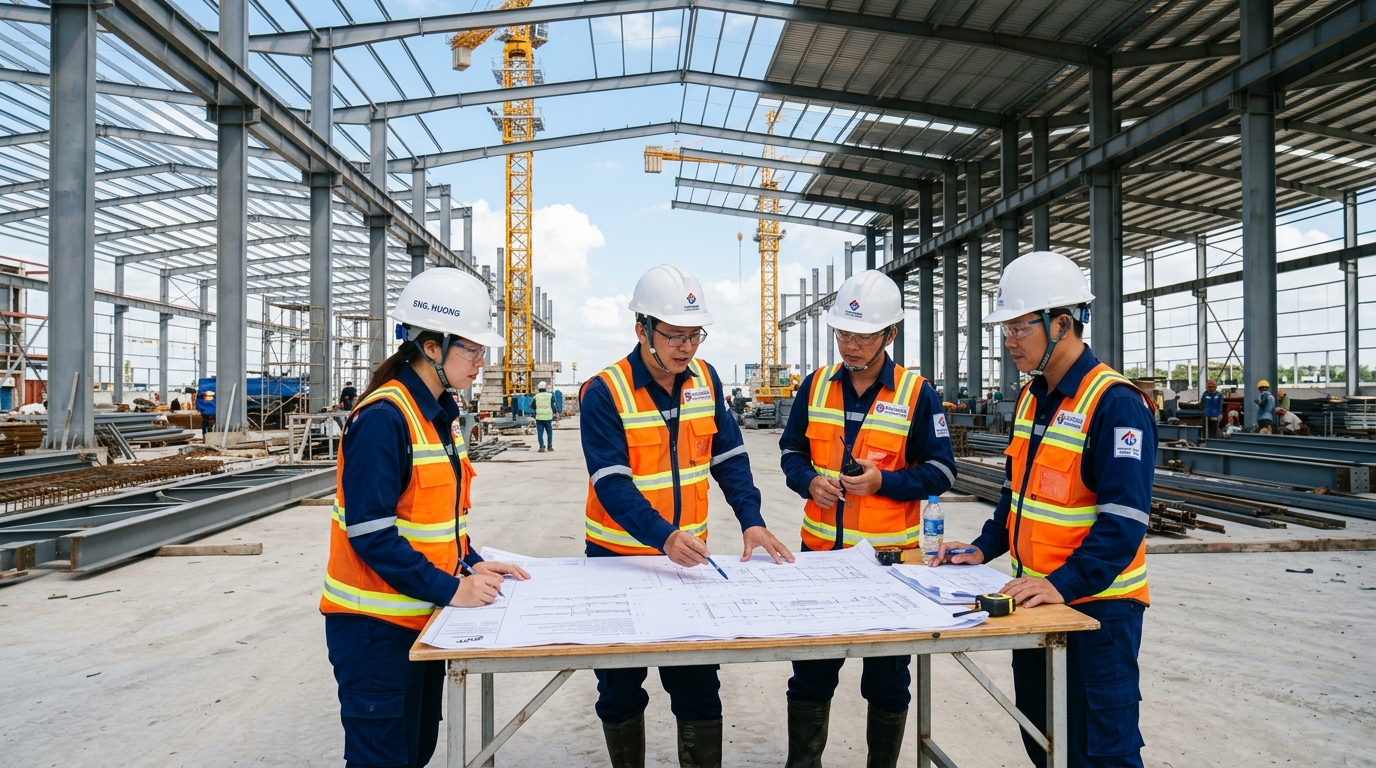
\includegraphics[height=62mm]{../../public/engineer-team-site.jpg}};
    \fill[TTCDeepNavy,opacity=.28] (0,87) rectangle (58,149);
  \end{scope}
  \node[anchor=west,text=TTCCyan,font=\fontsize{7}{8}\selectfont\bfseries] at (7,78)
    {STOP WORK AUTHORITY};
  \node[anchor=west,text=white,font=\fontsize{22}{23}\selectfont\bfseries] at (7,63)
    {STOP};
  \node[anchor=west,text=TTCRed!85!white,font=\fontsize{22}{23}\selectfont\bfseries] at (7,48)
    {WORK};
  \node[anchor=north west,text width=44mm,align=left] at (7,37) {
    {\fontsize{6.8}{8.3}\selectfont\color{white!85!gray}
    任何员工在发现安全条件不具备时，均有权且必须立即下达停工指令。}\\[2mm]
    {\fontsize{7}{8.5}\selectfont\bfseries\color{TTCGold}
    生命安全高于一切生产效益}
  };

  % Right — hierarchy of controls
  \fill[white,rounded corners=3pt] (63,86) rectangle (186,149);
  \draw[TTCBorder,rounded corners=3pt,line width=.6pt] (63,86) rectangle (186,149);
  \node[anchor=west,text=TTCBlue,font=\fontsize{8}{9.5}\selectfont\bfseries] at (69,141)
    {\faShield*\quad 风险控制四级优先层级};

  \fill[TTCRed] (69,124) rectangle (180,136);
  \fill[TTCBlue] (74,111) rectangle (175,123);
  \fill[TTCCyan] (79,98) rectangle (170,110);
  \fill[TTCGold] (84,85) rectangle (165,97);
  \node[anchor=west,text=white,font=\fontsize{7}{8}\selectfont\bfseries] at (73,130) {01 • 消除 (ELIMINATE) — 优化工艺从源头根除危险};
  \node[anchor=west,text=white,font=\fontsize{7}{8}\selectfont\bfseries] at (78,117) {02 • 工程防护 (ENGINEER) — 临边护栏、安全网与生命线};
  \node[anchor=west,text=white,font=\fontsize{7}{8}\selectfont\bfseries] at (83,104) {03 • 管理许可 (PERMIT) — JSA风险分析与动火作业票};
  \node[anchor=west,text=white,font=\fontsize{7}{8}\selectfont\bfseries] at (88,91) {04 • 劳保防护 (PPE) — 个人最后一道被动安全屏障};

  % Right — daily cycle
  \fill[TTCLightBlue,rounded corners=3pt] (63,29) rectangle (186,81);
  \draw[TTCBorder,rounded corners=3pt,line width=.6pt] (63,29) rectangle (186,81);
  \node[anchor=west,text=TTCBlue,font=\fontsize{8}{9.5}\selectfont\bfseries] at (69,73)
    {\faClock\quad 每日安全闭环控制流程};
  \draw[TTCBlue!35!white,line width=1pt] (76,50) -- (175,50);
  \foreach \x/\n/\t in {77/01/策划,102/02/交底,127/03/核查,152/04/作业,175/05/收工}{
    \fill[white] (\x,50) circle (4.5);
    \draw[TTCBlue,line width=.75pt] (\x,50) circle (4.5);
    \node[text=TTCRed,font=\fontsize{5.8}{6.5}\selectfont\bfseries] at (\x,50) {\n};
    \node[anchor=north,align=center,text width=22mm] at (\x,42)
      {{\fontsize{6}{7.2}\selectfont\bfseries\color{TTCBlue} \t}};
  }
  \node[anchor=west,text=TTCTextMuted,font=\fontsize{6}{7.3}\selectfont] at (70,33)
    {JSA安全分析 → 班前会 (Toolbox) → 装备核查 → 旁站监督 → 现场清场};

  % Emergency row
  \fill[white,rounded corners=3pt] (63,0) rectangle (186,24);
  \draw[TTCBorder,rounded corners=3pt,line width=.6pt] (63,0) rectangle (186,24);
  \node[anchor=west,text=TTCRed,font=\fontsize{8}{9.5}\selectfont\bfseries] at (69,16)
    {\faFireExtinguisher\quad 应急响应保障机制};
  \node[anchor=west,text=TTCTextDark,font=\fontsize{6.4}{7.8}\selectfont] at (69,7)
    {即时警报 • 隔离现场 • 紧急疏散 • 现场急救 • 事故溯源调查 • 制定防范措施};
\end{tikzpicture}

\vspace{3mm}

\noindent
\begin{tikzpicture}[x=1mm,y=1mm]
  \path[use as bounding box] (0,0) rectangle (186,48);
  \fill[white,rounded corners=3pt] (0,0) rectangle (186,48);
  \draw[TTCBorder,rounded corners=3pt,line width=.6pt] (0,0) rectangle (186,48);
  \node[anchor=west,text=TTCBlue,font=\fontsize{8}{9.5}\selectfont\bfseries] at (7,40)
    {\faHandPaper\quad 现场五大保命安全法则};
  \foreach \x in {37.2,74.4,111.6,148.8}{\draw[TTCBorder] (\x,6) -- (\x,31);}
  \node[align=center,text width=32mm] at (18.6,18) {
    {\fontsize{7.3}{8.5}\selectfont\bfseries\color{TTCRed} 高空作业}\\[-.2mm]
    {\fontsize{5.8}{7}\selectfont 双大钩 • 生命绳 • 防坠网}
  };
  \node[align=center,text width=32mm] at (55.8,18) {
    {\fontsize{7.3}{8.5}\selectfont\bfseries\color{TTCBlue} 起重吊装}\\[-.2mm]
    {\fontsize{5.8}{7}\selectfont 警戒区 • 专职指挥 • 吊具核验}
  };
  \node[align=center,text width=32mm] at (93,18) {
    {\fontsize{7.3}{8.5}\selectfont\bfseries\color{TTCCyan} 施工用电}\\[-.2mm]
    {\fontsize{5.8}{7}\selectfont 漏保开关 • 可靠接地 • 上锁挂牌}
  };
  \node[align=center,text width=32mm] at (130.2,18) {
    {\fontsize{7.3}{8.5}\selectfont\bfseries\color{TTCGold} 动火作业}\\[-.2mm]
    {\fontsize{5.8}{7}\selectfont 专人看火 • 灭火器材 • 动火票}
  };
  \node[align=center,text width=32mm] at (167.4,18) {
    {\fontsize{7.3}{8.5}\selectfont\bfseries\color{TTCBlue} 基坑开挖}\\[-.2mm]
    {\fontsize{5.8}{7}\selectfont 规范放坡 • 临边护栏 • 逃生通道}
  };
\end{tikzpicture}
\end{minipage}
\newpage

% ============================================================
% TRANG 20: SỔ DANH MỤC DỰ ÁN TIÊU BIỂU 01--08
% ============================================================
\AddToShipoutPictureFG*{%
  \AtPageUpperLeft{%
    \begin{tikzpicture}[x=1mm,y=1mm]
      \path[use as bounding box] (0,0) rectangle (0,0);
      \fill[TTCDeepNavy] (0,0) rectangle (210,-10);
      \fill[TTCRed] (0,-10) rectangle (210,-11);
      \node[anchor=west,text=white,font=\fontsize{7.5}{9}\selectfont\bfseries] at (12,-5)
        {\faBuilding\quad 新成功建筑科技股份公司 \textbullet\ TTC JSC};
      \node[anchor=east,text=TTCCyan,font=\fontsize{7.5}{9}\selectfont\bfseries] at (198,-5)
        {重点工业项目清单 • 01--08};
    \end{tikzpicture}%
  }%
  \AtPageLowerLeft{%
    \begin{tikzpicture}[x=1mm,y=1mm]
      \path[use as bounding box] (0,0) rectangle (0,0);
      \fill[TTCDeepNavy] (0,0) rectangle (210,8);
      \fill[TTCCyan] (0,8) rectangle (210,8.8);
      \node[anchor=west,text=white,font=\fontsize{6.8}{8}\selectfont] at (12,4)
        {\faPhone*\ +84 976 447 766 \quad\textbullet\quad \faEnvelope\ info@tanthanhcongjsc.com \quad\textbullet\quad \faGlobe\ https://tanthanhcongjsc.com};
      \node[anchor=east,text=white,font=\fontsize{7}{8}\selectfont\bfseries] at (198,4)
        {第20页};
    \end{tikzpicture}%
  }%
}

\begin{minipage}[t][246mm]{\textwidth}
\secbrand{重点工业建筑工程项目清单}{八座代表性工业工程 • 关键参数明晰 • 易于查阅核对}

{\fontsize{15}{17}\selectfont\bfseries\color{TTCBlue}
工程规模 • 建设地点 • TTC 承包履约范围\par}
\vspace{1mm}
{\fontsize{7.5}{9}\selectfont\color{TTCTextMuted}
项目清单按统一技术框架编排，便于业主迅速了解 TTC 在各个大型项目中的总包角色与核心贡献。\par}
\vspace{3mm}

\noindent
\begin{tikzpicture}[x=1mm,y=1mm]
  \path[use as bounding box] (0,0) rectangle (186,188);
  \fill[white,rounded corners=3pt] (0,0) rectangle (186,188);
  \draw[TTCBorder,rounded corners=3pt,line width=.7pt] (0,0) rectangle (186,188);

  % 表头
  \fill[TTCDeepNavy,rounded corners=3pt] (0,176) rectangle (186,188);
  \node[text=white,font=\fontsize{6.5}{7.5}\selectfont\bfseries] at (5,182) {序号};
  \node[anchor=west,text=white,font=\fontsize{6.5}{7.5}\selectfont\bfseries] at (14,182) {工程项目 / 投资业主};
  \node[text=white,font=\fontsize{6.5}{7.5}\selectfont\bfseries] at (84,182) {建筑规模};
  \node[anchor=west,text=white,font=\fontsize{6.5}{7.5}\selectfont\bfseries] at (96,182) {建设地点};
  \node[anchor=west,text=white,font=\fontsize{6.5}{7.5}\selectfont\bfseries] at (129,182) {TTC 承包范围};

  \newcommand{\projectrowa}[8]{%
    \fill[#8] (0,{#1-11}) rectangle (186,{#1+11});
    \fill[TTCBlue] (0,{#1-11}) rectangle (10,{#1+11});
    \node[text=white,font=\fontsize{7}{8}\selectfont\bfseries] at (5,#1) {#2};
    \node[anchor=west,text width=53mm,align=left] at (14,#1) {
      {\fontsize{7.2}{8.4}\selectfont\bfseries\color{TTCBlue} #3}\\[-.2mm]
      {\fontsize{5.8}{7}\selectfont\color{TTCTextMuted} #4}
    };
    \node[align=center,text width=20mm] at (84,#1)
      {{\fontsize{7}{8.2}\selectfont\bfseries\color{TTCTextDark} #5}};
    \node[anchor=west,text width=29mm,align=left] at (96,#1)
      {{\fontsize{5.9}{7.1}\selectfont\color{TTCTextDark} #6}};
    \node[anchor=west,text width=50mm,align=left] at (129,#1)
      {{\fontsize{6}{7.2}\selectfont\color{TTCTextDark} #7}};
    \draw[TTCBorder,line width=.45pt] (10,{#1-11}) -- (186,{#1-11});
  }

  \projectrowa{165}{01}{鸿庄制砖工厂综合体}{鸿庄股份公司 • 越南}{100,000 m$^2$}{永福省\\立石县}{EPC总承包 • 6.5个月快速交付}{TTCLightBlue}
  \projectrowa{143}{02}{红河第七制衣厂}{红河制衣集团 • 越南}{68,000 m$^2$}{南定省\\海后县}{设计与施工 • 双层重载工业地坪}{white}
  \projectrowa{121}{03}{Japfa Comfeed 饲料厂}{Japfa 集团 • 印度尼西亚}{50,000 m$^2$}{永福省\\太平省}{45米高耸筒仓群 • 精密车间}{TTCLightBlue}
  \projectrowa{99}{04}{正大 CP 饲料生产厂}{正大集团 • 泰国}{35,000 m$^2$}{河南省\\同文工业区}{重载生产车间 • 自动化恒温仓库}{white}
  \projectrowa{77}{05}{大润科技 DAEYUN 厂房}{大润集团 • 韩国}{20,000 m$^2$}{永福省\\霸善二期工业区}{Class 10,000无尘车间 • ESD防静电地坪}{TTCLightBlue}
  \projectrowa{55}{06}{住友电工 SUMIDENSO 线束厂}{住友电工 • 日本}{15,015 m$^2$}{后江省\\后江工业区}{汽车线束厂房 • 国际标准消防与水处理}{white}
  \projectrowa{33}{07}{富士康 FOXCONN 生产车间}{富士康科技集团 • 中国台湾}{12,000 m$^2$}{北宁省\\桂武工业区}{大跨度钢结构 • 高层工业厂房安装}{TTCLightBlue}
  \projectrowa{11}{08}{BW 工业智慧物流仓储}{BW Industrial • 新加坡}{45,000 m$^2$}{北宁省\\安丰工业区}{智慧物流仓储总包 • 超平地坪}{white}
\end{tikzpicture}

\vspace{3mm}

\noindent
\begin{tikzpicture}[x=1mm,y=1mm]
  \path[use as bounding box] (0,0) rectangle (186,35);
  \fill[TTCDeepNavy,rounded corners=3pt] (0,0) rectangle (186,35);
  \node[anchor=west,text=TTCCyan,font=\fontsize{6.2}{7.2}\selectfont\bfseries]
    at (7,29) {经大型工程检验的核心能力矩阵};
  \foreach \x in {46.5,93,139.5}{\draw[white!25!gray] (\x,5) -- (\x,23);}
  \node[align=center,text width=40mm] at (23.25,14) {
    {\fontsize{8.2}{9.5}\selectfont\bfseries\color{white} EPC / 设计施工一体化}\\[-.2mm]
    {\fontsize{5.9}{7.1}\selectfont\color{white!75!gray}单一责任主体贯穿全程}
  };
  \node[align=center,text width=40mm] at (69.75,14) {
    {\fontsize{8.2}{9.5}\selectfont\bfseries\color{white} 结构与 PEB 制造}\\[-.2mm]
    {\fontsize{5.9}{7.1}\selectfont\color{white!75!gray}大跨度 • 重荷载 • 筒仓}
  };
  \node[align=center,text width=40mm] at (116.25,14) {
    {\fontsize{8.2}{9.5}\selectfont\bfseries\color{white} 特种工业地坪}\\[-.2mm]
    {\fontsize{5.9}{7.1}\selectfont\color{white!75!gray}重载地坪 • 超平地坪}
  };
  \node[align=center,text width=40mm] at (162.75,14) {
    {\fontsize{8.2}{9.5}\selectfont\bfseries\color{white} 机电 MEP / 消防}\\[-.2mm]
    {\fontsize{5.9}{7.1}\selectfont\color{white!75!gray}基于工艺需求深度集成}
  };
\end{tikzpicture}
\end{minipage}
\newpage

% ============================================================
% TRANG 21: SỔ DANH MỤC DỰ ÁN TIÊU BIỂU 09--16
% ============================================================
\noindent\mbox{}\par\vspace{-\baselineskip}
\pageheaderbar{重点工业项目清单 • 09--16}{第21页}
\pagefooterbar{第21页}

\begin{minipage}[t][246mm]{\textwidth}
\secbrand{国际 FDI 及配套工业代表性项目清单}{八座标杆工程 • 跨国投资企业 • 专业严苛标准}

{\fontsize{15}{17}\selectfont\bfseries\color{TTCBlue}
跨国业主 • 行业领域 • EPC 解决方案\par}
\vspace{1mm}
{\fontsize{7.5}{9}\selectfont\color{TTCTextMuted}
全面展示 TTC 在食品加工、精密电子、机械制造、智慧物流及新能源领域的总包实战业绩。\par}
\vspace{3mm}

\noindent
\begin{tikzpicture}[x=1mm,y=1mm]
  \path[use as bounding box] (0,0) rectangle (186,188);
  \fill[white,rounded corners=3pt] (0,0) rectangle (186,188);
  \draw[TTCBorder,rounded corners=3pt,line width=.7pt] (0,0) rectangle (186,188);

  \fill[TTCDeepNavy,rounded corners=3pt] (0,176) rectangle (186,188);
  \node[text=white,font=\fontsize{6.5}{7.5}\selectfont\bfseries] at (5,182) {序号};
  \node[anchor=west,text=white,font=\fontsize{6.5}{7.5}\selectfont\bfseries] at (14,182) {工程项目 / 投资业主};
  \node[text=white,font=\fontsize{6.5}{7.5}\selectfont\bfseries] at (84,182) {建筑规模};
  \node[anchor=west,text=white,font=\fontsize{6.5}{7.5}\selectfont\bfseries] at (96,182) {建设地点};
  \node[anchor=west,text=white,font=\fontsize{6.5}{7.5}\selectfont\bfseries] at (129,182) {TTC 承包范围};

  \newcommand{\projectrowb}[8]{%
    \fill[#8] (0,{#1-11}) rectangle (186,{#1+11});
    \fill[TTCBlue] (0,{#1-11}) rectangle (10,{#1+11});
    \node[text=white,font=\fontsize{7}{8}\selectfont\bfseries] at (5,#1) {#2};
    \node[anchor=west,text width=53mm,align=left] at (14,#1) {
      {\fontsize{7.2}{8.4}\selectfont\bfseries\color{TTCBlue} #3}\\[-.2mm]
      {\fontsize{5.8}{7}\selectfont\color{TTCTextMuted} #4}
    };
    \node[align=center,text width=20mm] at (84,#1)
      {{\fontsize{7}{8.2}\selectfont\bfseries\color{TTCTextDark} #5}};
    \node[anchor=west,text width=29mm,align=left] at (96,#1)
      {{\fontsize{5.9}{7.1}\selectfont\color{TTCTextDark} #6}};
    \node[anchor=west,text width=50mm,align=left] at (129,#1)
      {{\fontsize{6}{7.2}\selectfont\color{TTCTextDark} #7}};
    \draw[TTCBorder,line width=.45pt] (10,{#1-11}) -- (186,{#1-11});
  }

  \projectrowb{165}{09}{新希望 NEW HOPE 饲料厂}{新希望六和 • 新加坡/中国}{32,000 m$^2$}{北江省\\光州工业区}{粮食筒仓群 • 22kV变电站及重载道路}{TTCLightBlue}
  \projectrowb{143}{10}{新城 SHINJO 精密机械厂}{Shinjo 精密 • 日本}{18,500 m$^2$}{北宁省\\VSIP 工业区}{精密机加工车间 • 15T行车梁结构}{white}
  \projectrowb{121}{11}{东和田 TOWADA 电子厂}{Towada 电子 • 日本}{16,000 m$^2$}{海阳省\\福田工业区}{芯片精密贴片车间 • ISO无尘室}{TTCLightBlue}
  \projectrowb{99}{12}{东洋制罐 TOYO SEIKAN 厂房}{Toyo Seikan • 日本}{22,000 m$^2$}{北宁省\\仙山工业区}{EPC总承包 • 自动化包装车间 • 超平地坪}{white}
  \projectrowb{77}{13}{花美 FAMI 服饰制造厂}{Fami Garment • 韩国}{28,000 m$^2$}{富寿省\\瑞云工业区}{双层大型制衣厂房 • 工业暖通空调系统}{TTCLightBlue}
  \projectrowb{55}{14}{邮船 YUSEN 国际物流中心}{Yusen Logistics • 日本}{25,000 m$^2$}{海防市\\亭武工业区}{保税立体仓库 • 自动液压升降调节板}{white}
  \projectrowb{33}{15}{味王 A-ONE 食品生产基地}{味王股份 • 中国台湾}{30,000 m$^2$}{平阳省\\神浪二期工业区}{食品洁净加工车间 • HACCP标准系统}{TTCLightBlue}
  \projectrowb{11}{16}{山河 SON HA 新能源装备厂}{山河集团 • 越南}{24,000 m$^2$}{北宁省\\顺成工业区}{大型储罐车间 • 屋顶太阳能光伏系统}{white}
\end{tikzpicture}

\vspace{3mm}

\noindent
\begin{tikzpicture}[x=1mm,y=1mm]
  \path[use as bounding box] (0,0) rectangle (186,35);
  \fill[TTCDeepNavy,rounded corners=3pt] (0,0) rectangle (186,35);
  \node[anchor=west,text=TTCCyan,font=\fontsize{6.2}{7.2}\selectfont\bfseries]
    at (7,29) {精选 6 大经典工程案例深度剖析 • 第 22--27 页};
  \foreach \x in {62,124}{\draw[white!25!gray] (\x,5) -- (\x,23);}
  \node[align=center,text width=53mm] at (31,14) {
    {\fontsize{7.8}{9.2}\selectfont\bfseries\color{white} 鸿庄制砖 • 红河第七制衣}\\[-.2mm]
    {\fontsize{6}{7.2}\selectfont\color{white!75!gray}超大跨度EPC • 双层重载厂房}
  };
  \node[align=center,text width=53mm] at (93,14) {
    {\fontsize{7.8}{9.2}\selectfont\bfseries\color{white} JAPFA 饲料 • 大润科技}\\[-.2mm]
    {\fontsize{6.2}{7.2}\selectfont\color{white!75!gray}工艺装置高耸筒仓 • 无尘洁净室}
  };
  \node[align=center,text width=53mm] at (155,14) {
    {\fontsize{7.8}{9.2}\selectfont\bfseries\color{white} 住友电工 • 富士康}\\[-.2mm]
    {\fontsize{6}{7.2}\selectfont\color{white!75!gray}日系严苛品控 • 电子装配厂房}
  };
\end{tikzpicture}
\end{minipage}
\newpage

% ============================================================
% TRANG 22: FLAGSHIP CASE -- NHÀ MÁY GẠCH HỒNG TRANG
% ============================================================
\noindent\mbox{}\par\vspace{-\baselineskip}
\casepagebars{经典案例 • 鸿庄制砖工厂}{第22页}

\begin{minipage}[t][246mm]{\textwidth}
\secbrand{经典工程案例 01: 鸿庄制砖工厂综合体}{Flagship EPC case • Large-span industrial facility • Lập Thạch, Vĩnh Phúc}

\noindent
\begin{tikzpicture}[x=1mm,y=1mm]
  \path[use as bounding box] (0,0) rectangle (186,220);

  % 现场实景照片
  \begin{scope}
    \clip[rounded corners=4pt] (0,150) rectangle (70,220);
    \node[inner sep=0pt] at (35,185)
      {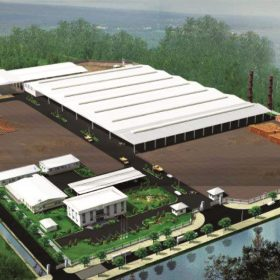
\includegraphics[width=70mm,height=70mm]{../../public/project-assets/hongtrang.jpg}};
    \fill[TTCDeepNavy,opacity=.88] (0,150) rectangle (70,161);
    \node[anchor=west,text=white,font=\fontsize{7}{8}\selectfont\bfseries]
      at (4,155.5) {工程实景 • 永福省立石县};
  \end{scope}
  \draw[TTCBorder,rounded corners=4pt,line width=.7pt] (0,150) rectangle (70,220);

  % 概况数据
  \fill[TTCLightBlue,rounded corners=4pt] (74,150) rectangle (186,220);
  \draw[TTCBorder,rounded corners=4pt,line width=.7pt] (74,150) rectangle (186,220);
  \node[anchor=north west,text=TTCRed,font=\fontsize{7.5}{9}\selectfont\bfseries]
    at (80,214) {EPC 总承包模式};
  \node[anchor=north west,text width=99mm,align=left,text=TTCBlue,
        font=\fontsize{14}{16}\selectfont\bfseries]
    at (80,207) {100,000 m$^2$ 规划总面积};
  \draw[TTCBorder,line width=.55pt] (80,190) -- (180,190);
  \foreach \x in {113.3,146.6}{\draw[TTCBorder,line width=.5pt] (\x,163) -- (\x,186);}
  \node[align=center,text width=29mm] at (96.5,176) {
    {\fontsize{11}{12}\selectfont\bfseries\color{TTCRed}75,000 m$^2$}\\[-.5mm]
    {\fontsize{6.2}{7.4}\selectfont\color{TTCTextMuted}车间建筑面积}};
  \node[align=center,text width=29mm] at (130,176) {
    {\fontsize{11}{12}\selectfont\bfseries\color{TTCBlue}跨度 42米}\\[-.5mm]
    {\fontsize{6.2}{7.4}\selectfont\color{TTCTextMuted}无中柱开敞空间}};
  \node[align=center,text width=29mm] at (163.5,176) {
    {\fontsize{11}{12}\selectfont\bfseries\color{TTCBlue}6.5 个月}\\[-.5mm]
    {\fontsize{6.2}{7.4}\selectfont\color{TTCTextMuted}快速完工交付}};
  \node[anchor=south west,text width=99mm,align=left,text=TTCTextDark,
        font=\fontsize{7.4}{9}\selectfont]
    at (80,153) {\textbf{TTC承包范围：} EPC总承包；统筹地质勘探、方案设计、PEB制造、重型地坪、机电及Fast-track快速施工。};

  % 案例故事
  \node[anchor=west,text=TTCBlue,font=\fontsize{8}{9.5}\selectfont\bfseries]
    at (0,143) {核心技术攻坚 • 挑战、方案与成效};

  \fill[white,rounded corners=4pt] (0,79) rectangle (58,137);
  \draw[TTCBorder,rounded corners=4pt,line width=.7pt] (0,79) rectangle (58,137);
  \fill[TTCRed,rounded corners=2pt] (5,124) rectangle (16,133);
  \node[text=white,font=\fontsize{7}{8}\selectfont\bfseries] at (10.5,128.5) {01};
  \node[anchor=north west,text=TTCBlue,font=\fontsize{9}{10.5}\selectfont\bfseries]
    at (5,120) {技术挑战};
  \node[anchor=north west,text width=48mm,align=left,text=TTCTextDark,
        font=\fontsize{7.2}{9}\selectfont]
    at (5,110) {窑炉连续生产线要求全长无立柱阻隔，柱网跨度达42米；同时超长车间须具备高效自然排烟散热能力。};

  \draw[-{Latex[length=2.5mm]},TTCCyan,line width=1pt] (59.5,108) -- (63,108);
  \fill[TTCDeepNavy,rounded corners=4pt] (64,79) rectangle (122,137);
  \node[text=TTCDeepNavy,fill=white,rounded corners=2pt,font=\fontsize{7}{8}\selectfont\bfseries,
        minimum width=11mm,minimum height=9mm] at (74.5,128.5) {02};
  \node[anchor=north west,text=white,font=\fontsize{9}{10.5}\selectfont\bfseries]
    at (69,120) {TTC 解决方案};
  \node[anchor=north west,text width=48mm,align=left,text=white,
        font=\fontsize{7.2}{9}\selectfont]
    at (69,110) {采用42米变截面高强门式刚架；屋脊设置通长自吸式通风气楼；设计、制造与土建各工序穿插并行。};

  \draw[-{Latex[length=2.5mm]},TTCCyan,line width=1pt] (123.5,108) -- (127,108);
  \fill[TTCLightBlue,rounded corners=4pt] (128,79) rectangle (186,137);
  \draw[TTCBorder,rounded corners=4pt,line width=.7pt] (128,79) rectangle (186,137);
  \fill[TTCBlue,rounded corners=2pt] (133,124) rectangle (144,133);
  \node[text=white,font=\fontsize{7}{8}\selectfont\bfseries] at (138.5,128.5) {03};
  \node[anchor=north west,text=TTCBlue,font=\fontsize{9}{10.5}\selectfont\bfseries]
    at (133,120) {交付成效};
  \node[anchor=north west,text width=48mm,align=left,text=TTCTextDark,
        font=\fontsize{7.2}{9}\selectfont]
    at (133,110) {仅历时6.5个月完成75,000 m$^2$建筑安装，比合同原定节点提前20天高品质交付投产。};

  % 总结记忆
  \fill[white,rounded corners=4pt] (0,20) rectangle (186,70);
  \draw[TTCBorder,rounded corners=4pt,line width=.7pt] (0,20) rectangle (186,70);
  \node[anchor=west,text=TTCBlue,font=\fontsize{8}{9.5}\selectfont\bfseries]
    at (7,61) {核心价值亮点总结};
  \draw[TTCBorder] (62,27) -- (62,58);
  \draw[TTCBorder] (124,27) -- (124,58);
  \node[align=center,text width=52mm] at (31,42) {
    {\fontsize{12}{13}\selectfont\bfseries\color{TTCRed}42 米跨度}\\[-.5mm]
    {\fontsize{6.6}{8}\selectfont\color{TTCTextMuted}通畅开阔无中柱生产车间}};
  \node[align=center,text width=52mm] at (93,42) {
    {\fontsize{12}{13}\selectfont\bfseries\color{TTCBlue}并行穿插}\\[-.5mm]
    {\fontsize{6.6}{8}\selectfont\color{TTCTextMuted}设计 • 制造 • 土建协同实施}};
  \node[align=center,text width=52mm] at (155,42) {
    {\fontsize{12}{13}\selectfont\bfseries\color{TTCBlue}提前 20 天}\\[-.5mm]
    {\fontsize{6.6}{8}\selectfont\color{TTCTextMuted}助力业主抢占市场投产先机}};

  \fill[TTCDeepNavy,rounded corners=3pt] (0,0) rectangle (186,14);
  \node[anchor=west,text=white,font=\fontsize{7.4}{9}\selectfont\bfseries]
    at (7,7) {核心价值：超大开敞生产空间 • 严格受控的高速履约};
\end{tikzpicture}
\end{minipage}
\newpage

% ============================================================
% TRANG 23: ENGINEERING CASE -- NHÀ MÁY MAY SÔNG HỒNG 7
% ============================================================
\noindent\mbox{}\par\vspace{-\baselineskip}
\casepagebars{工程结构方案 • 红河第七制衣厂}{第23页}

\begin{minipage}[t][246mm]{\textwidth}
\secbrand{经典工程案例 02: 红河第七制衣厂}{Engineering anatomy • Two-storey heavy-duty factory • Hải Hậu, Nam Định}

\noindent
\begin{tikzpicture}[x=1mm,y=1mm]
  \path[use as bounding box] (0,0) rectangle (186,220);

  % 实景
  \begin{scope}
    \clip[rounded corners=4pt] (0,148) rectangle (104,220);
    \node[inner sep=0pt] at (52,184)
      {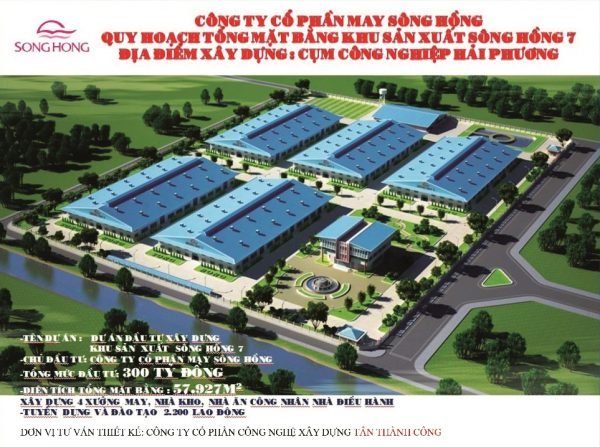
\includegraphics[width=104mm,height=77.5mm]{../../public/project-assets/songhong7.jpg}};
    \fill[TTCDeepNavy,opacity=.88] (0,148) rectangle (104,160);
    \node[anchor=west,text=white,font=\fontsize{7}{8}\selectfont\bfseries]
      at (4,154) {实景效果 • 南定省海后县};
  \end{scope}
  \draw[TTCBorder,rounded corners=4pt,line width=.7pt] (0,148) rectangle (104,220);

  \fill[TTCDeepNavy,rounded corners=4pt] (108,148) rectangle (186,220);
  \node[anchor=north west,text=TTCCyan,font=\fontsize{7.2}{8.5}\selectfont\bfseries]
    at (114,214) {项目核心参数};
  \node[anchor=north west,text=white,font=\fontsize{15}{16}\selectfont\bfseries]
    at (114,205) {68,000 m$^2$};
  \node[anchor=north west,text=white!75!gray,font=\fontsize{6.5}{8}\selectfont]
    at (114,190) {总建筑面积};
  \draw[white!25!gray] (114,183) -- (180,183);
  \node[anchor=north west,text width=62mm,align=left,text=white,
        font=\fontsize{7.2}{9}\selectfont]
    at (114,178) {\textbf{建筑形式：} 双层重型钢结构工业厂房\\[1mm]
                  \textbf{楼面荷载：} 1,200 kg/m$^2$ (重载设计)\\[1mm]
                  \textbf{建设工期：} 180 天完工\\[1mm]
                  \textbf{承包范围：} 方案深化设计与施工总承包};

  % 结构剖面原理图
  \node[anchor=west,text=TTCBlue,font=\fontsize{8}{9.5}\selectfont\bfseries]
    at (0,140) {结构受力与减振剖面原理图};
  \fill[TTCLightBlue,rounded corners=4pt] (0,53) rectangle (186,134);
  \draw[TTCBorder,rounded corners=4pt,line width=.7pt] (0,53) rectangle (186,134);

  % 框架示意
  \draw[TTCBlue,line width=1.2pt] (10,67) -- (132,67);
  \draw[TTCBlue,line width=2pt] (12,94) -- (130,94);
  \draw[TTCBlue,line width=1.2pt] (12,122) -- (71,130) -- (130,122);
  \foreach \x in {16,44,72,100,128}{
    \draw[TTCBlue,line width=1.2pt] (\x,67) -- (\x,122);
  }
  \foreach \x in {26,54,82,110}{
    \fill[white] (\x,98) rectangle +(15,7);
    \draw[TTCBorder] (\x,98) rectangle +(15,7);
    \draw[-{Latex[length=2mm]},TTCRed,line width=.8pt] (\x+7.5,108) -- (\x+7.5,96);
  }
  \node[anchor=west,text=TTCRed,font=\fontsize{6.5}{8}\selectfont\bfseries]
    at (16,112) {二层密集成组设备动荷载};
  \draw[TTCCyan,line width=1.2pt,dashed] (17,87) -- (127,87);
  \node[anchor=west,text=TTCCyan,font=\fontsize{6.3}{7.5}\selectfont\bfseries]
    at (19,82) {楼板下部预留机电/暖通管道夹层};
  \draw[<->,>=Latex,TTCBlue,line width=.8pt] (16,60) -- (128,60);
  \node[fill=TTCLightBlue,text=TTCBlue,font=\fontsize{6.5}{8}\selectfont\bfseries]
    at (72,60) {双层开阔高效生产作业面};

  % 右侧设计要点
  \draw[TTCBorder] (138,60) -- (138,127);
  \node[anchor=north west,text=TTCBlue,font=\fontsize{7.2}{8.5}\selectfont\bfseries]
    at (145,124) {三大关键设计决策};
  \node[anchor=north west,text width=34mm,align=left,text=TTCTextDark,
        font=\fontsize{6.7}{8.3}\selectfont]
    at (145,114) {\textbf{01 • 组合楼板}\newline
                  压型钢板组合楼板浇筑混凝土，承载 1.2 吨/m$^2$。};
  \node[anchor=north west,text width=34mm,align=left,text=TTCTextDark,
        font=\fontsize{6.7}{8.3}\selectfont]
    at (145,92) {\textbf{02 • 减振控制}\newline
                  合理布置次梁与刚性支撑，有效吸收设备微振动。};
  \node[anchor=north west,text width=34mm,align=left,text=TTCTextDark,
        font=\fontsize{6.7}{8.3}\selectfont]
    at (145,70) {\textbf{03 • 综合管线}\newline
                  预留机电与暖通管线空间，保证一层净高与美观。};

  % 总结卡片
  \fill[white,rounded corners=3pt] (0,9) rectangle (58,45);
  \draw[TTCBorder,rounded corners=3pt] (0,9) rectangle (58,45);
  \node[anchor=north west,text=TTCRed,font=\fontsize{8}{9}\selectfont\bfseries]
    at (5,39) {01 • 超重荷载};
  \node[anchor=north west,text width=48mm,text=TTCTextDark,font=\fontsize{6.8}{8.4}\selectfont]
    at (5,30) {二层高标准承载设计，满足成套自动化缝纫机组安全运转。};

  \fill[white,rounded corners=3pt] (64,9) rectangle (122,45);
  \draw[TTCBorder,rounded corners=3pt] (64,9) rectangle (122,45);
  \node[anchor=north west,text=TTCBlue,font=\fontsize{8}{9}\selectfont\bfseries]
    at (69,39) {02 • 专业协同};
  \node[anchor=north west,text width=48mm,text=TTCTextDark,font=\fontsize{6.8}{8.4}\selectfont]
    at (69,30) {结构预留洞口与MEP管线在BIM中100\%对齐，零现场开凿。};

  \fill[white,rounded corners=3pt] (128,9) rectangle (186,45);
  \draw[TTCBorder,rounded corners=3pt] (128,9) rectangle (186,45);
  \node[anchor=north west,text=TTCBlue,font=\fontsize{8}{9}\selectfont\bfseries]
    at (133,39) {03 • 高效节拍};
  \node[anchor=north west,text width=48mm,text=TTCTextDark,font=\fontsize{6.8}{8.4}\selectfont]
    at (133,30) {钢构安装、楼板浇筑与机电安装流水作业，180天竣工。};

  \fill[TTCDeepNavy,rounded corners=2pt] (0,0) rectangle (186,6);
\end{tikzpicture}
\end{minipage}
\newpage

% ============================================================
% TRANG 24: PROCESS CASE -- TỔ HỢP JAPFA COMFEED
% ============================================================
\noindent\mbox{}\par\vspace{-\baselineskip}
\casepagebars{工业工艺装置 • JAPFA COMFEED 饲料厂}{第24页}

\begin{minipage}[t][246mm]{\textwidth}
\secbrand{经典工程案例 03: JAPFA COMFEED 饲料生产基地}{Process-industry case • High-rise silo • Dynamic-load and dust control}

\noindent
\begin{tikzpicture}[x=1mm,y=1mm]
  \path[use as bounding box] (0,0) rectangle (186,220);

  % 照片与指标
  \begin{scope}
    \clip[rounded corners=4pt] (0,151) rectangle (68,219);
    \node[inner sep=0pt] at (34,185)
      {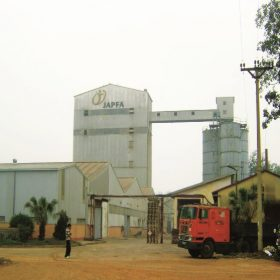
\includegraphics[width=68mm,height=68mm]{../../public/project-assets/japfa.jpg}};
    \fill[TTCDeepNavy,opacity=.9] (0,151) rectangle (68,162);
    \node[anchor=west,text=white,font=\fontsize{7}{8}\selectfont\bfseries]
      at (4,156.5) {实景 • JAPFA COMFEED};
  \end{scope}
  \draw[TTCBorder,rounded corners=4pt,line width=.7pt] (0,151) rectangle (68,219);

  \fill[TTCLightBlue,rounded corners=4pt] (72,151) rectangle (186,219);
  \draw[TTCBorder,rounded corners=4pt,line width=.7pt] (72,151) rectangle (186,219);
  \node[anchor=west,text=TTCBlue,font=\fontsize{8}{9.5}\selectfont\bfseries]
    at (78,211) {永福省 / 太平省 基地项目};
  \draw[TTCBorder] (129,158) -- (129,204);
  \draw[TTCBorder] (78,181) -- (180,181);
  \node[align=center,text width=45mm] at (103.5,193) {
    {\fontsize{12}{13}\selectfont\bfseries\color{TTCRed}50,000 m$^2$}\\[-.5mm]
    {\fontsize{6.2}{7.4}\selectfont\color{TTCTextMuted}规划总用地}};
  \node[align=center,text width=45mm] at (154.5,193) {
    {\fontsize{12}{13}\selectfont\bfseries\color{TTCBlue}筒仓高 45米}\\[-.5mm]
    {\fontsize{6.2}{7.4}\selectfont\color{TTCTextMuted}高耸塔架群}};
  \node[align=center,text width=45mm] at (103.5,169) {
    {\fontsize{12}{13}\selectfont\bfseries\color{TTCBlue}2,800 吨}\\[-.5mm]
    {\fontsize{6.2}{7.4}\selectfont\color{TTCTextMuted}PEB 钢结构总量}};
  \node[align=center,text width=45mm] at (154.5,169) {
    {\fontsize{12}{13}\selectfont\bfseries\color{TTCBlue}165 天}\\[-.5mm]
    {\fontsize{6.2}{7.4}\selectfont\color{TTCTextMuted}施工安装工期}};

  % 筒仓示意
  \node[anchor=west,text=TTCBlue,font=\fontsize{8}{9.5}\selectfont\bfseries]
    at (0,143) {工程攻坚故事 • 从深桩动荷载基础到45米高空筒仓};
  \fill[TTCLightBlue,rounded corners=4pt] (0,56) rectangle (54,137);
  \draw[TTCBorder,rounded corners=4pt,line width=.7pt] (0,56) rectangle (54,137);

  \fill[TTCBlue!10!white] (19,69) rectangle (42,123);
  \draw[TTCBlue,line width=1.1pt] (19,69) rectangle (42,123);
  \foreach \y in {80,91,102,113}{\draw[TTCBorder] (19,\y) -- (42,\y);}
  \draw[TTCBlue,line width=1.1pt] (16,69) -- (45,69);
  \fill[TTCDeepNavy] (12,62) rectangle (49,69);
  \draw[<->,>=Latex,TTCRed,line width=.9pt] (9,69) -- (9,123);
  \node[rotate=90,text=TTCRed,font=\fontsize{9}{10}\selectfont\bfseries]
    at (4,96) {45 米高度};
  \node[text=TTCBlue,font=\fontsize{6.5}{7.5}\selectfont\bfseries]
    at (30.5,129) {筒仓塔架群};
  \node[text=white,font=\fontsize{6.2}{7.2}\selectfont\bfseries]
    at (30.5,65.5) {D800 灌注桩};

  % 三大应对措施
  \fill[white,rounded corners=3pt] (60,108) rectangle (186,137);
  \draw[TTCBorder,rounded corners=3pt] (60,108) rectangle (186,137);
  \fill[TTCRed] (60,108) rectangle (63,137);
  \node[anchor=north west,text=TTCBlue,font=\fontsize{8}{9}\selectfont\bfseries]
    at (69,132) {01 • 粉碎机组动荷载减振};
  \node[anchor=north west,text width=108mm,text=TTCTextDark,font=\fontsize{6.9}{8.4}\selectfont]
    at (69,122) {采用 D800 深孔灌注桩基础与阻尼隔振垫层，精准吸收重型旋转机械动力冲击波。};

  \fill[white,rounded corners=3pt] (60,76) rectangle (186,105);
  \draw[TTCBorder,rounded corners=3pt] (60,76) rectangle (186,105);
  \fill[TTCBlue] (60,76) rectangle (63,105);
  \node[anchor=north west,text=TTCBlue,font=\fontsize{8}{9}\selectfont\bfseries]
    at (69,100) {02 • 45米高空分段精准吊装};
  \node[anchor=north west,text width=108mm,text=TTCTextDark,font=\fontsize{6.9}{8.4}\selectfont]
    at (69,90) {塔架结构分段预拼装，激光测距仪全程监控垂直度与法兰平整度，误差控制在 2mm 内。};

  \fill[white,rounded corners=3pt] (60,44) rectangle (186,73);
  \draw[TTCBorder,rounded corners=3pt] (60,44) rectangle (186,73);
  \fill[TTCBlue] (60,44) rectangle (63,73);
  \node[anchor=north west,text=TTCBlue,font=\fontsize{8}{9}\selectfont\bfseries]
    at (69,68) {03 • 粉尘防爆与消防安全};
  \node[anchor=north west,text width=108mm,text=TTCTextDark,font=\fontsize{6.9}{8.4}\selectfont]
    at (69,58) {全面集成旋风除尘、负压通风及泄爆阀门装置，达到粮食饲料行业严苛的防爆安全标准。};

  % 实施范围
  \fill[TTCDeepNavy,rounded corners=4pt] (0,0) rectangle (186,35);
  \node[anchor=west,text=TTCCyan,font=\fontsize{6.5}{8}\selectfont\bfseries]
    at (7,28) {TTC 实施范围};
  \foreach \x in {46.5,93,139.5}{\draw[white!25!gray] (\x,6) -- (\x,25);}
  \node[align=center,text width=39mm,text=white,font=\fontsize{7.2}{8.5}\selectfont\bfseries]
    at (23.25,15) {深桩基础工程\\[-.5mm]{\fontsize{5.8}{7}\selectfont\color{white!70!gray}静载+动载复合验算}};
  \node[align=center,text width=39mm,text=white,font=\fontsize{7.2}{8.5}\selectfont\bfseries]
    at (69.75,15) {PEB 钢结构制造\\[-.5mm]{\fontsize{5.8}{7}\selectfont\color{white!70!gray}高耸塔架精密加工}};
  \node[align=center,text width=39mm,text=white,font=\fontsize{7.2}{8.5}\selectfont\bfseries]
    at (116.25,15) {筒仓高空安装\\[-.5mm]{\fontsize{5.8}{7}\selectfont\color{white!70!gray}高精度垂直度控制}};
  \node[align=center,text width=39mm,text=white,font=\fontsize{7.2}{8.5}\selectfont\bfseries]
    at (162.75,15) {工艺配套系统\\[-.5mm]{\fontsize{5.8}{7}\selectfont\color{white!70!gray}防爆 • 除尘 • 变配电}};
\end{tikzpicture}
\end{minipage}
\newpage

% ============================================================
% TRANG 25: CLEANROOM CASE -- DAEYUN ST VINA
% ============================================================
\noindent\mbox{}\par\vspace{-\baselineskip}
\casepagebars{高等级无尘车间 • 大润科技 DAEYUN ST VINA}{第25页}

\begin{minipage}[t][246mm]{\textwidth}
\secbrand{经典工程案例 04: 大润科技 DAEYUN ST VINA 厂房}{Integrated cleanroom systems • KCN Bá Thiện 2, Vĩnh Phúc}

\noindent
\begin{tikzpicture}[x=1mm,y=1mm]
  \path[use as bounding box] (0,0) rectangle (186,220);

  % 实景
  \begin{scope}
    \clip[rounded corners=4pt] (0,157) rectangle (118,219);
    \node[inner sep=0pt] at (59,188)
      {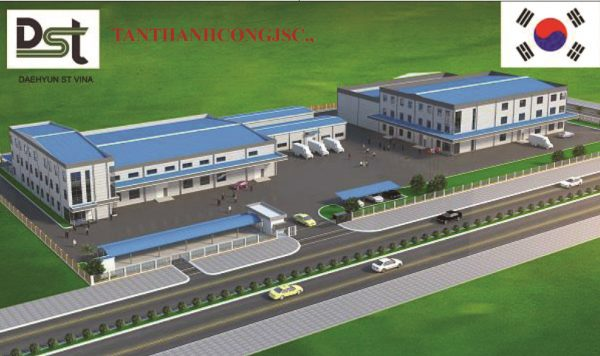
\includegraphics[width=118mm]{../../public/project-assets/daeyun.jpg}};
    \fill[TTCDeepNavy,opacity=.88] (0,157) rectangle (118,168);
    \node[anchor=west,text=white,font=\fontsize{7}{8}\selectfont\bfseries]
      at (4,162.5) {工程实景 • 永福省霸善二期工业区};
  \end{scope}
  \draw[TTCBorder,rounded corners=4pt,line width=.7pt] (0,157) rectangle (118,219);

  \fill[TTCDeepNavy,rounded corners=4pt] (122,157) rectangle (186,219);
  \node[anchor=north west,text=TTCCyan,font=\fontsize{7.2}{8.5}\selectfont\bfseries]
    at (128,213) {工程基本信息};
  \node[anchor=north west,text=white,font=\fontsize{13}{14}\selectfont\bfseries]
    at (128,203) {20,000 m$^2$};
  \node[anchor=north west,text=white!70!gray,font=\fontsize{6}{7.2}\selectfont]
    at (128,190) {洁净车间面积};
  \draw[white!25!gray] (128,184) -- (180,184);
  \node[anchor=north west,text width=48mm,align=left,text=white,
        font=\fontsize{6.8}{8.4}\selectfont]
    at (128,180) {\textbf{洁净等级：} Class 10,000\\
                  \textbf{特殊要求：} ESD 防静电\\
                  \textbf{建设工期：} 140 天};

  % 系统图
  \node[anchor=west,text=TTCBlue,font=\fontsize{8}{9.5}\selectfont\bfseries]
    at (0,149) {四大子系统高度集成 • 确保洁净度稳定达标};
  \fill[TTCLightBlue,rounded corners=4pt] (0,57) rectangle (186,143);
  \draw[TTCBorder,rounded corners=4pt,line width=.7pt] (0,57) rectangle (186,143);

  % 核心区
  \fill[TTCDeepNavy,rounded corners=4pt] (68,88) rectangle (118,116);
  \node[align=center,text=white,text width=42mm,font=\fontsize{8}{9.5}\selectfont\bfseries]
    at (93,102) {核心洁净生产区\\[-.5mm]
    {\fontsize{6}{7.2}\selectfont\color{white!70!gray}恒温恒湿 • 密闭 • 防静电}};

  % 四个外围模块
  \fill[white,rounded corners=3pt] (7,108) rectangle (58,136);
  \draw[TTCBorder,rounded corners=3pt] (7,108) rectangle (58,136);
  \node[anchor=north west,text=TTCBlue,font=\fontsize{7.5}{8.5}\selectfont\bfseries]
    at (12,131) {01 • 洁净密闭围护};
  \node[anchor=north west,text width=41mm,text=TTCTextDark,font=\fontsize{6.4}{7.8}\selectfont]
    at (12,121) {高精度气密彩钢夹芯板与吊顶系统，确保正压梯度与无尘环境。};

  \fill[white,rounded corners=3pt] (128,108) rectangle (179,136);
  \draw[TTCBorder,rounded corners=3pt] (128,108) rectangle (179,136);
  \node[anchor=north west,text=TTCBlue,font=\fontsize{7.5}{8.5}\selectfont\bfseries]
    at (133,131) {02 • AHU / HEPA 空调};
  \node[anchor=north west,text width=41mm,text=TTCTextDark,font=\fontsize{6.4}{7.8}\selectfont]
    at (133,121) {初中高效三级过滤送风与高效回风系统，精确控制换气次数。};

  \fill[white,rounded corners=3pt] (7,64) rectangle (58,92);
  \draw[TTCBorder,rounded corners=3pt] (7,64) rectangle (58,92);
  \node[anchor=north west,text=TTCRed,font=\fontsize{7.5}{8.5}\selectfont\bfseries]
    at (12,87) {03 • 精密温湿度控制};
  \node[anchor=north west,text width=41mm,text=TTCTextDark,font=\fontsize{6.4}{7.8}\selectfont]
    at (12,77) {温度 $\pm1^\circ$C、湿度 $\pm5\%$ 恒定控制，满足精密贴片工艺。};

  \fill[white,rounded corners=3pt] (128,64) rectangle (179,92);
  \draw[TTCBorder,rounded corners=3pt] (128,64) rectangle (179,92);
  \node[anchor=north west,text=TTCBlue,font=\fontsize{7.5}{8.5}\selectfont\bfseries]
    at (133,87) {04 • ESD 防静电地坪};
  \node[anchor=north west,text width=41mm,text=TTCTextDark,font=\fontsize{6.4}{7.8}\selectfont]
    at (133,77) {导静电 PVC 地板与接地铜网系统，彻底杜绝静电对元器件损伤。};

  \draw[-{Latex[length=2mm]},TTCCyan,line width=.9pt] (58,122) -- (68,108);
  \draw[-{Latex[length=2mm]},TTCCyan,line width=.9pt] (128,122) -- (118,108);
  \draw[-{Latex[length=2mm]},TTCCyan,line width=.9pt] (58,78) -- (68,94);
  \draw[-{Latex[length=2mm]},TTCCyan,line width=.9pt] (128,78) -- (118,94);

  % 总结
  \fill[white,rounded corners=3pt] (0,10) rectangle (58,48);
  \draw[TTCBorder,rounded corners=3pt] (0,10) rectangle (58,48);
  \node[align=center,text width=48mm] at (29,29) {
    {\fontsize{10}{11}\selectfont\bfseries\color{TTCRed}Class 10,000}\\[-.5mm]
    {\fontsize{6.4}{7.6}\selectfont\color{TTCTextMuted}万级无尘车间标准}};

  \fill[white,rounded corners=3pt] (64,10) rectangle (122,48);
  \draw[TTCBorder,rounded corners=3pt] (64,10) rectangle (122,48);
  \node[align=center,text width=48mm] at (93,29) {
    {\fontsize{10}{11}\selectfont\bfseries\color{TTCBlue}ESD 防静电}\\[-.5mm]
    {\fontsize{6.4}{7.6}\selectfont\color{TTCTextMuted}电子元器件全方位保护}};

  \fill[white,rounded corners=3pt] (128,10) rectangle (186,48);
  \draw[TTCBorder,rounded corners=3pt] (128,10) rectangle (186,48);
  \node[align=center,text width=48mm] at (157,29) {
    {\fontsize{10}{11}\selectfont\bfseries\color{TTCBlue}140 天完工}\\[-.5mm]
    {\fontsize{6.4}{7.6}\selectfont\color{TTCTextMuted}高效准时履约交付}};

  \fill[TTCDeepNavy,rounded corners=2pt] (0,0) rectangle (186,6);
\end{tikzpicture}
\end{minipage}
\newpage

% ============================================================
% TRANG 26: QUALITY DELIVERY -- SUMIDENSO VINA
% ============================================================
\noindent\mbox{}\par\vspace{-\baselineskip}
\casepagebars{高品质履约交付 • 住友电工 SUMIDENSO}{第26页}

\begin{minipage}[t][246mm]{\textwidth}
\secbrand{经典工程案例 05: 住友电工 SUMIDENSO 汽车线束工厂}{Quality-led delivery • Automotive wire harness plant • KCN Sông Hậu, Hậu Giang}

\noindent
\begin{tikzpicture}[x=1mm,y=1mm]
  \path[use as bounding box] (0,0) rectangle (186,220);

  % 厂区照片与概况
  \begin{scope}
    \clip[rounded corners=4pt] (0,155) rectangle (64,219);
    \node[inner sep=0pt] at (32,187)
      {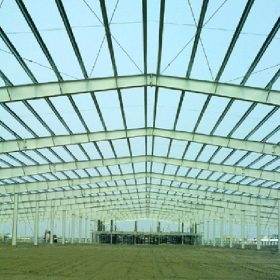
\includegraphics[width=64mm,height=64mm]{../../public/project-assets/sumidenso.jpg}};
    \fill[TTCDeepNavy,opacity=.88] (0,155) rectangle (64,166);
    \node[anchor=west,text=white,font=\fontsize{6.8}{8}\selectfont\bfseries]
      at (4,160.5) {厂区厂房实景};
  \end{scope}
  \draw[TTCBorder,rounded corners=4pt,line width=.7pt] (0,155) rectangle (64,219);

  \fill[TTCLightBlue,rounded corners=4pt] (68,155) rectangle (186,219);
  \draw[TTCBorder,rounded corners=4pt,line width=.7pt] (68,155) rectangle (186,219);
  \node[anchor=north west,text=TTCBlue,font=\fontsize{8}{9.5}\selectfont\bfseries]
    at (75,212) {项目档案概览};
  \node[anchor=north west,text width=48mm,text=TTCTextDark,font=\fontsize{7.1}{8.8}\selectfont]
    at (75,201) {\textbf{投资业主：} 住友电工 (Sumitomo)\\
                  \textbf{建筑面积：} 15,015 m$^2$\\
                  \textbf{建设工期：} 150 天};
  \draw[TTCBorder] (129,161) -- (129,208);
  \node[anchor=north west,text=TTCBlue,font=\fontsize{8}{9.5}\selectfont\bfseries]
    at (136,212) {重点交付保障};
  \node[anchor=north west,text width=43mm,text=TTCTextDark,font=\fontsize{6.9}{8.5}\selectfont]
    at (136,201) {\textbullet\quad 快速响应式自动喷淋系统\\[1mm]
                  \textbullet\quad 达标工业污水处理站\\[1mm]
                  \textbullet\quad 日企严苛的验收归档管理};

  % 四道质量关口
  \node[anchor=west,text=TTCBlue,font=\fontsize{8}{9.5}\selectfont\bfseries]
    at (0,147) {日系精细化 4 级质量控制关口};
  \fill[white,rounded corners=4pt] (0,88) rectangle (186,141);
  \draw[TTCBorder,rounded corners=4pt,line width=.7pt] (0,88) rectangle (186,141);
  \draw[TTCBlue,line width=.8pt] (23,122) -- (163,122);

  \foreach \x/\n in {23/01,69/02,117/03,163/04}{
    \fill[white] (\x,122) circle (6mm);
    \draw[TTCBlue,line width=.9pt] (\x,122) circle (6mm);
    \node[text=TTCBlue,font=\fontsize{7}{8}\selectfont\bfseries] at (\x,122) {\n};
  }
  \fill[TTCRed] (23,122) circle (3.2mm);
  \node[text=white,font=\fontsize{6.2}{7}\selectfont\bfseries] at (23,122) {01};

  \node[align=center,text width=38mm] at (23,101) {
    {\fontsize{7.3}{8.5}\selectfont\bfseries\color{TTCBlue}进场材料检验}\\[-.3mm]
    {\fontsize{5.9}{7.1}\selectfont\color{TTCTextMuted}CO/CQ • 封样比对 • 批次溯源}};
  \node[align=center,text width=38mm] at (69,101) {
    {\fontsize{7.3}{8.5}\selectfont\bfseries\color{TTCBlue}过程 ITP 检验}\\[-.3mm]
    {\fontsize{5.9}{7.1}\selectfont\color{TTCTextMuted}见证点 • 停止点 • 逐项验收}};
  \node[align=center,text width=38mm] at (117,101) {
    {\fontsize{7.3}{8.5}\selectfont\bfseries\color{TTCBlue}系统联合调试}\\[-.3mm]
    {\fontsize{5.9}{7.1}\selectfont\color{TTCTextMuted}消防联动 • 污水达标 • 试运转}};
  \node[align=center,text width=38mm] at (163,101) {
    {\fontsize{7.3}{8.5}\selectfont\bfseries\color{TTCBlue}档案移交培训}\\[-.3mm]
    {\fontsize{5.9}{7.1}\selectfont\color{TTCTextMuted}竣工图 • 操作手册 • 维保培训}};

  % 表格
  \node[anchor=west,text=TTCBlue,font=\fontsize{8}{9.5}\selectfont\bfseries]
    at (0,80) {技术需求、质量控制点与交付凭证对照表};
  \fill[TTCDeepNavy,rounded corners=3pt] (0,62) rectangle (186,75);
  \node[anchor=west,text=white,font=\fontsize{6.5}{7.8}\selectfont\bfseries] at (6,68.5) {工程分项};
  \node[anchor=west,text=white,font=\fontsize{6.5}{7.8}\selectfont\bfseries] at (55,68.5) {关键控制节点};
  \node[anchor=west,text=white,font=\fontsize{6.5}{7.8}\selectfont\bfseries] at (126,68.5) {移交凭据与报告};

  \fill[TTCLightBlue] (0,47) rectangle (186,62);
  \fill[white] (0,32) rectangle (186,47);
  \fill[TTCLightBlue] (0,17) rectangle (186,32);
  \draw[TTCBorder] (49,17) -- (49,75);
  \draw[TTCBorder] (120,17) -- (120,75);
  \foreach \y in {17,32,47,62}{\draw[TTCBorder] (0,\y) -- (186,\y);}
  \node[anchor=west,text=TTCBlue,font=\fontsize{6.6}{8}\selectfont\bfseries] at (6,54.5) {消防喷淋系统};
  \node[anchor=west,text=TTCTextDark,font=\fontsize{6.4}{7.8}\selectfont] at (55,54.5) {压力试验 • 水流量 • 联动报警};
  \node[anchor=west,text=TTCTextDark,font=\fontsize{6.4}{7.8}\selectfont] at (126,54.5) {消防局官方验收合格批文};
  \node[anchor=west,text=TTCBlue,font=\fontsize{6.6}{8}\selectfont\bfseries] at (6,39.5) {污水处理系统};
  \node[anchor=west,text=TTCTextDark,font=\fontsize{6.4}{7.8}\selectfont] at (55,39.5) {试运行出水水质检测};
  \node[anchor=west,text=TTCTextDark,font=\fontsize{6.4}{7.8}\selectfont] at (126,39.5) {QCVN 40 A级第三方水质报告};
  \node[anchor=west,text=TTCBlue,font=\fontsize{6.6}{8}\selectfont\bfseries] at (6,24.5) {装饰装修工程};
  \node[anchor=west,text=TTCTextDark,font=\fontsize{6.4}{7.8}\selectfont] at (55,24.5) {平整度 • 收口细节 • 深度清洁};
  \node[anchor=west,text=TTCTextDark,font=\fontsize{6.4}{7.8}\selectfont] at (126,24.5) {Punch List 缺陷清零签署单};

  \fill[TTCDeepNavy,rounded corners=3pt] (0,0) rectangle (186,11);
  \node[anchor=west,text=white,font=\fontsize{7}{8.5}\selectfont\bfseries]
    at (7,5.5) {15,015 m$^2$};
  \node[text=white!35!gray] at (49,5.5) {|};
  \node[anchor=west,text=white,font=\fontsize{7}{8.5}\selectfont\bfseries]
    at (57,5.5) {150 天交付};
  \node[text=white!35!gray] at (95,5.5) {|};
  \node[anchor=west,text=white,font=\fontsize{7}{8.5}\selectfont\bfseries]
    at (103,5.5) {消防与污水处理系统一次性通过日方验收};
\end{tikzpicture}
\end{minipage}
\newpage

% ============================================================
% TRANG 27: PROJECT SPOTLIGHT -- XƯỞNG SẢN XUẤT FOXCONN
% ============================================================
\noindent\mbox{}\par\vspace{-\baselineskip}
\casepagebars{高精密电子厂房 • 富士康 FOXCONN}{第27页}

\begin{minipage}[t][246mm]{\textwidth}
\secbrand{经典工程案例 06: 富士康 FOXCONN 生产车间}{Electronics manufacturing facility • KCN Quế Võ, Bắc Ninh}

\noindent
\begin{tikzpicture}[x=1mm,y=1mm]
  \path[use as bounding box] (0,0) rectangle (186,220);

  % 实景
  \begin{scope}
    \clip[rounded corners=4pt] (0,151) rectangle (186,219);
    \node[inner sep=0pt] at (93,185)
      {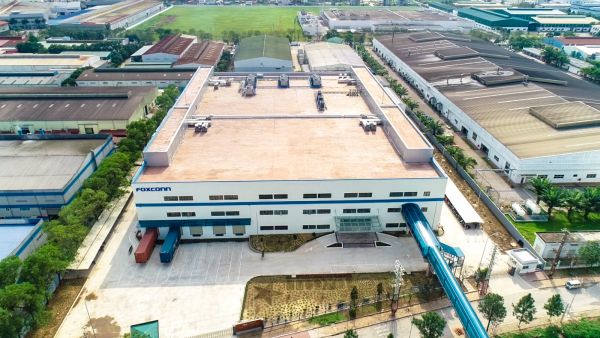
\includegraphics[width=186mm]{../../public/project-assets/foxcon.png}};
    \fill[TTCDeepNavy,opacity=.9] (0,151) rectangle (78,168);
    \node[anchor=west,text=white,font=\fontsize{7}{8}\selectfont\bfseries]
      at (5,159.5) {工程实景 • 北宁省桂武工业区};
    \fill[TTCDeepNavy,opacity=.92] (127,151) rectangle (186,219);
    \node[anchor=north west,text=TTCCyan,font=\fontsize{6.8}{8}\selectfont\bfseries]
      at (133,212) {项目档案概览};
    \node[anchor=north west,text=white,font=\fontsize{14}{15}\selectfont\bfseries]
      at (133,201) {12,000 m$^2$};
    \node[anchor=north west,text=white!70!gray,font=\fontsize{6}{7.2}\selectfont]
      at (133,187) {车间建筑面积};
    \draw[white!25!gray] (133,181) -- (180,181);
    \node[anchor=north west,text width=43mm,text=white,font=\fontsize{6.5}{8}\selectfont]
      at (133,177) {\textbf{投资业主：} 富士康 (Foxconn)\\
                    \textbf{企业背景：} 中国台湾知名跨国集团\\
                    \textbf{承包范围：} 钢结构制造与高空安装};
  \end{scope}
  \draw[TTCBorder,rounded corners=4pt,line width=.7pt] (0,151) rectangle (186,219);

  % 施工流
  \node[anchor=west,text=TTCBlue,font=\fontsize{8}{9.5}\selectfont\bfseries]
    at (0,143) {安装前锁定关键技术接口 • 分区流水高效推进};
  \fill[TTCLightBlue,rounded corners=4pt] (0,68) rectangle (186,137);
  \draw[TTCBorder,rounded corners=4pt,line width=.7pt] (0,68) rectangle (186,137);

  \foreach \xa/\xb in {4/43,50/89,96/135,142/182}{
    \fill[white,rounded corners=3pt] (\xa,74) rectangle (\xb,132);
    \draw[TTCBorder,rounded corners=3pt,line width=.65pt] (\xa,74) rectangle (\xb,132);
    \draw[TTCBlue,line width=1.2pt] ({\xa+4},128) -- ({\xb-4},128);
  }
  \foreach \xa/\xb in {43/50,89/96,135/142}{
    \draw[-{Latex[length=2mm]},TTCBlue!65!white,line width=.8pt]
      ({\xa+1},103) -- ({\xb-1},103);
  }

  \fill[TTCRed] (10,122) circle (3.5mm);
  \node[text=white,font=\fontsize{6}{7}\selectfont\bfseries] at (10,122) {01};
  \node[anchor=north west,text width=29mm,align=left,text=TTCBlue,
        font=\fontsize{7.2}{8.5}\selectfont\bfseries]
    at (9,115) {设计模型\\接口锁定};
  \node[anchor=north west,text width=29mm,align=left,text=TTCTextMuted,
        font=\fontsize{6.1}{7.4}\selectfont]
    at (9,96) {锁定轴线标高及钢结构与MEP接口。};

  \fill[TTCBlue] (56,122) circle (3.5mm);
  \node[text=white,font=\fontsize{6}{7}\selectfont\bfseries] at (56,122) {02};
  \node[anchor=north west,text width=29mm,align=left,text=TTCBlue,
        font=\fontsize{7.2}{8.5}\selectfont\bfseries]
    at (55,115) {工厂预制\\精密加工};
  \node[anchor=north west,text width=29mm,align=left,text=TTCTextMuted,
        font=\fontsize{6.1}{7.4}\selectfont]
    at (55,96) {数控下料与驻厂QC严控构件精度。};

  \fill[TTCBlue] (102,122) circle (3.5mm);
  \node[text=white,font=\fontsize{6}{7}\selectfont\bfseries] at (102,122) {03};
  \node[anchor=north west,text width=29mm,align=left,text=TTCBlue,
        font=\fontsize{7.2}{8.5}\selectfont\bfseries]
    at (101,115) {分区流水\\安全吊装};
  \node[anchor=north west,text width=29mm,align=left,text=TTCTextMuted,
        font=\fontsize{6.1}{7.4}\selectfont]
    at (101,96) {形成稳定空间刚度单元，流水推进。};

  \fill[TTCBlue] (148,122) circle (3.5mm);
  \node[text=white,font=\fontsize{6}{7}\selectfont\bfseries] at (148,122) {04};
  \node[anchor=north west,text width=29mm,align=left,text=TTCBlue,
        font=\fontsize{7.2}{8.5}\selectfont\bfseries]
    at (147,115) {工序交接\\验收放行};
  \node[anchor=north west,text width=29mm,align=left,text=TTCTextMuted,
        font=\fontsize{6.1}{7.4}\selectfont]
    at (147,96) {几何尺寸与高强螺栓终拧100\%复验。};

  % 两大核心要点
  \fill[white,rounded corners=4pt] (0,19) rectangle (90,60);
  \draw[TTCBorder,rounded corners=4pt] (0,19) rectangle (90,60);
  \node[anchor=north west,text=TTCRed,font=\fontsize{8}{9}\selectfont\bfseries]
    at (6,54) {项目核心难点};
  \node[anchor=north west,text width=77mm,align=left,text=TTCTextDark,
        font=\fontsize{6.9}{8.5}\selectfont]
    at (6,44) {电子厂房空间开阔、机电管网密集，且要求施工吊装绝不能干扰毗邻既有车间的正常生产运作。};

  \fill[TTCLightBlue,rounded corners=4pt] (96,19) rectangle (186,60);
  \draw[TTCBorder,rounded corners=4pt] (96,19) rectangle (186,60);
  \node[anchor=north west,text=TTCBlue,font=\fontsize{8}{9.5}\selectfont\bfseries]
    at (102,54) {TTC 实施策略};
  \node[anchor=north west,text width=77mm,align=left,text=TTCTextDark,
        font=\fontsize{6.9}{8.5}\selectfont]
    at (102,44) {采用模块化分区施工方案，后方基地精确预制，现场夜间错峰吊装并逐段移交安装作业面。};

  \fill[TTCDeepNavy,rounded corners=3pt] (0,0) rectangle (186,12);
  \node[anchor=west,text=TTCCyan,font=\fontsize{6.2}{7.4}\selectfont\bfseries]
    at (7,6) {实施原则};
  \draw[white!28!gray] (47,3) -- (47,9);
  \node[anchor=west,text=white,font=\fontsize{7}{8.5}\selectfont\bfseries]
    at (54,6) {锁定技术接口 → 分区流水作业 → 严密工序验收};
\end{tikzpicture}
\end{minipage}
\newpage

% ============================================================
% TRANG 28: CHUỖI CUNG ỨNG KIỂM SOÁT
% ============================================================
\noindent\mbox{}\par\vspace{-\baselineskip}
\casepagebars{严格受控的战略供应链体系}{第28页}

\begin{minipage}[t][246mm]{\textwidth}
\secbrand{按批次严格受控的战略供应链}{Approved sources • Material submittal • CO/CQ/MTC • Lot traceability}

\noindent
\begin{tikzpicture}[x=1mm,y=1mm]
  \path[use as bounding box] (0,0) rectangle (186,220);

  \node[anchor=west,text=TTCBlue,font=\fontsize{15}{17}\selectfont\bfseries]
    at (0,211) {全套质检文件齐备方获准进场安装};
  \node[anchor=west,text=TTCTextMuted,font=\fontsize{7.2}{8.8}\selectfont]
    at (0,201) {统一严密的物资审批报审流程，确保采购前锁定品牌源头、技术指标与替代可行性。};

  % 4道把关
  \fill[TTCDeepNavy,rounded corners=4pt] (0,79) rectangle (62,192);
  \node[anchor=west,text=TTCCyan,font=\fontsize{7}{8.3}\selectfont\bfseries]
    at (7,184) {4 级物资把关关口};
  \draw[white!18!gray] (7,178) -- (55,178);

  \foreach \y/\n/\title/\desc in {
    158/01/厂家源头报审/厂家资质 • 样品封存 • 技术规格书,
    134/02/文件闭环核验/CO-CQ • MTC质保书 • 产品型录,
    110/03/进场严格复检/批次标签 • 外观尺寸 • 试验室复验,
    88/04/安装可溯追踪/物资批次绑定施工部位与检验批单}
  {
    \fill[white,rounded corners=2pt] (7,{\y-8}) rectangle (55,{\y+8});
    \fill[TTCRed] (7,{\y-8}) rectangle (16,{\y+8});
    \node[text=white,font=\fontsize{6.2}{7}\selectfont\bfseries] at (11.5,\y) {\n};
    \node[anchor=north west,text width=34mm,text=TTCBlue,
          font=\fontsize{6.7}{7.8}\selectfont\bfseries] at (19,{\y+5}) {\title};
    \node[anchor=north west,text width=34mm,text=TTCTextMuted,
          font=\fontsize{5.6}{6.7}\selectfont] at (19,{\y-1}) {\desc};
  }

  % 材料矩阵
  \fill[white,rounded corners=4pt] (67,79) rectangle (186,192);
  \draw[TTCBorder,rounded corners=4pt,line width=.7pt] (67,79) rectangle (186,192);
  \node[anchor=west,text=TTCBlue,font=\fontsize{8}{9.4}\selectfont\bfseries]
    at (74,184) {核心材料品类 / 国际基准品牌库};
  \node[anchor=west,text=TTCTextMuted,font=\fontsize{5.8}{7}\selectfont]
    at (74,176) {实际选用品牌严格遵循各工程经业主与监理批准的材料报审表。};

  \foreach \y/\n/\name/\brands/\control in {
    157/01/钢材与围护板材/POSCO • 和发 (Hoa Phat) • 烨辉 (BlueScope)/MTC • 钢号 • 镀锌铝层,
    134/02/工业涂料与化学建材/佐敦 (Jotun) • KCC • 西卡 (Sika)/批次 • DFT漆膜 • 防火认证,
    111/03/电气与配电系统/施耐德 (Schneider) • ABB • LS Vina/型录 • 试验报告 • 原产地,
    88/04/暖通与消防系统/大金 (Daikin) • 格兰富 (Grundfos) • 泰科 (Tyco)/报审 • UL-FM 认证要求}
  {
    \fill[TTCLightBlue,rounded corners=2pt] (73,{\y-9}) rectangle (180,{\y+9});
    \node[anchor=west,text=TTCRed,font=\fontsize{6.4}{7.5}\selectfont\bfseries]
      at (78,{\y+4}) {\n};
    \node[anchor=west,text=TTCBlue,font=\fontsize{7}{8.2}\selectfont\bfseries]
      at (91,{\y+4}) {\name};
    \node[anchor=west,text=TTCTextDark,font=\fontsize{6.2}{7.3}\selectfont]
      at (91,{\y-2}) {\brands};
    \node[anchor=east,text=TTCTextMuted,font=\fontsize{5.6}{6.7}\selectfont]
      at (176,{\y-7}) {控制点：\control};
  }

  % 三大保证
  \node[anchor=west,text=TTCBlue,font=\fontsize{8}{9.4}\selectfont\bfseries]
    at (0,68) {进场安装前三大质量保证屏障};
  \foreach \xa/\xb/\n/\title/\desc in {
    0/58/01/正品正源/报审文件与厂家实际出厂来源 100\% 一致,
    64/122/02/指标达标/物理力学指标完全符合封样及工程技术规范,
    128/186/03/位批对应/每批进场材料精准对应具体构件编号与施工区域}
  {
    \fill[white,rounded corners=3pt] (\xa,25) rectangle (\xb,60);
    \draw[TTCBorder,rounded corners=3pt] (\xa,25) rectangle (\xb,60);
    \node[anchor=west,text=TTCRed,font=\fontsize{7}{8}\selectfont\bfseries]
      at ({\xa+6},52) {\n};
    \node[anchor=west,text=TTCBlue,font=\fontsize{7.4}{8.7}\selectfont\bfseries]
      at ({\xa+17},52) {\title};
    \node[anchor=north west,text width=46mm,text=TTCTextMuted,
          font=\fontsize{6.2}{7.5}\selectfont] at ({\xa+6},43) {\desc};
  }

  \fill[TTCDeepNavy,rounded corners=3pt] (0,0) rectangle (186,16);
  \node[anchor=west,text=TTCCyan,font=\fontsize{6.3}{7.5}\selectfont\bfseries]
    at (7,8) {MATERIAL ASSURANCE};
  \node[anchor=east,text=white,font=\fontsize{7.2}{8.5}\selectfont\bfseries]
    at (179,8) {核准源头 → 逐批复检 → 全程可溯安装};
\end{tikzpicture}
\end{minipage}
\newpage

% ============================================================
% TRANG 29: HỆ SINH THÁI CÔNG TRÌNH THEO NGÀNH
% ============================================================
\noindent\mbox{}\par\vspace{-\baselineskip}
\casepagebars{六大行业工业建筑生态体系}{第29页}

\begin{minipage}[t][246mm]{\textwidth}
\secbrand{六大行业定制化工程 — 一体化综合总包能力}{Representative sectors • Different operating demands • One coordinated EPC workflow}

\noindent
\begin{tikzpicture}[x=1mm,y=1mm]
  \path[use as bounding box] (0,0) rectangle (186,220);
  \node[anchor=west,text=TTCBlue,font=\fontsize{15}{17}\selectfont\bfseries]
    at (0,211) {工程设计始于对工厂工艺生产流程的深刻理解};
  \node[anchor=west,text=TTCTextMuted,font=\fontsize{7.2}{8.8}\selectfont]
    at (0,201) {每个工业领域都有其独特的运营难点；结构、机电与施工部署必须精准契合工艺安全。};

  % 行 1
  \begin{scope}
    \clip[rounded corners=3pt] (0,132) rectangle (59,190);
    \node[inner sep=0pt] at (29.5,165) {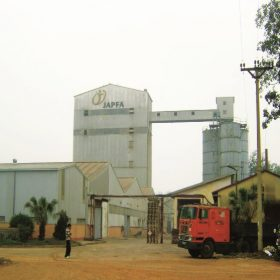
\includegraphics[width=60mm]{../../public/project-assets/japfa.jpg}};
    \fill[TTCDeepNavy,opacity=.9] (0,132) rectangle (59,151);
  \end{scope}
  \draw[TTCBorder,rounded corners=3pt] (0,132) rectangle (59,190);
  \node[anchor=west,text=white,font=\fontsize{7.5}{8.8}\selectfont\bfseries] at (5,144) {食品加工与农牧饲料};
  \node[anchor=west,text=white!75!gray,font=\fontsize{5.8}{7}\selectfont] at (5,137) {筒仓 • 工艺管网 • 洁净防尘 • 防爆};

  \begin{scope}
    \clip[rounded corners=3pt] (63.5,132) rectangle (122.5,190);
    \node[inner sep=0pt] at (93,167) {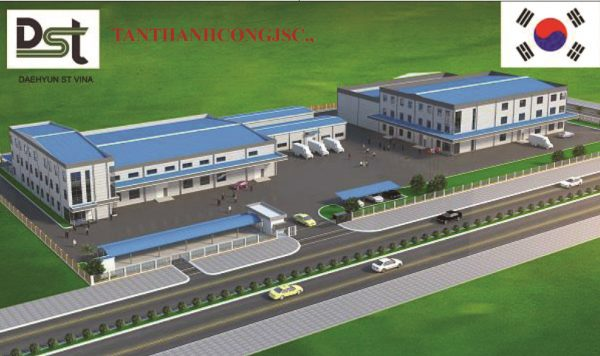
\includegraphics[height=41mm]{../../public/project-assets/daeyun.jpg}};
    \fill[TTCDeepNavy,opacity=.9] (63.5,132) rectangle (122.5,151);
  \end{scope}
  \draw[TTCBorder,rounded corners=3pt] (63.5,132) rectangle (122.5,190);
  \node[anchor=west,text=white,font=\fontsize{7.5}{8.8}\selectfont\bfseries] at (68.5,144) {半导体电子与无尘室};
  \node[anchor=west,text=white!75!gray,font=\fontsize{5.8}{7}\selectfont] at (68.5,137) {洁净空调 • ESD 防静电 • 恒温恒湿};

  \begin{scope}
    \clip[rounded corners=3pt] (127,132) rectangle (186,190);
    \node[inner sep=0pt] at (156.5,168) {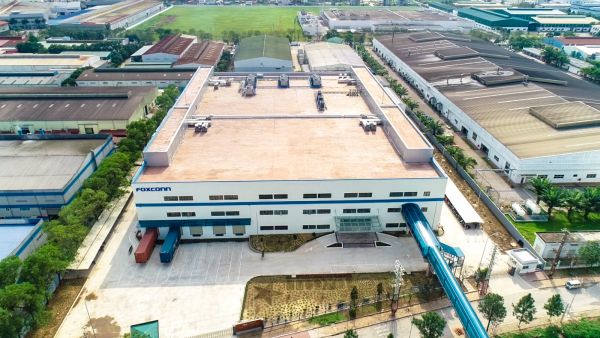
\includegraphics[height=41mm]{../../public/project-assets/foxcon.png}};
    \fill[TTCDeepNavy,opacity=.9] (127,132) rectangle (186,151);
  \end{scope}
  \draw[TTCBorder,rounded corners=3pt] (127,132) rectangle (186,190);
  \node[anchor=west,text=white,font=\fontsize{7.5}{8.8}\selectfont\bfseries] at (132,144) {精密电子组装厂房};
  \node[anchor=west,text=white!75!gray,font=\fontsize{5.8}{7}\selectfont] at (132,137) {MEP 接口锁定 • 模块化分区吊装};

  % 行 2
  \begin{scope}
    \clip[rounded corners=3pt] (0,69) rectangle (59,127);
    \node[inner sep=0pt] at (29.5,103) {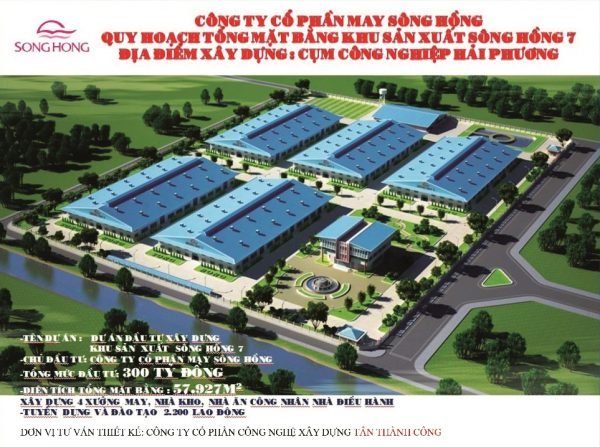
\includegraphics[height=42mm]{../../public/project-assets/songhong7.jpg}};
    \fill[TTCDeepNavy,opacity=.9] (0,69) rectangle (59,88);
  \end{scope}
  \draw[TTCBorder,rounded corners=3pt] (0,69) rectangle (59,127);
  \node[anchor=west,text=white,font=\fontsize{7.5}{8.8}\selectfont\bfseries] at (5,81) {纺织服装多层厂房};
  \node[anchor=west,text=white!75!gray,font=\fontsize{5.8}{7}\selectfont] at (5,74) {双层重荷载 • 大跨度 • 消防疏散};

  \begin{scope}
    \clip[rounded corners=3pt] (63.5,69) rectangle (122.5,127);
    \node[inner sep=0pt] at (93,104) {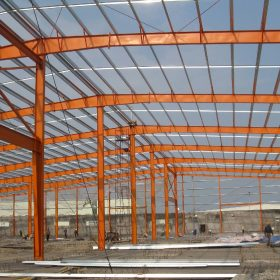
\includegraphics[width=60mm]{../../public/project-assets/yusen.jpg}};
    \fill[TTCDeepNavy,opacity=.9] (63.5,69) rectangle (122.5,88);
  \end{scope}
  \draw[TTCBorder,rounded corners=3pt] (63.5,69) rectangle (122.5,127);
  \node[anchor=west,text=white,font=\fontsize{7.5}{8.8}\selectfont\bfseries] at (68.5,81) {智慧物流仓储中心};
  \node[anchor=west,text=white!75!gray,font=\fontsize{5.8}{7}\selectfont] at (68.5,74) {超平地坪 • 升降卸货平台 • 动线优化};

  \begin{scope}
    \clip[rounded corners=3pt] (127,69) rectangle (186,127);
    \node[inner sep=0pt] at (156.5,104) {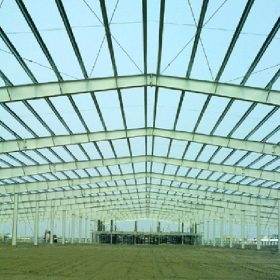
\includegraphics[width=60mm]{../../public/project-assets/sumidenso.jpg}};
    \fill[TTCDeepNavy,opacity=.9] (127,69) rectangle (186,88);
  \end{scope}
  \draw[TTCBorder,rounded corners=3pt] (127,69) rectangle (186,127);
  \node[anchor=west,text=white,font=\fontsize{7.5}{8.8}\selectfont\bfseries] at (132,81) {汽车零部件制造};
  \node[anchor=west,text=white!75!gray,font=\fontsize{5.8}{7}\selectfont] at (132,74) {日系精益品控 • 逐级放行验收};

  % 三大能力
  \node[anchor=west,text=TTCBlue,font=\fontsize{8}{9.3}\selectfont\bfseries]
    at (0,58) {贯穿所有行业的核心 EPC 总包能力};
  \foreach \xa/\xb/\title/\desc in {
    0/58/COORDINATION 全专业深化/建筑 • 结构 • 机电BIM全流程接口锁定,
    64/122/CONSTRUCTABILITY 可施工性/以现场施工工序反向指导工程深化设计,
    128/186/HANDOVER 严谨移交/凭齐备数据与实测报告逐级签署移交}
  {
    \fill[TTCLightBlue,rounded corners=3pt] (\xa,20) rectangle (\xb,50);
    \node[anchor=west,text=TTCBlue,font=\fontsize{7.2}{8.5}\selectfont\bfseries]
      at ({\xa+6},41) {\title};
    \node[anchor=north west,text width=46mm,text=TTCTextMuted,
          font=\fontsize{6.1}{7.3}\selectfont] at ({\xa+6},34) {\desc};
  }
  \fill[TTCDeepNavy,rounded corners=3pt] (0,0) rectangle (186,12);
  \node[anchor=west,text=TTCCyan,font=\fontsize{6.2}{7.4}\selectfont\bfseries] at (7,6) {SECTOR FIT};
  \node[anchor=east,text=white,font=\fontsize{7}{8.3}\selectfont\bfseries]
    at (179,6) {解决方案因工艺需求而定制 • 履约保障因专业而可靠};
\end{tikzpicture}
\end{minipage}
\newpage

% ============================================================
% TRANG 30: BỘ HỒ SƠ BÀN GIAO
% ============================================================
\noindent\mbox{}\par\vspace{-\baselineskip}
\casepagebars{竣工交付档案与可溯数据凭据}{第30页}

\begin{minipage}[t][246mm]{\textwidth}
\secbrand{全程可追溯的标准化竣工移交档案卷宗}{Evidence chain from approved material to as-built and commissioning records}

\noindent
\begin{tikzpicture}[x=1mm,y=1mm]
  \path[use as bounding box] (0,0) rectangle (186,220);
  \node[anchor=west,text=TTCBlue,font=\fontsize{15}{17}\selectfont\bfseries]
    at (0,211) {交付实体工程，同时交付完整合规的数字档案};
  \node[anchor=west,text=TTCTextMuted,font=\fontsize{7.2}{8.8}\selectfont]
    at (0,201) {每道工序只有在技术图纸、试验报告与现场影像三方一致后方可闭环归档。};

  % 5个门禁
  \fill[TTCLightBlue,rounded corners=4pt] (0,139) rectangle (186,190);
  \draw[TTCBorder,rounded corners=4pt] (0,139) rectangle (186,190);
  \draw[TTCBlue!40!white,line width=.8pt] (18,165) -- (168,165);
  \foreach \x/\n/\title in {
    18/01/材料进场,
    55.5/02/深化详图,
    93/03/工序验收,
    130.5/04/竣工图纸,
    168/05/联调联试}
  {
    \fill[white] (\x,165) circle (5mm);
    \draw[TTCBlue,line width=.8pt] (\x,165) circle (5mm);
    \node[text=TTCBlue,font=\fontsize{6}{7}\selectfont\bfseries] at (\x,165) {\n};
    \node[anchor=north,align=center,text width=29mm,text=TTCBlue,
          font=\fontsize{6.5}{7.7}\selectfont\bfseries] at (\x,155) {\title};
  }
  \fill[TTCRed] (18,165) circle (3.5mm);
  \node[text=white,font=\fontsize{5.8}{6.8}\selectfont\bfseries] at (18,165) {01};

  % 左侧卷宗
  \fill[TTCDeepNavy,rounded corners=4pt] (0,48) rectangle (70,130);
  \node[anchor=west,text=TTCCyan,font=\fontsize{7}{8.2}\selectfont\bfseries]
    at (7,121) {CLOSEOUT DOSSIER};
  \fill[white!15!gray,rounded corners=2pt] (15,61) rectangle (61,111);
  \fill[white!45!gray,rounded corners=2pt] (12,65) rectangle (58,115);
  \fill[white,rounded corners=2pt] (9,69) rectangle (55,119);
  \fill[TTCRed] (9,112) rectangle (55,119);
  \node[anchor=west,text=TTCBlue,font=\fontsize{7.4}{8.6}\selectfont\bfseries]
    at (15,103) {竣工档案卷宗};
  \draw[TTCBorder] (15,96) -- (49,96);
  \draw[TTCBorder] (15,90) -- (49,90);
  \draw[TTCBorder] (15,84) -- (42,84);
  \node[anchor=west,text=TTCTextMuted,font=\fontsize{5.8}{7}\selectfont]
    at (15,76) {CDE 统一索引 • 版本审批};
  \node[anchor=west,text=white,font=\fontsize{6.1}{7.3}\selectfont\bfseries]
    at (7,55) {单一索引库 • 模块化卷宗};

  % 右侧清单
  \fill[white,rounded corners=4pt] (76,48) rectangle (186,130);
  \draw[TTCBorder,rounded corners=4pt] (76,48) rectangle (186,130);
  \node[anchor=west,text=TTCBlue,font=\fontsize{8}{9.4}\selectfont\bfseries]
    at (83,120) {标准竣工移交档案清单架构};
  \foreach \y/\n/\title/\desc in {
    104/01/物资凭证卷宗/核准报审单 • CO/CQ 产地证 • MTC 质保书 • 试验报告,
    90/02/施工质检卷宗/ITP 检验批 • 旁站记录 • 隐蔽工程验收单,
    76/03/竣工图纸卷宗/As-built 竣工图 • 版本变动记录 • 监理业主签章,
    62/04/运维指导卷宗/O\&M 操作维保手册 • 质保承诺书 • 设备备品备件清单}
  {
    \fill[TTCLightBlue,rounded corners=2pt] (83,{\y-6}) rectangle (179,{\y+6});
    \node[anchor=west,text=TTCRed,font=\fontsize{6.2}{7.2}\selectfont\bfseries]
      at (88,\y) {\n};
    \node[anchor=west,text=TTCBlue,font=\fontsize{6.6}{7.7}\selectfont\bfseries]
      at (101,{\y+2}) {\title};
    \node[anchor=west,text=TTCTextMuted,font=\fontsize{5.6}{6.7}\selectfont]
      at (101,{\y-4}) {\desc};
  }

  % 原则
  \node[anchor=west,text=TTCBlue,font=\fontsize{8}{9.3}\selectfont\bfseries]
    at (0,37) {档案放行与移交铁律};
  \fill[TTCDeepNavy,rounded corners=3pt] (0,0) rectangle (186,29);
  \node[anchor=west,text=TTCCyan,font=\fontsize{6.2}{7.4}\selectfont\bfseries]
    at (7,20) {RELEASE CONTROL};
  \node[anchor=west,text=white,font=\fontsize{9}{10.5}\selectfont\bfseries]
    at (7,10) {严格检验 → 数据完整 → 逐级签章 → 全程可溯};
  \node[anchor=east,text=white!70!gray,font=\fontsize{6.1}{7.3}\selectfont]
    at (179,20) {唯一生效版本 • 数字化云端永久存储};
\end{tikzpicture}
\end{minipage}
\newpage

% ============================================================
% TRANG 31: NỀN TẢNG PHÁP LÝ VÀ HỆ QUẢN TRỊ
% ============================================================
\noindent\mbox{}\par\vspace{-\baselineskip}
\casepagebars{法定资质、管理体系与履约能力}{第31页}

\begin{minipage}[t][246mm]{\textwidth}
\secbrand{随时响应严格资审的法定资质与治理体系}{Corporate identity • Construction capability • ISO systems • Key-person credentials}

\noindent
\begin{tikzpicture}[x=1mm,y=1mm]
  \path[use as bounding box] (0,0) rectangle (186,220);
  \node[anchor=west,text=TTCBlue,font=\fontsize{15}{17}\selectfont\bfseries]
    at (0,211) {完备透明的企业法人身份与四重资质能力体系};
  \node[anchor=west,text=TTCTextMuted,font=\fontsize{7.2}{8.8}\selectfont]
    at (0,201) {企业法人信息、国家二级工程资质及 ISO 国际管理体系完备，满足跨国招标严苛审查。};

  % 企业基本信息
  \fill[TTCDeepNavy,rounded corners=4pt] (0,57) rectangle (67,191);
  \node[anchor=west,text=TTCCyan,font=\fontsize{7}{8.3}\selectfont\bfseries]
    at (7,182) {CORPORATE IDENTITY};
  \node[anchor=north west,text width=53mm,text=white,
        font=\fontsize{12}{14}\selectfont\bfseries]
    at (7,169) {新成功建筑科技\\股份公司};
  \draw[white!20!gray] (7,135) -- (60,135);
  \node[anchor=north west,text width=53mm,text=white!82!gray,
        font=\fontsize{6.5}{8.2}\selectfont]
    at (7,126) {\textbf{简称：} TTC JSC\\[2mm]
                 \textbf{税号：} 0107090447\\[2mm]
                 \textbf{总部：} Hà Nội, Việt Nam\\[2mm]
                 \textbf{核心业务：} 工业建筑EPC总承包、PEB钢结构制造安装、机电MEP及综合项目管理};
  \fill[TTCRed,rounded corners=2pt] (7,67) rectangle (60,82);
  \node[text=white,font=\fontsize{7}{8.2}\selectfont\bfseries] at (33.5,74.5)
    {合规 • 可溯 • 随时投标};

  % 4层能力
  \foreach \y/\n/\title/\desc in {
    166/01/国家建设活动能力证书/建设部核发工业建筑与结构施工资质，承包业务范围完全合规有效。,
    134/02/ISO 国际三体系认证/ISO 9001 质量 • ISO 14001 环境 • ISO 45001 职业安全健康国际认证齐全。,
    102/03/核心技术管理团队/项目总监、国家注册二级建造师、结构师及安全工程师配置齐全。,
    70/04/商务与资信证明材料/营业执照 • 完税证明 • 银行AAA授信证明 • 履约保函与标准投标卷宗。}
  {
    \fill[white,rounded corners=3pt] (73,{\y-13}) rectangle (186,{\y+13});
    \draw[TTCBorder,rounded corners=3pt] (73,{\y-13}) rectangle (186,{\y+13});
    \fill[TTCLightBlue,rounded corners=2pt] (79,{\y-7}) rectangle (94,{\y+7});
    \node[text=TTCRed,font=\fontsize{7}{8}\selectfont\bfseries] at (86.5,\y) {\n};
    \node[anchor=west,text=TTCBlue,font=\fontsize{7.2}{8.5}\selectfont\bfseries]
      at (101,{\y+5}) {\title};
    \node[anchor=north west,text width=76mm,text=TTCTextMuted,
          font=\fontsize{6.1}{7.4}\selectfont] at (101,{\y-1}) {\desc};
  }

  % 索引
  \node[anchor=west,text=TTCBlue,font=\fontsize{8}{9.3}\selectfont\bfseries]
    at (0,46) {资审与投标文件标准核验清单 (PRE-QUALIFICATION)};
  \foreach \xa/\xb/\label in {
    0/34/法人资格,
    38/72/施工资质,
    76/110/ISO体系,
    114/148/人员证书,
    152/186/财务资信}
  {
    \fill[TTCLightBlue,rounded corners=2pt] (\xa,20) rectangle (\xb,38);
    \node[text=TTCBlue,font=\fontsize{6.6}{7.8}\selectfont\bfseries]
      at ({(\xa+\xb)/2},29) {\label};
  }
  \fill[TTCDeepNavy,rounded corners=3pt] (0,0) rectangle (186,12);
  \node[anchor=west,text=TTCCyan,font=\fontsize{6.2}{7.4}\selectfont\bfseries] at (7,6) {DUE DILIGENCE};
  \node[anchor=east,text=white,font=\fontsize{7}{8.3}\selectfont\bfseries]
    at (179,6) {索引清晰 • 受控副本 • 快速响应跨国背调};
\end{tikzpicture}
\end{minipage}
\newpage

% ============================================================
% TRANG 32: BẢN ĐỒ HIỆN DIỆN DỰ ÁN
% ============================================================
\noindent\mbox{}\par\vspace{-\baselineskip}
\casepagebars{全国重点工业走廊业务布局图}{第32页}

\begin{minipage}[t][246mm]{\textwidth}
\secbrand{深耕越南核心经济带三大重点工业走廊}{Northern manufacturing belt • Central corridor • Southern FDI and logistics cluster}

\noindent
\begin{tikzpicture}[x=1mm,y=1mm]
  \path[use as bounding box] (0,0) rectangle (186,220);
  \node[anchor=west,text=TTCBlue,font=\fontsize{15}{17}\selectfont\bfseries]
    at (0,211) {TTC 在越南全境的工业项目分布版图};
  \node[anchor=west,text=TTCTextMuted,font=\fontsize{7.2}{8.8}\selectfont]
    at (0,201) {业务重点辐射北部高科技制造圈、中部经济走廊及南部外资与现代物流基地。};

  % 地图
  \fill[white,rounded corners=4pt] (0,24) rectangle (103,191);
  \draw[TTCBorder,rounded corners=4pt,line width=.7pt] (0,24) rectangle (103,191);
  \node[inner sep=0pt] at (51.5,107.5)
    {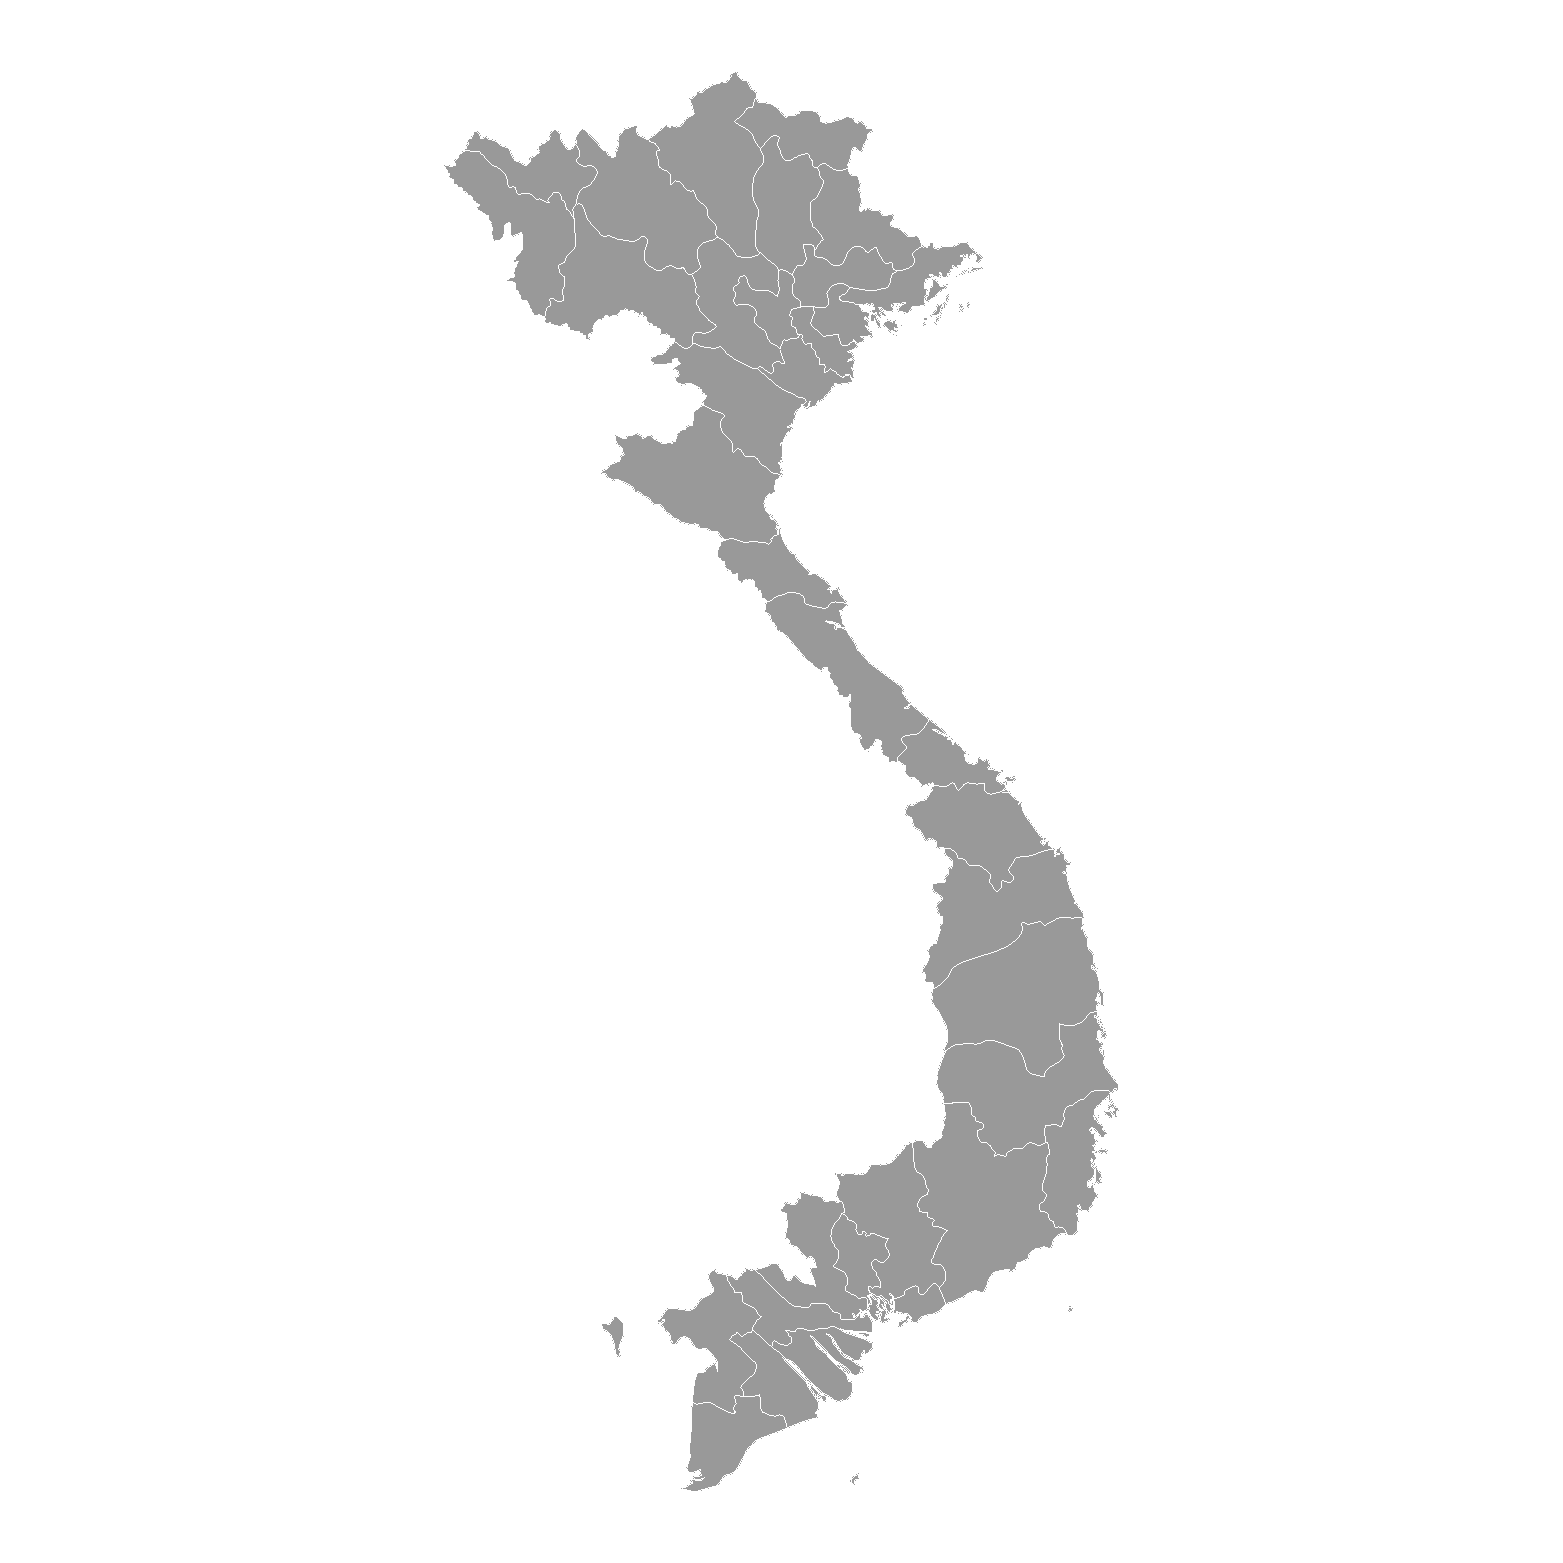
\includegraphics[height=164mm,trim=150 10 150 10,clip]{../../public/project-assets/vietnam-provinces.pdf}};

  % 圈注
  \fill[TTCRed,opacity=.16] (62,151) circle (12mm);
  \draw[TTCRed,line width=1pt] (62,151) circle (6mm);
  \fill[TTCRed] (62,151) circle (2.2mm);
  \node[anchor=west,text=TTCRed,font=\fontsize{6.5}{7.6}\selectfont\bfseries] at (70,157) {北部制造集群};
  \node[anchor=west,text=TTCTextMuted,font=\fontsize{5.5}{6.6}\selectfont] at (70,150) {河内 • 永福 • 北宁 • 北江};

  \fill[TTCBlue,opacity=.14] (62,94) circle (10mm);
  \draw[TTCBlue,line width=1pt] (62,94) circle (5mm);
  \fill[TTCBlue] (62,94) circle (2mm);
  \node[anchor=west,text=TTCBlue,font=\fontsize{6.5}{7.6}\selectfont\bfseries] at (69,100) {中部工业走廊};
  \node[anchor=west,text=TTCTextMuted,font=\fontsize{5.5}{6.6}\selectfont] at (69,93) {岘港 • 广南 • 沿海经济区};

  \fill[TTCCyan,opacity=.16] (51,51) circle (10mm);
  \draw[TTCCyan,line width=1pt] (51,51) circle (5mm);
  \fill[TTCCyan] (51,51) circle (2mm);
  \node[anchor=west,text=TTCBlue,font=\fontsize{6.5}{7.6}\selectfont\bfseries] at (59,57) {南部外资集群};
  \node[anchor=west,text=TTCTextMuted,font=\fontsize{5.5}{6.6}\selectfont] at (59,50) {平阳 • 胡志明市 • 后江};
  \node[anchor=west,text=TTCTextMuted,font=\fontsize{4.8}{5.8}\selectfont]
    at (5,29) {地图数据参考 CC0: Wikimedia Commons / Thomson Walt};

  % 右侧说明
  \fill[TTCDeepNavy,rounded corners=4pt] (109,133) rectangle (186,191);
  \node[anchor=west,text=TTCCyan,font=\fontsize{6.2}{7.4}\selectfont\bfseries]
    at (116,183) {01 • 核心根据地};
  \node[anchor=north west,text width=62mm,text=white,
        font=\fontsize{9.5}{11}\selectfont\bfseries] at (116,173) {北部重工业与电子制造带};
  \node[anchor=north west,text width=62mm,text=white!75!gray,
        font=\fontsize{6.2}{7.6}\selectfont] at (116,153) {工程密度集中于河内、永福、北宁、北江、海阳、海防与南定等各大国家级工业园区。};

  \fill[TTCLightBlue,rounded corners=4pt] (109,73) rectangle (186,127);
  \node[anchor=west,text=TTCRed,font=\fontsize{6.2}{7.4}\selectfont\bfseries]
    at (116,119) {02 • 快速机动调配};
  \node[anchor=north west,text width=62mm,text=TTCBlue,
        font=\fontsize{8.5}{10}\selectfont\bfseries] at (116,109) {跨区域项目团队保障};
  \node[anchor=north west,text width=62mm,text=TTCTextMuted,
        font=\fontsize{6.2}{7.6}\selectfont] at (116,92) {依据项目群设常驻工程总监、QA/QC与HSE工程师，重型机械装备按工序精准调度。};

  \fill[white,rounded corners=4pt] (109,24) rectangle (186,67);
  \draw[TTCBorder,rounded corners=4pt] (109,24) rectangle (186,67);
  \node[anchor=west,text=TTCBlue,font=\fontsize{6.2}{7.4}\selectfont\bfseries]
    at (116,59) {03 • 重点拓展方向};
  \node[anchor=north west,text width=62mm,text=TTCTextDark,
        font=\fontsize{6.3}{7.7}\selectfont] at (116,49) {有选择性地扩大中部及南部高端工业市场，重点服务跨国大型EPC外资厂房及冷链智慧物流基地。};

  \fill[TTCDeepNavy,rounded corners=3pt] (109,0) rectangle (186,16);
  \node[anchor=west,text=TTCCyan,font=\fontsize{6.1}{7.2}\selectfont\bfseries]
    at (116,8) {PROJECT FOOTPRINT};
  \node[anchor=east,text=white,font=\fontsize{6.5}{7.7}\selectfont\bfseries]
    at (179,8) {覆盖全国 20+ 工业重镇省市};
\end{tikzpicture}
\end{minipage}
\newpage

% ============================================================
% TRANG 33: LỘ TRÌNH 2026--2030
% ============================================================
\noindent\mbox{}\par\vspace{-\baselineskip}
\casepagebars{2026--2030 战略发展规划与稳健成长路线图}{第33页}

\begin{minipage}[t][246mm]{\textwidth}
\secbrand{精选优质工程 • 稳健健康的战略发展路线图}{Controlled growth • Repeat clients • High-tech capability • Positive cash discipline}

\noindent
\begin{tikzpicture}[x=1mm,y=1mm]
  \path[use as bounding box] (0,0) rectangle (186,220);
  \node[anchor=west,text=TTCBlue,font=\fontsize{15}{17}\selectfont\bfseries]
    at (0,211) {以健全稳健的治理能力驱动业务规模高质量增长};
  \node[anchor=west,text=TTCTextMuted,font=\fontsize{7.2}{8.8}\selectfont]
    at (0,201) {坚持审慎务实的经营方针，将现金流健康度与高品质交付置于盲目扩张之前。};

  % 3个发展阶段
  \foreach \xa/\xb/\year/\value/\focus/\desc in {
    0/58/2026年/300--400 亿越盾/夯实治理底座/全面推行CDE云端数字化 • 严控成本基线 • 深耕北部核心根据地,
    64/122/2027--2028年/依能力稳步提质/精选高附加值/扩大半导体洁净厂房与高科技工程占比 • 提升老客户复签率,
    128/186/2029--2030年/依现金流规模化/可持续领跑/稳健拓展全境及区域市场 • 成为越南顶尖工业建筑总包商}
  {
    \fill[white,rounded corners=4pt] (\xa,68) rectangle (\xb,190);
    \draw[TTCBorder,rounded corners=4pt,line width=.7pt] (\xa,68) rectangle (\xb,190);
    \fill[TTCDeepNavy,rounded corners=4pt] (\xa,165) rectangle (\xb,190);
    \node[anchor=west,text=TTCCyan,font=\fontsize{7}{8.3}\selectfont\bfseries]
      at ({\xa+6},181) {\year};
    \node[anchor=west,text=white,font=\fontsize{13}{15}\selectfont\bfseries]
      at ({\xa+6},171) {\value};
    \fill[TTCRed] ({\xa+6},153) rectangle ({\xa+22},155);
    \node[anchor=west,text=TTCBlue,font=\fontsize{7.6}{9}\selectfont\bfseries]
      at ({\xa+6},143) {\focus};
    \node[anchor=north west,text width=46mm,text=TTCTextMuted,
          font=\fontsize{6.3}{7.7}\selectfont] at ({\xa+6},133) {\desc};
    \node[anchor=south west,text width=46mm,text=TTCTextDark,
          font=\fontsize{6.1}{7.5}\selectfont] at ({\xa+6},78)
      {\textbf{升级考核指标：} 净利润率、正向现金流与核心技术骨干储备完全达标。};
  }

  % 亮点
  \foreach \y/\label in {116/CDE 协同平台,104/严控成本基线,92/深耕北部根据地}{
    \fill[TTCRed] (6,\y) circle (1.2mm);
    \node[anchor=west,text=TTCTextDark,font=\fontsize{6.2}{7.4}\selectfont] at (11,\y) {\label};
  }
  \foreach \y/\label in {116/洁净室与高科技,104/老客户高复购率,92/多项目协同管控}{
    \fill[TTCRed] (70,\y) circle (1.2mm);
    \node[anchor=west,text=TTCTextDark,font=\fontsize{6.2}{7.4}\selectfont] at (75,\y) {\label};
  }
  \foreach \y/\label in {116/精选优质 EPC,104/审慎跨区布局,92/绿色低碳供应链}{
    \fill[TTCRed] (134,\y) circle (1.2mm);
    \node[anchor=west,text=TTCTextDark,font=\fontsize{6.2}{7.4}\selectfont] at (139,\y) {\label};
  }

  % 4道筛选机制
  \node[anchor=west,text=TTCBlue,font=\fontsize{8}{9.3}\selectfont\bfseries]
    at (0,57) {项目承接四大内控筛选准入原则};
  \foreach \xa/\xb/\n/\label in {
    0/43.5/01/正向现金流保障,
    47.5/91/02/核心团队就绪,
    95/138.5/03/合同法律风险锁定,
    142.5/186/04/100\%确定性交付}
  {
    \fill[TTCLightBlue,rounded corners=3pt] (\xa,25) rectangle (\xb,49);
    \node[anchor=west,text=TTCRed,font=\fontsize{6}{7}\selectfont\bfseries]
      at ({\xa+5},40) {\n};
    \node[anchor=west,text=TTCBlue,font=\fontsize{6.2}{7.4}\selectfont\bfseries]
      at ({\xa+5},32) {\label};
  }
  \node[anchor=west,text=TTCTextMuted,font=\fontsize{5.4}{6.5}\selectfont\itshape]
    at (0,14) {注：相关数据为公司内部战略规划与管理目标，非对外财务盈利预测。};
  \fill[TTCDeepNavy,rounded corners=3pt] (0,0) rectangle (186,10);
  \node[anchor=west,text=TTCCyan,font=\fontsize{6}{7.2}\selectfont\bfseries] at (7,5) {CONTROLLED GROWTH};
  \node[anchor=east,text=white,font=\fontsize{6.8}{8}\selectfont\bfseries]
    at (179,5) {营收质量与交付口碑重于单纯规模扩张};
\end{tikzpicture}
\end{minipage}
\newpage

% ============================================================
% TRANG 34: BẢO HÀNH VÀ HẬU MÃI
% ============================================================
\noindent\mbox{}\par\vspace{-\baselineskip}
\casepagebars{24个月质保承诺与终身运维支持}{第34页}

\begin{minipage}[t][246mm]{\textwidth}
\secbrand{单一窗口全生命周期售后维保支持}{24/7 intake • Contract-based response • Field verification • Closed-loop records}

\noindent
\begin{tikzpicture}[x=1mm,y=1mm]
  \path[use as bounding box] (0,0) rectangle (186,220);
  \node[anchor=west,text=TTCBlue,font=\fontsize{15}{17}\selectfont\bfseries]
    at (0,211) {工程交付并非终点 — 而是长期伙伴合作的新起点};
  \node[anchor=west,text=TTCTextMuted,font=\fontsize{7.2}{8.8}\selectfont]
    at (0,201) {竣工后所有维保需求均由专职售后工程团队统一受理、精准处置与闭环归档。};

  % 24个月承诺
  \fill[TTCDeepNavy,rounded corners=4pt] (0,141) rectangle (54,190);
  \node[anchor=west,text=TTCCyan,font=\fontsize{6.4}{7.6}\selectfont\bfseries]
    at (7,181) {全方位标准质保};
  \node[anchor=west,text=white,font=\fontsize{23}{25}\selectfont\bfseries]
    at (7,162) {24 个月};
  \node[anchor=west,text=white!72!gray,font=\fontsize{5.9}{7.1}\selectfont]
    at (7,149) {主体结构享终身维保支持};

  \fill[TTCLightBlue,rounded corners=4pt] (60,141) rectangle (186,190);
  \node[anchor=west,text=TTCBlue,font=\fontsize{8}{9.3}\selectfont\bfseries]
    at (67,181) {单一维保责任窗口 — 闭环追踪处理记录};
  \node[anchor=north west,text width=104mm,text=TTCTextDark,
        font=\fontsize{6.7}{8.2}\selectfont] at (67,171)
    {设有 24/7 应急服务热线与技术专员。根据故障等级，维保团队在合同约定时间内迅速赶赴现场并提出有效解决方案。};
  \node[anchor=west,text=TTCRed,font=\fontsize{6.4}{7.6}\selectfont\bfseries]
    at (67,149) {绝无模糊推诿 • 未经业主签字确认绝不关闭维保工单};

  % 流程
  \node[anchor=west,text=TTCBlue,font=\fontsize{8}{9.3}\selectfont\bfseries]
    at (0,130) {标准化售后维保闭环服务流程};
  \foreach \xa/\xb/\n/\title/\desc in {
    0/42/01/工单受理/登记现场情况 • 影响程度与照片,
    48/90/02/定级分派/界定保修范围与紧急响应等级,
    96/138/03/现场处置/工程技术人员现场排查与维修施工,
    144/186/04/签字闭环/业主验收合格 • 归入工程运维档案}
  {
    \fill[white,rounded corners=3pt] (\xa,78) rectangle (\xb,121);
    \draw[TTCBorder,rounded corners=3pt] (\xa,78) rectangle (\xb,121);
    \fill[TTCRed,rounded corners=1pt] ({\xa+5},109) rectangle ({\xa+16},118);
    \node[text=white,font=\fontsize{6}{7}\selectfont\bfseries] at ({\xa+10.5},113.5) {\n};
    \node[anchor=west,text=TTCBlue,font=\fontsize{7}{8.2}\selectfont\bfseries]
      at ({\xa+5},101) {\title};
    \node[anchor=north west,text width=31mm,text=TTCTextMuted,
          font=\fontsize{5.9}{7.2}\selectfont] at ({\xa+5},94) {\desc};
  }
  \foreach \xa/\xb in {42/48,90/96,138/144}{
    \draw[-{Latex[length=2mm]},TTCBlue!65!white,line width=.8pt]
      ({\xa+1},99) -- ({\xb-1},99);
  }

  % 分项
  \node[anchor=west,text=TTCBlue,font=\fontsize{8}{9.3}\selectfont\bfseries]
    at (0,67) {保修范围严格依照合同及竣工验收纪要约定};
  \foreach \xa/\xb/\title/\desc in {
    0/58/结构工程/刚架 • 节点高强螺栓 • 基础与防腐涂层,
    64/122/围护系统/屋面防水 • 泛水板 • 天沟雨水系统 • 夹芯板,
    128/186/机电与消防/电气系统 • 暖通空调 • 消防管网与泵房}
  {
    \fill[TTCLightBlue,rounded corners=3pt] (\xa,25) rectangle (\xb,58);
    \node[anchor=west,text=TTCBlue,font=\fontsize{7.2}{8.5}\selectfont\bfseries]
      at ({\xa+6},48) {\title};
    \node[anchor=north west,text width=46mm,text=TTCTextMuted,
          font=\fontsize{6}{7.3}\selectfont] at ({\xa+6},40) {\desc};
  }
  \fill[TTCDeepNavy,rounded corners=3pt] (0,0) rectangle (186,16);
  \node[anchor=west,text=TTCCyan,font=\fontsize{6.1}{7.3}\selectfont\bfseries] at (7,8) {SERVICE DESK 24/7};
  \node[anchor=east,text=white,font=\fontsize{6.8}{8}\selectfont\bfseries]
    at (179,8) {快速接单 → 精准处置 → 业主确认 → 留痕归档};
\end{tikzpicture}
\end{minipage}
\newpage

% ============================================================
% TRANG 35: HỆ SINH THÁI ĐỐI TÁC — LOGO WALL
% ============================================================
\noindent\mbox{}\par\vspace{-\baselineskip}
\casepagebars{战略合作伙伴与金融机构生态圈}{第35页}

\begin{minipage}[t][246mm]{\textwidth}
\secbrand{战略生态合作伙伴与授信金融机构}{Selected corporate and financial partners in the TTC network}

\noindent
\begin{tikzpicture}[x=1mm,y=1mm]
  \path[use as bounding box] (0,0) rectangle (186,220);

  \node[anchor=west,text=TTCBlue,font=\fontsize{15}{17}\selectfont\bfseries]
    at (0,211) {汇聚产业链优质资源 • 赋能工程卓越履约};
  \node[anchor=west,text width=178mm,text=TTCTextMuted,
        font=\fontsize{7.2}{8.8}\selectfont]
    at (0,199) {TTC 与各领域龙头企业及各大商业银行建立稳固的战略合作伙伴关系，资金与供应链实力雄厚。};

  % 企业合作伙伴
  \fill[TTCLightBlue,rounded corners=3pt] (0,177) rectangle (186,191);
  \node[anchor=west,text=TTCCyan,font=\fontsize{6.2}{7.4}\selectfont\bfseries]
    at (7,184) {CORPORATE ECOSYSTEM};
  \node[anchor=east,text=TTCBlue,font=\fontsize{7.2}{8.6}\selectfont\bfseries]
    at (179,184) {战略企业生态圈};

  \newcommand{\corporatelogoclosing}[3]{%
    \fill[white,rounded corners=3pt] (#1,#2) rectangle ({#1+43.5},{#2+31});
    \draw[TTCBorder,rounded corners=3pt,line width=.6pt]
      (#1,#2) rectangle ({#1+43.5},{#2+31});
    \fill[TTCRed] ({#1+4},{#2+25.5}) rectangle ({#1+12},{#2+27});
    \node[inner sep=0pt] at ({#1+21.75},{#2+15})
      {\includegraphics[width=29mm,height=23mm,keepaspectratio]{#3}};
  }

  \corporatelogoclosing{0}{139}{../../public/logo/Food-logo.png}
  \corporatelogoclosing{47.5}{139}{../../public/logo/aidc_logo.png}
  \corporatelogoclosing{95}{139}{../../public/logo/alo-logo.png}
  \corporatelogoclosing{142.5}{139}{../../public/logo/company-minhphu.png}
  \corporatelogoclosing{0}{103}{../../public/logo/dieuphuong-logo.png}
  \corporatelogoclosing{47.5}{103}{../../public/logo/par5.png}
  \corporatelogoclosing{95}{103}{../../public/logo/y2y.png}
  \corporatelogoclosing{142.5}{103}{../../public/logo/company-sinchi.png}

  % 银行
  \fill[TTCLightBlue,rounded corners=3pt] (0,82) rectangle (186,96);
  \node[anchor=west,text=TTCCyan,font=\fontsize{6.2}{7.4}\selectfont\bfseries]
    at (7,89) {FINANCIAL PARTNERS};
  \node[anchor=east,text=TTCBlue,font=\fontsize{7.2}{8.6}\selectfont\bfseries]
    at (179,89) {银行授信金融合作伙伴};

  \newcommand{\banklogoclosing}[2]{%
    \fill[white,rounded corners=3pt] (#1,39) rectangle ({#1+28.5},75);
    \draw[TTCBorder,rounded corners=3pt,line width=.55pt]
      (#1,39) rectangle ({#1+28.5},75);
    \node[inner sep=0pt] at ({#1+14.25},57)
      {\includegraphics[width=23mm,height=17mm,keepaspectratio]{#2}};
  }
  \banklogoclosing{0}{../../public/logo/bank-acb.pdf}
  \banklogoclosing{31.5}{../../public/logo/bank-tpbank.pdf}
  \banklogoclosing{63}{../../public/logo/bank-vietcombank.pdf}
  \banklogoclosing{94.5}{../../public/logo/bank-bidv.pdf}
  \banklogoclosing{126}{../../public/logo/bank-vietinbank.png}
  \banklogoclosing{157.5}{../../public/logo/bank-mb.png}

  \fill[TTCDeepNavy,rounded corners=3pt] (0,0) rectangle (186,24);
  \fill[TTCRed,rounded corners=1pt] (7,7) rectangle (9,17);
  \node[anchor=west,text=white,font=\fontsize{8.4}{10}\selectfont\bfseries]
    at (15,15) {深度协同 • 创造更大商业价值};
  \node[anchor=west,text=white!70!gray,font=\fontsize{6.1}{7.4}\selectfont]
    at (15,7) {融合专业优势、供应链资源与充沛金融资本，为业主工程保驾护航。};
  \node[anchor=east,text=TTCCyan,font=\fontsize{6.4}{7.6}\selectfont\bfseries]
    at (179,12) {PARTNERSHIP BUILT ON TRUST};
\end{tikzpicture}
\end{minipage}
\newpage

% ============================================================
% TRANG 36: BÌA SAU — NHẬN DIỆN THƯƠNG HIỆU
% ============================================================
\thispagestyle{empty}
\begin{tikzpicture}[remember picture,overlay]
  \fill[TTCDeepNavy] (current page.south west) rectangle (current page.north east);
  \fill[TTCRed] (current page.north west) rectangle ([yshift=-3mm]current page.north east);
  \fill[TTCRed] (current page.south west) rectangle ([yshift=3mm]current page.south east);

  \begin{scope}[opacity=.075]
    \draw[white,line width=.8pt]
      ([xshift=16mm,yshift=122mm]current page.south west)
      -- ([xshift=16mm,yshift=146mm]current page.south west)
      -- ([xshift=52mm,yshift=168mm]current page.south west)
      -- ([xshift=88mm,yshift=146mm]current page.south west)
      -- ([xshift=124mm,yshift=178mm]current page.south west)
      -- ([xshift=158mm,yshift=146mm]current page.south west)
      -- ([xshift=194mm,yshift=166mm]current page.south west)
      -- ([xshift=194mm,yshift=122mm]current page.south west);
    \foreach \x in {28,40,64,76,100,112,136,148,172,184}{
      \draw[white,line width=.4pt]
        ([xshift=\x mm,yshift=122mm]current page.south west)
        -- ([xshift=\x mm,yshift=147mm]current page.south west);
    }
  \end{scope}
  \node[text=white,opacity=.025,font=\fontsize{92}{96}\selectfont\bfseries]
    at ([yshift=8mm]current page.center) {TTC};

  % 顶部 Logo
  \node[anchor=north west,fill=white,rounded corners=4pt,
        inner xsep=7mm,inner ysep=4mm]
    at ([xshift=17mm,yshift=-20mm]current page.north west)
    {
\includegraphics[width=57mm]{../../public/logo-ttc-removebg-DNXrVdJp.png}};
  \node[anchor=north east,text=white!75!gray,font=\fontsize{6.5}{7.8}\selectfont\bfseries]
    at ([xshift=-17mm,yshift=-24mm]current page.north east) {COMPANY PROFILE • 2026};

  \node[anchor=north west,text=TTCCyan,font=\fontsize{7.5}{9}\selectfont\bfseries]
    at ([xshift=18mm,yshift=-78mm]current page.north west) {INDUSTRIAL DESIGN • BUILD • DELIVERY};
  \node[anchor=north west,text width=174mm,text=white,
        font=\fontsize{28}{31}\selectfont\bfseries]
    at ([xshift=18mm,yshift=-94mm]current page.north west)
    {携手共建 • 赋能卓越};
  \fill[TTCRed] ([xshift=18mm,yshift=-164mm]current page.north west)
    rectangle ([xshift=60mm,yshift=-167mm]current page.north west);
  \node[anchor=north west,text width=170mm,text=white!78!gray,
        font=\fontsize{8.2}{10.6}\selectfont]
    at ([xshift=18mm,yshift=-178mm]current page.north west)
    {新成功建筑科技 (TTC) 愿从投资策划、工程设计、施工总包到终身运维，全程为您在越南的工业投资保驾护航。};

  % 底部联系卡片
  \fill[white,rounded corners=5pt]
    ([xshift=17mm,yshift=25mm]current page.south west)
    rectangle ([xshift=-17mm,yshift=104mm]current page.south east);
  \node[anchor=north west,text=TTCBlue,font=\fontsize{9.2}{11}\selectfont\bfseries]
    at ([xshift=26mm,yshift=94mm]current page.south west)
    {新成功建筑科技股份公司};
  \node[anchor=north west,text=TTCTextMuted,font=\fontsize{5.8}{7}\selectfont\bfseries]
    at ([xshift=26mm,yshift=83mm]current page.south west)
    {TAN THANH CONG TECHNOLOGY CONSTRUCTION JOINT STOCK COMPANY};
  \draw[TTCBorder,line width=.6pt]
    ([xshift=26mm,yshift=75mm]current page.south west)
    -- ([xshift=-26mm,yshift=75mm]current page.south east);

  \node[anchor=north west,text width=148mm,text=TTCTextDark,
        font=\fontsize{7}{9.2}\selectfont]
    at ([xshift=26mm,yshift=69mm]current page.south west)
    {\textcolor{TTCRed}{\faMapMarker*}\quad
     \textbf{注册地址：} Số 39, ngõ 292 Kim Giang, Đại Kim, Hà Nội\\[2.3mm]
     \textcolor{TTCRed}{\faBuilding}\quad
     \textbf{商务办公：} Số 19N7B, KĐT Trung Hòa Nhân Chính, Hà Nội\\[2.3mm]
     \textcolor{TTCRed}{\faPhone*}\quad +84 976 447 766
     \hspace{12mm}\textcolor{TTCRed}{\faEnvelope}\quad info@tanthanhcongjsc.com
     \hspace{12mm}\textcolor{TTCRed}{\faGlobe}\quad tanthanhcongjsc.com};

  \node[anchor=south west,text=white!65!gray,font=\fontsize{5.6}{6.8}\selectfont]
    at ([xshift=17mm,yshift=8mm]current page.south west)
    {\textcopyright\ 2026 新成功建筑科技股份公司 (TTC JSC)};
  \node[anchor=south east,text=TTCCyan,font=\fontsize{6.2}{7.4}\selectfont\bfseries]
    at ([xshift=-17mm,yshift=8mm]current page.south east)
    {TANTHANHCONGJSC.COM};
\end{tikzpicture}


\end{document}
